%\documentclass[12pt]{report}
%\usepackage[utf8]{inputenc}
%\usepackage{graphicx}
%\graphicspath{{images/}}
%\usepackage{pdfpages}
%\usepackage{booktabs}
%\usepackage[british]{babel}
%\usepackage{csquotes}
%\usepackage[backend=biber,style=apa,sorting=nyt,natbib=true]{biblatex}
%\DeclareLanguageMapping{british}{british-apa}
%\addbibresource{references.bib}
%\usepackage{cleveref}
%\newcommand{\crefrangeconjunction}{ to~}
%\usepackage{enumitem}
%\setlist[description]{leftmargin=\parindent,labelindent=\parindent}
%\newcommand{\myparagraph}[1]{\paragraph{#1}\mbox{}\\}
%\usepackage{geometry}
%\usepackage{pdflscape}
%\usepackage{amsmath}

%\title{
%{National Tournament Survey Study}\\
%{Qianan, Hebei Province, July 16-17 2016}
%}
%\author{Jacob Taylor}



%\begin{document}

%\maketitle{}


%\tableofcontents
%\clearpage


\chapter{\label{tournamentSurvey}National Tournament Survey Study}


\section{Abstract}
The following survey study was designed to analyse the relationship between joint-action and social bonding among professional Chinese rugby players in a naturalistic real-world setting. The study took place in the context of a two-day National Rugby Sevens Tournament in Qianan, Hebei Province, China July 16-17 2016 (the Tournament).  Self-report survey and Tournament performance data were collected from 174 adult rugby playing athletes ($male = 93, M = 21.67, SD = 3.67, range = 17-32$). Data were analysed according to predictions derived from existing theory of joint-action and social bonding, as well as ethnographic observations. Specifically, the study aimed to analyse the hypothesis that feelings of ``team click'' mediate a relationship between perceptions of joint-action success and social bonding.

\section{Introduction}

Intro:


Lit Review:


Closing:




%In this study, professional rugby players were surveyed before, during, and after a high-intensity, high-stakes National professional rugby tournament.

\subsection{Predictions}
This study tested the following predictions regarding the relationship between joint-action and social bonding.  On average, and controlling for perceptions of individual performance and objective measures of success individual and team success in the Tournament:
\begin{indent}
\begin{description}
  \item [Prediction 1.a] Athletes who perceive greater success in joint-action will experience higher levels of felt  ``team click.''
  \item [Prediction 1.b] Athletes who experience more positive violation of expectation around team performance will experience higher levels of team click.
  \item [Prediction 1.c] Athletes who perceive greater success in joint-action as a more positive violation of prior expectations will experience higher levels of team click”.
  OR: Athletes with a stronger association between perceived success in JA and positive violation of prior expectations will experience higher levels of team click.  \\

  \item [Prediction 2.a] Athletes who experience higher levels of team click will report higher levels of social bonding.
  \bigskip
  \item [Prediction 3.a] Higher perceived success in joint-action will predict higher levels of social bonding.
 \item [Prediction 3.b] Greater positive violation of expectations around team performance will predict higher levels of social bonding.
  \item [Prediction 4.a] Team click will mediate the positive relationship between joint-action success and social bonding.
  \item [Prediction 4.b] Team click will mediate the positive relationship between positive violation of performance expectations and social bonding.
\end{description}
\end{indent}







\section{Method}

\subsection{Participants}
174 Chinese professional adult rugby players from 8 men’s provincial teams and 7 women’s provincial teams were surveyed  (mean athletes per team = 11.6 ($SD =1.06$), $male = 93$, $M(age) = 21.67$ ($SD = 3.67$, $range = 16 - 32$))---once before (2-4 days before, $n = 120$), twice during (once each day of the two day tournament, following the 2nd or 3rd game of each day, $n = 164$), and once after the Tournament ($n = 118$).  The University of Oxford’s Central University Research Ethics Committee approved this study (SAME/CUREC1A/15-059).


\subsection{Materials}

\subsubsection{The Tournament}
``The Chinese National Rugby Sevens Championship'' was held 16-17th July 2016 in Qianan, Hebei Province, China. The Tournament was the most important of the four national-level tournaments held in 2016 because results in the Tournament decided the title of overall men's and women’s national champion. The rugby players surveyed in the Tournament represent the top level of current professional rugby playing athletes in China.

A rugby sevens tournament generally requires two full days to complete, and most teams play an average of 5 or 6 games in total. Within each tournament, participating teams are first divided into smaller pools, and spend the first day of the tournament playing a 14-minute game against every team in their pool. On the second day of the tournament, teams are re-grouped according to Day 1 results, and play in a three-round knock out phase to decide overall placings (usually quarter-, semi- and grand-final structure). On day 2, the top 8 teams of the tournament compete for overall championship in a quarter-semi-grand final format, and any remaining teams compete for the remaining placings below these 8 teams. The playing time for the grand-final is extended to 20 minutes (10 minutes per half, as opposed to the usual 7 minutes).

In this particular Tournament, seven women's teams and eight men's teams participated.  The men’s competition was split into two pools of four teams each, and the women’s competition was split into one pool of four and one pool of three teams (see Table~\ref{tab:poolStructure}). \\


\begin{table}[htpb]\caption{Tournament Pool Structure}
  \begin{center}
    \begin{small}
        \begin{tabular}{| c | c || c | c |}
          \hline
          \bf Women's Pool A & \bf Women's Pool B &  \bf Men's Pool A & \bf  Men's Pool B \\
          \hline
          Jiangsu & Anhui & Shandong & Tianjin \\
          Shandong & Shanghai & Beijing & PLA\superscript{*} \\
          Tianjin & Beijing & Hebei & Anhui \\
             & Fujian & Shanghai & Fujian \\
             \hline
        \end{tabular}
          \end{small}
        \end{center}

        \begin{footnotesize}
          $^*$People's Liberation Army
        \end{footnotesize}

  \label{tab:poolStructure}
    \end{table}



\subsection{Surveys}
Surveys were generated using Qualtrics software (Qualtrics version 9, Provo, UT). Surveys were translated into Chinese and then back translated by two independent native Chinese speaking translators from Beijing Sports University.  Pre- and post-Tournament surveys were administered online using a social networking software called WeChat. WeChat is an online messaging and social networking platform that has become a near-universal means of electronic communication in Mainland China (an English language/Western equivalent would be something of a cross between Facebook and WhatsApp Messenger). The surveys administered before and after the Tournament were completed by athletes within the WeChat application, using their personal mobile phone devices and Internet access. Due to the constraints of the Tournament setting, in particular athletes’ lack of access to mobile phones and Internet immediately following games, meant that hard copy (paper) surveys rather than electronic surveys were administered mid-Tournament.


\subsection{Survey Items}
Surveys were designed according to theoretically and ethnographically derived predictions about athlete experience of high-intensity competition.  In the pre-Tournament, mid-Tournament, and post-Tournament surveys, athletes were asked to report their subjective experience of individual and team performance, overall feeling about the quality of team coordination or \textbf{``team click''}, and feelings of social bonding.  In addition, athletes were asked about feelings of exertion, fatigue, injury, as well as objective and subjective measures of technical competence, perceptions of team discipline, and individual personality type.

%% Summary table of key variables, ned to adapt from Ch6
%<<surveyMeasureSummaryTable, eval=T, echo=F>>=
%  #create all columns:
%  Items <- c("Performance(Ind)", "Performance(Group)", "Performance(Team)",
%             "TeamClick(Group)", "TeamClick(Team)", "SocialBonding(Group)", %"SocialBonding(Team)", "Arousal", "Exertion")
%  Baseline <- c("*","","*","","*","","*","","")
%  Pre <- c("*","*","","*","","*","","*","")
%  Post <- c("*","*","","*","*","*","*","*","*")

%  surveyMeasureSummary <- data.frame(Items, Baseline, Pre, Post, stringsAsFactors = FALSE)

%  summaryTable <- xtable(surveyMeasureSummary,
%                                caption = "Survey items measured at each time point"
%                                label = "tab:surveyItemsByTime")
%  align(summaryTable) <- "llccc"
%  print(summaryTable, file="surveyItemsByTime.tex")
%@

  \subsubsection{Pre-Tournament Survey Items}

    \myparagraph{Overall and Component Performance}

In the pre-Tournament survey, Athletes were asked to reflect on the \textit{overall} quality of performance, as well the quality of specific \textit{components} of individual and team performance.  Questions concerning overall team and individual performance were framed in terms of the month of training and competition prior to date of the survey, for example: ``Overall, how well do you feel your team has been performing in training and competition over the past month?''
Athletes responded to each item by moving a toggle left or right from its default centre position on a continuous 100-point scale (0 = ``Extremely poor,'' 100 = ``Extremely well'').

Athletes were also asked to report their impression of the quality of \textit{components} of individual and team performance commonly scrutinised throughout the course of the researcher's ethnographic observations and in rugby union more generally.  Individual components of performance included 1) passing technique, 2) support play in attack, 3) one-on-one defence, 4) effectiveness in contact, and 5) decision making in game play.  Components of team performance included 1) coordination of the defensive line, 2) coordination of the attacking line, 3) support play, and 4) on-field communication.  In the pre-Tournament survey, athletes were asked about their impression of team or individual performance in the past month, for example: ``how do you feel about your team's coordination of the defensive line over the past month?''  In the post-Tournament survey athletes were asked about their impressions of the same components of performance as they experienced them in the Tournament itself, e.g. ``How do you feel about your passing technique during the Tournament?'' Athletes responded to each item by moving a toggle left or right from its default centre position on a continuous 100-point scale: 0 - ``Extremely poor'', 100 - ``Extremely good.''  Athletes were also asked to report the extent to which 1) the quality of recent individual performances influences their mood, 2) recent performance influences their confidence for future performance.


  \myparagraph{Team Click}
Athletes were asked about their feelings about their team's overall on-field coordination in the past month, also known as ``team click''. Survey items pertaining to team click were generated by utilising phrasing commonly encountered by the researcher during ethnographic observations of the Beijing provincial team and other provincial teams.  Team click items included the feeling of ``unspoken understanding'' (\textit{moqi}) between team mates, the ``general atmosphere'' of the team, the reliability of athletes' teammates to perform their roles on the field, the reliability of individual athletes to perform their on-field roles for teammates, and the extent to which athletes felt that their individual abilities were extended by their team mates.  Athletes responded to each item by moving a toggle left or right from its default centre position on a continuous 100-point scale. In addition to these items, a novel visual item with five responses, ranging from less to more coordinated arrangements of dots, was used to understand athletes' feelings of team click (see Appendix ~\ref{app5:tournamentSurvey} Section ~\ref{app5:clickPre} for a detailed explanation of all pre-Tournament survey items relevant to team click).

  \myparagraph{Social Bonding}
A number of survey items were included in the pre-Tournament survey in order to access athlete feelings social bonding to their team.  Athletes were asked to report the extent to which they felt 1) emotional support from teammates and 2) a sense of shared goal with their team mates (100-point scale, 0 - ``Extremely weak'', 100 - ``Extremely strong'').  Athletes completed two validated multi-item scales designed to measure 1) an individual's personal identification with the stereotypical features of the in-group \citep[Group Identification Verbal Scale, see][]{Mael1992} and 2) an individual's fusion or ``feeling of oneness with the group'' \citep[Identity Fusion Verbal Scale, see][]{Swann2009}. A visual scale designed to measure construct of Identity Fusion to the target in-group \citep{Swann2009} was included for three targets: the athletes' team, family, and nationality (``China'').  Finally,  Athletes ranked their level of Identity Fusion to team, family, and country \citep[replicating][]{Whitehouse2014}.  See Appendix ~\ref{app5:tournamentSurvey} Section ~\ref{app5:bondingPre} for a detailed explanation of all pre-Tournament items relevant to social bonding.

  \myparagraph{Technical Competence}
In order to measure individual competence in the technical demands of rugby, athletes were asked to report their perceptions of individual technical competence relative to 1) other teammates, 2 other current professional Chinese rugby players, and  3) Professional rugby players form other countries.  In addition, athletes were asked to report rugby-related attributes that would provide a more objective indicator of technical competence. These measures included: 1) rugby training age (number of years of experience training for rugby, to the nearest number of years), 2) the number of years spent training with the provincial teams (to the nearest year) and 3) whether the athlete is a usual member of the provincial program's starting team or the reserves.  See Appendix ~\ref{app5:tournamentSurvey} Section ~\ref{app5:technicalCompetence} for a detailed explanation of all items relating to technical competence.

  \myparagraph{Personality}
Due to the hypothesised links between personality type and dispositional tendencies towards interpersonal coordination strategies \citep[see for example][]{Marsh2009}, a ten-item personality measure was included in the pre-Tournament survey (Ten Item Personality Index - TIPI)\citep{Gosling2003}. See Appendix ~\ref{app5:tournamentSurvey} Section ~\ref{app5:TIPI} for a detailed explanation.

\myparagraph{Additional Items}

For a detailed description of additional items included in the pre-Tournament survey, see Appendix ~\ref{app5:tournamentSurvey} Section ~\ref{app5:additionalItems}
Team Discipline
Injury Status
IDVars: name age team








\subsubsection{Mid-Tournament Survey Items}


\begin{description}
\item [Individual Performance Expectations]``Overall, how do you feel about your individual performance in this game?''
\item [Team Performance Expectations] ``Overall, how do you feel about your team's performance in this game?''
\end{description}
Both items used a zero-centred continuous scale, -50 = ``much worse than expected'', 0 =  ``As expected'', 50 =  ``much better than expected''.








\subsubsection{Post-Tournament Survey Items}

The post-Tournament survey repeated the mid-Tournament items, asking:
\begin{description}
\item [Individual Performance Expectations] ``Overall, how do you feel about your individual performance during the tournament?''
\item [Team Performance Expectations]``Overall, how do you feel about your team's performance during the tournament?''
\end{description}


While these four items did not provide a measure of performance in relation to prior expectations \textit{per se}, they provided a baseline control measure of attitudes towards performance.

% I am yet to utilise these measures of emotional susceptibility to performance!

% need to include here survey items concerning off-field team discipline - is this part of click?

Due to time constraints, only the first three Click items (Unspoken Understanding, General Atmosphere, and Click Pictorial) were included in the mid-Tournament survey. The Click Pictorial measure in particular was chosen for ease of completion by athletes immediately post-game. \\





%\insert{../images/Identity_Fusion_Pictorial_Scale.png}.

\subsubsection{Exertion, Fatigue, and Injury}
Athletes were asked to report on various components of physical and mental fatigue, exertion, and injury
app5:exertionFatigueInjury





\subsection{Performance data and video footage}
Following the completion of the Tournament, CRFA provided performance data in electronic format. These data included results for each game, minutes played and points scored by individual athletes in each game, substitutions made during each game, and video footage of every game played during the tournament. Data were stored on an encrypted external hard disk. \\

Based on the data provided, a number of ``objective performance'' variables were created for use as statistical controls, including the final rank of each team in their respective competition (men's and women's), a team's total number of wins minus total number of losses, each individual athlete's total number of minutes played throughout the course of the Tournament, each individual athlete's total number of points scored in the Tournament, the average number of times an individual athlete was part of the starting team throughout the Tournament. For full details on these objective performance measures, see Appendix ~\ref{app5:tournamentSurvey} Section ~\ref{app6:objectivePerformance}.







\subsection{Procedure}

Two months prior to the Tournament, I contacted the head coach of each provincial team and officials from the Chinese Rugby Football Association (CRFA) to seek permission for the study.

After receiving the permission from all participating teams and CRFA, five days prior to the Tournament I asked the coach or manager of each team to create a virtual message group on We Chat containing only the athletes participating in the Tournament. The WeChat group could be accessed by the athletes on their personal mobile phone devices with Internet connection. The WeChat group was populated by the coach/manager of the team, the athletes competing in the Tournament, and the researcher. Once the WeChat group was set up, I posted a standard message in each group in which I introduced the study and provided the link to the Qualtrics survey for the athletes to complete in their own time (for English and Chinese versions of the script, see Appendix ~\ref{app5:tournamentSurvey} Section ~\ref{app5:studyIntro}).

Upon opening the link to the survey, Athletes were asked to read a detailed brief about the survey, provide consent, and demonstrate their ability to answer the survey questions by changing the position of a virtual sliding bar that would feature in many of the survey questions. Athletes were then asked a number of questions grouped by the following categories: technical competence in rugby, feelings about the quality of recent individual and team performance, perceptions about the quality of team coordination, feelings associated with team click, social bonding, and fatigue and exertion (explained in detail below). In addition, athletes completed a ten-item personality measure (TIPI) questionnaire  \citep{Gosling2003}. The order in which each item appeared within these categories was randomised for each survey participant. At the end of the survey, athletes were asked to provide basic identification variables such as age, sex, team, position, training age, years as a member of a team, and injury status. The pre-Tournament survey took approximately 15 minutes to complete.



%    \subsubsection{Mid-Tournament Surveys}
Surveys were printed on A4 paper for athletes to complete with a pen or pencil (within 30 minutes of completion of the second or third game of each day). All surveys were administered and collected by the researcher. Team coaches and managers assisted the researcher by setting up WeChat groups for each team before the Tournament, and by allowing the researcher to administer surveys following games during the Tournament.


During the Tournament, athletes were surveyed following the second game of each day (or in the case of two of the teams, following the third game of Day 1, and the second game of Day 2).  After receiving permission from the team coach or manager, I approached each team approximately 10-20 minutes following the completion of the game, and administered a hard copy of the mid-Tournament survey to each athlete.  Data collection occurred on the side of the Tournament field after athletes had completed their cool-down routines. The mid-Tournament survey was similar in content to the pre-Tournament survey, but was  truncated so that athletes were able to respond quickly and without considerable disruption to their recovery from the previous game or preparation for the next game. The mid-Tournament took approximately 3 minutes to complete. Completed surveys were collected by the researcher and sealed in envelopes labelled by team.  Survey responses were later manually collated and data were imputed into a .csv file using Microsoft Excel (Version 14.7.1). Collated data were then combined with other survey and performance data to be analysed in RStudio. \\


%        \subsubsection{Post-Tournament Survey}

The post-Tournament survey was administered via the same WeChat group that was set up for the pre-Tournament survey. Data collection for the post-Tournament survey began the day after the completion of the Tournament, and finished four days later. Athletes were asked to respond to questions relating to individual and team performance, joint-action, social bonding, fatigue and exertion, framed in terms of their experience of the Tournament as a whole. Survey responses were collated in Qualtrics and then imported into RStudio, where they were cleaned and combined with pre-Tournament and mid-Tournament survey responses for statistical analysis.


%        \subsubsection{Tournament performance data}

Following the completion of the Tournament, game-by-game information (game result, points scored, starting team, substitutions made, etc.) was collected from the CRFA Tournament statistician. These data were manually imputed into a data frame in Microsoft Excel, before being imported as a .csv file into RStudio to be merged with other data (pre-tournament survey, mid-Tournament surveys, post-Tournament surveys, and post-Tournament survey) for statistical analysis.














RESULTS:

Pre-Tournament:

120 of a total of 174 athletes competing in the Tournament ($male = 68$, $age = 21.67$ ($SD = 3.67$, $range = 17-32$) were surveyed within a four day period before the Tournament began. Once the data collection window for the pre-Tournament survey had ceased, survey responses were collated in Qualtrics and then imported into RStudio (Version 1.0.136) for cleaning and statistical analysis. \\
%The researcher had to continually pester the athletes via friendly reminders on the WeChat group.



\subsection{Data Structure}
There were eight time points at which data were collected for this study: performance data were collected after each of the six games, and survey data were collected once before and once after the Tournament, as well as twice during the Tournament (once each day). Performance data were collected for all 174 athletes who participated in the Tournament. Survey responses were recorded for a total of 165 unique athletes at four different time points: once pre-Tournament, twice during the tournament, and once post-Tournament (see Table ~\ref{tab:tournamentData}).

      \begin{table}[htbp]\caption{Data collected during the Tournament}
        \begin{center}
          \begin{small}
            \begin{tabular}{r r r r}
                Time & Phase & Survey Data (Men) & Performance Data (Men) \\
                \hline\hline
                1 & pre-Tournament & \bf 120 (68) & - \\
                2 & Game 1 & - & 174 (93) \\
                3 & Game 2 & \bf129 (60) & 174 (93) \\
                4 & Game 3 & \bf22 (8) & 174 (93) \\
                \hline
                5 & Game 4 & - & 174 (93) \\
                6 & Game 5 & \bf 163 (91) & 174 (93) \\
                7 & Game 6 & - & 174 (93) \\
                8 & post-Tournament & \bf118 (65) & - \\
                \hline
            \end{tabular}
          \end{small}
        \end{center}
        \label{tab:tournamentData}
      \end{table}

120 athletes (men = 68) completed the online pre-Tournament survey, which represented 69\% of the total sample. On Day 1 of the Tournament, a total of 151 athletes (87\% of sample, men = 68) were surveyed: 129 athletes (men = 60) in 11 teams were surveyed after their 2nd game of the day, and 22 athletes (men = 8) in 2 teams were surveyed after their 3rd game. 2 of 11 teams (Hebei men’s and Fujian men’s) were not surveyed due to timing and logistical constraints experienced by the researcher during data collection on Day 1. On Day 2 of the Tournament, a total of 163 athletes (94\% of sample, men = 91) in 14 teams were surveyed after their second game of the day. One team (Shanghai Women’s) was not surveyed due to timing and logistical constraints experienced by the researcher. A total of 100 athletes (57\% of the sample, men = 59) completed both the pre- and post-Tournament surveys, and a total of 99 athletes completed all four surveys (57\% of the sample, men = 59). Challenges relating to data collection meant that observations were missing for athletes across the four survey time points. Missingness in the survey data ranged from 15-19\% at any one of the four survey time points.\\












\clearpage
\section{Analysis}


\subsection{Overview of Analysis}

Predictions of this study were tested by analysing the collected data in three steps:

\begin{enumerate}
  \item A focussed analysis of the \textbf{post-Tournament} survey responses
  \item An analysis of \textit{changes} in variables between \textbf{pre- and post-Tournament} responses
  \item Analysis of the relationship between team performance, team click, and social bonding in survey data over the \textbf{entire Tournament}. \textit{Note that these data are still under analysis and will not be presented for assessment here.}
\end{enumerate}

Analysis of data collected following the Tournament (phase 1) provided an indication of the effects of a high-intensity, high stakes professional Tournament. Was there a statistically meaningful relationship between perceived team performance, team click, and social bonding in response to athlete experience of the Tournament?  Investigating the extent to which athlete responses varied across the Tournament provided a finer-grained picture of within-participation changes in associations among variables.  Can pre- to post-Tournament changes in outcome variables (team click, social bonding, and fatigue) be explained by pre-post Tournament variation in perceptions of joint-action success and feelings of team click?  Analysis of the entire survey data set, including pre-, mid-, and post-Tournament survey responses, allowed for a more thorough assessment of the consistency of a hypothesised relationship between joint-action success, team click, and social bonding. By analysing multiple observations for the same athlete over a number of time points, it was possible to better account for intra- and inter-individual variation, enabling more robust inferences.











\subsection{Analysis of post-Tournament data}
%\subsubsection{Roadmap of post-Tournament Analysis}
Analysis of the post-Tournament data proceeded by testing predictions associated with the overarching hypothesis, that higher perceptions of joint-action success would lead to higher levels of social bonding, mediated by feelings of ``team click''.

The first step was to assess whether the two variables hypothesised to be relevant to perceived joint-action success, 1) perceptions of team performance (Joint Action Success) and 2) appraisal of team performance relative to prior expectations (Team Performance Expectations), predicted feelings of team click (Team Click). Controlling for athlete perceptions of individual performance success, subjective and objective technical competence, Tournament performance measures, and variation attributable to team membership (random effect), linear mixed-effect regression models were used to test the following predictions:

\begin{description}
  \item [Prediction 1.a] Joint Action Success  $\rightarrow$ Team Click
  \item [Prediction 1.b] Team Performance Expectations $\rightarrow$ Team Click
  \item [Prediction 1.c] Joint Action Success $\rightarrow$ Team Click, moderated by Team Performance Expectations
\end{description}

Next, the relationship between team click (Team Click) and social bonding (Social Bonding) was tested, controlling for subjective and objective technical competence, Tournament performance measures, and variation attributable to team membership (random effect):

\begin{description}
  \item [Prediction 2.a] Team Click $\rightarrow$ Social Bonding
\end{description}

Following this, the direct relationships between two predictor variables of interest (Joint Action Success and Team Performance Expectations) and social bonding was tested:

\begin{description}
  \item [Prediction 3.a] Joint Action Success $\rightarrow$ Social Bonding
  \item [Prediction 3.b] Team Performance Expectations $\rightarrow$ Social Bonding
\end{description}

Finally, a mediation analysis was performed to formally test whether feelings of team click mediated a direct relationship between perceptions of joint-action success and social bonding.

\begin{description}
\item[Prediction 4.a Mediation Analysis] Joint Action Success $\rightarrow$ Team Click $\rightarrow$ Social Bonding
\item[Prediction 4.b Mediation Analysis] Team Performance Expectations $\rightarrow$ Team Click $\rightarrow$ Social Bonding
\end{description}











\subsubsection{post-Tournament Data}

118 (male = 65) out of a total of 174 athletes who participated in the Tournament completed the post-Tournament survey. Athletes completing the pre- and post-Tournament surveys were not subject to time constraints, and so the full complement of survey items for each category of variables outlined in the methods section (performance, click, bonding, and fatigue) were included. In addition to these survey responses, Tournament performance measures provided by CRFA, and measures of technical competence and other identification variables (age, sex, team affiliation, and so on) provided in the pre-Tournament survey were used to supplement analysis of the post-Tournament data. Summary statistics for each category of survey variables are outlined in Tables below.

\begin{table}[htpb]\caption{Summary Statistics: post-Tournament Technical Competence (objective and subjective)}
\begin{center}
\begin{small} 
\begin{tabular}
{l
r
r
r
r
r
r
r
}

\multicolumn{
7
}{l}{

}
\cr 
 \hline 
Variable  &  
n  & 
mean  & 
sd  & 
min  & 
max  & 
skew  & 
krtss \cr 

 \hline 

Years In Team   &  120  &   3.17  &   2.12  &    0  &   7  &   0.29  &  -1.25 \cr 

Training Age   &  120  &   4.40  &   2.35  &    0  &  13  &   0.47  &   0.66 \cr 

Starting Team Average   &  172  &   0.61  &   0.36  &    0  &   1  &  -0.43  &  -1.32 \cr 

Age   &  121  &  21.67  &   3.26  &   16  &  32  &   0.52  &  -0.27 \cr 

Ability Teammates   &  120  &  19.45  &  20.14  &  -40  &  50  &  -0.31  &  -0.56 \cr 

Ability Chinese Pros   &  120  &  15.78  &  19.59  &  -35  &  50  &  -0.18  &  -0.65 \cr 

Ability International   &  120  &  18.46  &  26.19  &  -44  &  50  &  -0.48  &  -0.77 \cr 

Team Ability China   &  120  &  22.48  &  22.90  &  -40  &  50  &  -0.64  &  -0.58 \cr 

 \hline 
\end{tabular}
\end{small}
\end{center}
\label{tab:1competenceDescriptives}
\end{table} 



\begin{table}[htpb]\caption{Summary Statistics: post-Tournament Performance (individual and team)}
\begin{center}
\begin{small} 
\begin{tabular}
{l
r
r
r
r
r
r
r
}

\multicolumn{
7
}{l}{

}
\cr 
 \hline 
Variable  &  
{n} & 
{mean} & 
{sd} & 
{min} & 
{max} & 
{skew} & 
{krtss}\cr 

 \hline 

indPerformance7   &  118  &  56.36  &  23.47  &  0  &  100  &  -0.35  &  -0.08 \cr 

passingTech7   &  118  &  58.41  &  24.25  &  0  &  100  &  -0.79  &   0.05 \cr 

supportAttack7   &  118  &  62.62  &  22.70  &  0  &  100  &  -0.98  &   0.64 \cr 

indDefense7   &  118  &  57.64  &  23.57  &  0  &  100  &  -0.55  &  -0.11 \cr 

effectContact7   &  118  &  62.15  &  24.81  &  0  &  100  &  -0.97  &   0.40 \cr 

decisionAttack7   &  118  &  61.22  &  21.43  &  0  &  100  &  -0.72  &   0.37 \cr 

teamPerformance7   &  118  &  64.36  &  23.61  &  0  &  100  &  -0.52  &  -0.30 \cr 

teamDefense7   &  118  &  62.42  &  22.50  &  0  &  100  &  -0.52  &  -0.52 \cr 

teamAttack7   &  118  &  65.33  &  20.26  &  0  &  100  &  -0.53  &  -0.23 \cr 

teamSupportPlay7   &  118  &  65.75  &  19.72  &  0  &  100  &  -0.76  &   0.57 \cr 

teamCommunication7   &  118  &  65.25  &  21.26  &  0  &  100  &  -0.65  &   0.27 \cr 

 \hline 
\end{tabular}
\end{small}
\end{center}
\label{tab:2performancePostDescriptives}
\end{table} 



\begin{table}[htpb]\caption{Summary Statistics: post-Tournament Team Click}
\begin{center}
\begin{small} 
\begin{tabular}
{l
r
r
r
r
r
r
r
}

\multicolumn{
7
}{l}{

}
\cr 
 \hline 
Variable  &  
{n} & 
{mean} & 
{sd} & 
{min} & 
{max} & 
{skew} & 
{krtss}\cr 

 \hline 

unspokenUnderstanding7   &  118  &  72.72  &  19.95  &  0  &  100  &  -1.38  &  2.13 \cr 

generalAtmosphere7   &  118  &  78.45  &  21.34  &  0  &  100  &  -1.51  &  2.82 \cr 

clickPictorial7   &  118  &   3.93  &   1.04  &  1  &    5  &  -0.78  &  0.00 \cr 

reliabilityOfOthers7   &  118  &  68.00  &  23.09  &  0  &  100  &  -1.33  &  1.75 \cr 

reliabilityForOthers7   &  118  &  63.45  &  25.80  &  0  &  100  &  -1.06  &  0.51 \cr 

abilityExtended7   &  118  &  72.25  &  19.27  &  0  &  100  &  -1.13  &  2.03 \cr 

 \hline 
\end{tabular}
\end{small}
\end{center}
\label{tab:3clickPostDescriptives}
\end{table} 



\begin{table}[htpb]\caption{Summary Statistics: post-Tournament Social Bonding}
\begin{center}
\begin{small} 
\begin{tabular}
{l
r
r
r
r
r
r
r
}

\multicolumn{
7
}{l}{

}
\cr 
 \hline 
Variable  &  
{n} & 
{mean} & 
{sd} & 
{min} & 
{max} & 
{skew} & 
{krtss}\cr 

 \hline 

emotionalSupport7   &  118  &  79.67  &  18.84  &   0.00  &  100  &  -1.74  &  4.37 \cr 

sharedGoal7   &  118  &  86.00  &  15.56  &  29.00  &  100  &  -1.38  &  2.24 \cr 

groupId7   &  118  &   4.29  &   0.67  &   1.50  &    5  &  -1.18  &  1.66 \cr 

fusionVerbal7   &  118  &   4.00  &   0.71  &   1.43  &    5  &  -0.86  &  0.99 \cr 

fusionPictorialTeam7   &  118  &   4.33  &   1.19  &   0.00  &    5  &  -2.45  &  6.07 \cr 

fusionPictorialFamily7   &  118  &   4.51  &   0.96  &   0.00  &    5  &  -2.30  &  5.62 \cr 

fusionPictorialCountry7   &  118  &   4.03  &   1.39  &   0.00  &    5  &  -1.59  &  1.84 \cr 

 \hline 
\end{tabular}
\end{small}
\end{center}
\label{tab:4bondingPostDescriptives}
\end{table} 



\begin{table}[htpb]\caption{Summary Statistics: post-Tournament measures of fatigue}
\begin{center}
\begin{small} 
\begin{tabular}
{l
r
r
r
r
r
r
r
}

\multicolumn{
7
}{l}{

}
\cr 
 \hline 
Variable  &  
n  & 
mean  & 
sd  & 
min  & 
max  & 
skew  & 
krtss \cr 

 \hline 

Fatigue   &  118  &  69.27  &  21.24  &   0  &  100  &  -1.13  &  1.40 \cr 

RPE(physical)   &  118  &  14.97  &   2.66  &   6  &   20  &  -0.80  &  0.49 \cr 

RPE(mental)   &  118  &   6.08  &   2.47  &  -4  &   10  &  -1.13  &  1.82 \cr 

injuryRev7   &  118  &  23.86  &  26.91  &   0  &  100  &   1.19  &  0.60 \cr 

 \hline 
\end{tabular}
\end{small}
\end{center}
\label{tab:5fatiguePostDescriptives}
\end{table} 



\begin{table}[htpb]\caption{Summary Statistics: Objective Tournament Performance}
\begin{center}
\begin{small} 
\begin{tabular}
{l
r
r
r
r
r
r
r
}

\multicolumn{
7
}{l}{

}
\cr 
 \hline 
Variable  &  
n  & 
mean  & 
sd  & 
min  & 
max  & 
skew  & 
krtss \cr 

 \hline 

Final Rank   &  174  &   4.83  &   2.15  &   1  &   8  &  -0.09  &  -1.17 \cr 

Wins - Losses   &  172  &   0.32  &   2.94  &  -6  &   6  &  -0.17  &  -0.25 \cr 

Total Ind Points   &  172  &   8.45  &  11.41  &   0  &  69  &   2.34  &   7.23 \cr 

Total Ind Minutes   &  172  &  44.01  &  20.65  &   1  &  81  &  -0.38  &  -0.89 \cr 

Starting Team Avg   &  172  &   0.61  &   0.36  &   0  &   1  &  -0.43  &  -1.32 \cr 

 \hline 
\end{tabular}
\end{small}
\end{center}
\label{tab:6objectiveTournamentDescriptives}
\end{table} 




Table ~\ref{tab:1competenceDescriptives} displays the variables relevant to an Athlete's technical competence.  These variables were collected in the pre-Tournament survey, and as such the number of observations per variable is generally 120, except for ``Starting Team Average,'' which was generated from the objective performance data provided by CRFA following the Tournament.  The average number of years in the team was over three years, and the average training age for Athletes was 4.4 years.  In terms of subjective confidence, means for each variable were well above the mid-point of the scale, suggesting that Athletes were on average quite positive about their own ability compared to other athletes (their teammates, other Chinese professionals, International professionals).  Table ~\ref{tab:2performancePostDescriptives} also shows that athletes on average rated their individual and team performance above the mid-point of the scale, with team performance variables appearing slightly higher that individual performance variables.  As Table ~\ref{tab:3clickPostDescriptives} indicates, this trend was even more pronounced for variables relating to team click, with the central tendency for each variable ranging between 65 and 78 (100-point scale, SD range =  19-27). The exception to this was the 5-point pictorial click variable, the average for which was 3.93 (out of 5, SD = 1.04).  All six items relating to click had a pronounced negative skew.  As Table ~\ref{tab:4bondingPostDescriptives} demonstrates, the trend for bonding was even higher, with central tendencies for Emotional Support and Shared Goal 79.67 (SD = 18.84) and 86 (SD = 15.56) respectively.  All five-point Likert scales also had an extremely negatively skewed distribution, with central tendencies between 4 (Identity Fusion Verbal, SD = .71) and 4.51 (Identity Fusion Family, SD = 0.96).  Table ~\ref{tab:5fatiguePostDescriptives} indicates that, in regards to fatigue variables, Athletes also scored on average above the mid-point of the scale for each item.  In regards to Objective Tournament Performance (~\ref{tab:6objectiveTournamentDescriptives}), Athletes played an average of 44 minutes of rugby during the Tournament (just under four full games each), and each Athlete scored an average of 8.45 points, which amounts to between one and two tries each, or a number of try drop-kick conversions (worth two points each).



\clearpage







\subsubsection{Data Reduction} \label{subsection:dataReduction}
Data reduction was required in order to make analysis of predicted relationships more tractable and parsimonious. Data reduction allows for a reduction in multicolinearity between predictor variables of interest while retaining as much variance as possible in the observed data \citep{Yong2013}.  Given that the survey items of this study were designed to collectively access more latent psychological constructs, particularly in the case of outcome variables related to concepts such as team click, social bonding, and fatigue (but also for performance variables), a data reduction technique capable of modelling the theoretical structure of these data was preferred.  Exploratory Factor Analysis (EFA) was thus chosen as the most suitable data reduction technique (for a full explanation of EFA, see appendix ~\ref{app5:EFA}).

EFA was performed on key variables of interest, including team component performance (jointActionSuccess), individual component performance (indPerformanceComponents), teamClick, socialBonding, fatigue, and technicalCompetence (objective and subjective). Perceptions of team and individual performance relative to prior expectations were both single-item measures and thus did not require data reduction.  Prior to factors being extracted, correlation matrices were subjected to two common sampling adequacy measures: the Kaiser-Meyer-Olkin (KMO) index and Bartlett’s test of sphericity. The KMO index provides a proportion measure of common variance to partial correlations among examined variables\footnote{If the KMO index is high ($\approx$ 1), the EFA can act efficiently; if KMO is low ($\approx$ 0), the proposed EFA is not suitable for analysis.} while Bartlett’s test of sphericity is used to test the null hypothesis that the correlation matrix is an identity matrix (i.e., a square matrix in which all the elements of the principal diagonal are equal to 1, and all other elements are 0s). Factor loadings of $> .3$ were considered adequate, and only items that loaded on one factor were accepted \citep{Field2012}. Finally, two reliability measures (Guttman's lambda3 and Cronbach's Alpha) were also reported as an indication of whether or not the average correlation of each subset of variables is an accurate estimate of the average correlation of all items that could pertain to the underlying construct.\footnote{Cronbach's $\alpha$ is a function of the number of items in a test, the average covariance between item-pairs, and the variance of the total score \citep{Tabachnick2007}} Eigenvalues, or Sum of Squares Loadings (SS Loadings) for each factor were also reported\citep{Dziuban1974}.

\subsubsection{EFA of post-Tournament Variables}

\myparagraph{Component Performance for Individual and Team}
Items related to athlete perception of components of performance were isolated from overall perceptions of performance relative to prior individual expectations for further data reduction. Given that the theoretical predictions of this dissertation concentrate in particular on athlete perceptions of joint-action, individual and team components of performance were analysed separately. This separation allows for the testing the differential effects of perceptions of individual and team performance on team click and social bonding. In addition, perceptions of success in individual performance components could be used as a statistical control for perceptions of joint-action success.

Items concerning team component performance (team defence, team attack, team support play, and on field communication) were subjected to EFA (with oblique ``promax'' rotation).  Correlations between team component performance items was very high (all $r's > .5$), which suggested that one factor would be appropriate (see Table ~\ref{tab:22teamPerformancePostCorr}). The KMO index and Bartlett's test both suggested high sampling adequacy, ($KMO = 0.79$, $\chi^2(6, N = 118) = 342.14$, $p < .001$).  One factor, labelled ``Joint Action Success'' was imposed on the data, which explained 72.8\% of the overall variance (SS Loading = 2.91). $Guttman's \lambda =.90$ and $Cronbach's \alpha = .91$ indicated that the data reduction was appropriate and reliable.

%, $\chi^2 (df=2) = 14.81$, $p < .001$,

Items relating to individual component performance (passing technique, support play in attack, 1on1 defence, and decision making in attack) were subjected to an EFA.  Correlations between individual component performance items were also very high (all $r's > .5$, see Table ~\ref{tab:21indPerformancePostCorr}), which suggested that one factor would be sufficient (confirmed by $KMO =  0.84$, corrtest Bartlett: $\chi^2(10, N = 118) =  326.38$, $p < .001$).  One factor was extracted and labelled ``Ind Performance Success'', which explained 62.1\% of the overall variance (SS Loading = 3.10) .  $Guttman's \lambda =.88$ and $Cronbach's \alpha = .89$ both indicated that the data reduction was appropriate.
%$\chi^2 (df=5) = 15.47$, $p < .01$

To confirm that the theoretically motivated separation of Joint Action Success from Ind Performance Success was appropriate for the collected data, a follow up EFA was conducted, in which team and individual performance component variables were combined in one matrix. Sampling adequacy measures indicated high suitability ($KMO = 0.83$, $\chi^2(36, N = 118) = 726.60$, $p < .0001$).  As expected, an EFA extracted two factors, with Individual performance measures loaded on one factor (proportion of variance = .34, $SS Loading = 3.09$), and team performance measures loading on a second factor (proportion of variance = .32, $SS Loading = 2.90$). $Guttman's \lambda =.93$ and $Cronbach's \alpha = .90$ indicated that the data reduction was appropriate.


\myparagraph{Team Click}
EFA was performed on post-Tournament variables associated with team click. Strong correlations between all variables of interest ($r's > .3$, see Table ~\ref{tab:3clickPostCorr}) and sampling adequacy measures suggested that imposing one factor was appropriate, $KMO =  0.69$, $\chi^2(15, N = 118) = 182.73$, $p < .001$.  One factor labelled ``Team Click'' was extracted from the data, which explained 34.5\% of the overall variance ($SS Loading = 2.07$).  Guttman's $\lambda =.76$ and Cronbach's $\alpha = .75$ indicated that the data reduction was appropriate.  These reliability statistics provided confidence that the novel pictorial click measure related strongly to the ethnogrpahically derived click items (for example, Unspoken Understanding and General Atmostphere).
%, and a Chi-squared test indicated that one factor was sufficient to account for the variance of these items ($\chi^2 (9, ) = 46.36$, $p < .001$).

%Interestingly, when click and bonding measures were analysed together, the following loading were observed:
%Loadings:
%                       Factor1 Factor2
%unspokenUnderstanding7  0.710
%generalAtmosphere7      0.713
%clickPictorial7         0.672  -0.106
%reliabilityOfOthers7    0.128   0.539
%reliabilityForOthers7           0.424
%abilityExtended7       -0.110   0.956
%emotionalSupport7       0.656   0.131
%sharedGoal7             0.838
%fusionPictorialTeam7    0.424
%fusionVerbal7           0.138   0.281


\myparagraph{Social Bonding}
Survey items related to feelings of social bonding (within the team) were separately analysed for the purposes of data reduction. A correlation matrix (~\ref{tab:4bondingPostCorr}) indicated that Group Identification did not share common variance with other variables (all correlations were $<.1$, except for the verbal measures of Identity Fusion ($r =.358$)). As such,  Group Identification was excluded from analysis.  Sampling adequacy variables suggested that the remaining subset of variables were appropriate for analysis, $KMO = 0.65$, $\chi^2(10, N = 118) = 108.22$, $p < .001$.  EFA was performed on 4 remaining items, imposing one factor labelled ``Social Bonding'', which explained 34.5\% of the overall variance ($SS Loading = 1.60$, $Guttman's \lambda =.66$ and $Cronbach's \alpha = .65$).

\myparagraph{Fatigue}
Finally, post-Tournament survey items relating to perceptions of fatigue and exertion were separately analysed for the purposes of data reduction.  Due to difficulty completing questions related to arousal in the online and in-person surveys, mood-related items were excluded from analysis.  In addition, it was clear from correlation values that injury status did not strongly correlate with other items relevant to fatigue and exertion, and was therefore also excluded from subsequent analysis (see Table ~\ref{tab:5fatiguePostCorr}).  The KMO index and Bartlett's test of sphericity indicated that the remaining subset of variables was appropriate for EFA, $KMO =  0.69$, $\chi^2(3, N = 118) = 111.93$, $p < .001$. EFA was performed on 3 remaining items (fatigue, physical perceived exertion, and mental perceived exertion), which imposed one factor labelled ``Fatigue Factor.''  The extracted factor explained 57.8\% of the overall variance (SS Loadings = 1.7, $Guttman's\lambda =.73$ and Cronbach's $\alpha = .80$).

\myparagraph{Technical Competence}
All eight items relevant to technical competence were analysed in a correlation matrix to assess relatedness (see Table ~\ref{tab:1competenceCorr}). Medium correlations among measures of objective competence (three out of four items correlated at $> .3$) and among measures of subjective competence (all items except for team competence measure correlated at $> .3$) suggested that the data could be explained by two underlying factors. Team Ability Chinese Provinces was dropped from analysis due to low correlation with other competence variables, possibly because the item did not ask about an individual athlete’s competence (it referred instead to an athlete’s opinion of the competence of the team of which they were a member). An examination of the KMO measure of sampling adequacy ($KMO = .67$), and the Bartlett sphericity test indicated that two factors were adequate, $\chi^2(21, N = 120) = 239.71$, $p < .001$. \\

An EFA of technical competence variables revealed that items of interest loaded on two factors. The exception was the variable Starting Reserve, which failed to load on either factor, and was thus dropped from analysis. Measures of objective competence (Years Team, Training Age, and Age) loaded on the first factor, which was labelled ``Objective Competence'' because the measures were all objective markers of an athlete's competence.  Objective Competence explained 26.4\% of the total variance ($SS Loading = 1.85$). The remaining measures of subjective competence (Ability Teammates, Ability Chinese Pros, Ability International Pros) loaded on the remaining factor.  The second factor was labelled ``Subjective Competence'', due to the fact that all measures were the product of athlete self-report.  Subjective competence explained 23.8\% of the variance ($SS Loading = 1.67$). $Guttman's \lambda =.74$ and $Cronbach's \alpha = (.67)$ indicated that the data reduction was appropriate and reliable.











Summary statistics for the factors extracted from the post-Tournament data, and their correlations can be viewed in Table ~\ref{tab:postTournamentFactorDescriptives} and Table ~\ref{tab:postTournamentFactorCorr} respectively.

\newpage
\newgeometry{margin=0.5cm} % modify this if you need even more space
\begin{landscape}


% Table created by stargazer v.5.2.2 by Marek Hlavac, Harvard University. E-mail: hlavac at fas.harvard.edu
% Date and time: Mon, Aug 27, 2018 - 18:51:00
\begin{table}[!htbp] \centering 
  \caption{Correlation Matrix: post-Tournament Technical Competence} 
  \label{tab:1competenceCorr} 
\scriptsize 
\begin{tabular}{@{\extracolsep{5pt}} ccccccccc} 
\\[-1.8ex]\hline 
\hline \\[-1.8ex] 
 & Years In Team & Training Age & Starting Team Average & Age & Ability Teammates & Ability Chinese Pros & Ability International & Team Ability China \\ 
\hline \\[-1.8ex] 
Years In Team & $1$ & $0.510$ & $$-$0.044$ & $0.569$ & $0.076$ & $0.102$ & $0.099$ & $0.261$ \\ 
Training Age & $0.510$ & $1$ & $0.0004$ & $0.697$ & $0.095$ & $0.183$ & $0.201$ & $0.190$ \\ 
Starting Team Average & $$-$0.044$ & $0.0004$ & $1$ & $$-$0.040$ & $0.203$ & $0.099$ & $0.044$ & $0.144$ \\ 
Age & $0.569$ & $0.697$ & $$-$0.040$ & $1$ & $0.132$ & $0.089$ & $0.154$ & $0.212$ \\ 
Ability Teammates & $0.076$ & $0.095$ & $0.203$ & $0.132$ & $1$ & $0.428$ & $0.383$ & $0.454$ \\ 
Ability Chinese Pros & $0.102$ & $0.183$ & $0.099$ & $0.089$ & $0.428$ & $1$ & $0.702$ & $0.273$ \\ 
Ability International & $0.099$ & $0.201$ & $0.044$ & $0.154$ & $0.383$ & $0.702$ & $1$ & $0.212$ \\ 
Team Ability China & $0.261$ & $0.190$ & $0.144$ & $0.212$ & $0.454$ & $0.273$ & $0.212$ & $1$ \\ 
\hline \\[-1.8ex] 
\end{tabular} 
\end{table} 


% Table created by stargazer v.5.2 by Marek Hlavac, Harvard University. E-mail: hlavac at fas.harvard.edu
% Date and time: Sun, Jun 25, 2017 - 21:08:16
\begin{table}[!htbp] \centering 
  \caption{Correlation Matrix: post-Tournament Team Performance} 
  \label{tab:22teamPerformancePostCorr} 
\footnotesize 
\begin{tabular}{@{\extracolsep{5pt}} ccccc} 
\\[-1.8ex]\hline 
\hline \\[-1.8ex] 
 & Team Defence & Team Attack & Team Support Play & Team Onfield Communication \\ 
\hline \\[-1.8ex] 
Team Defence & $1$ & $0.834$ & $0.643$ & $0.721$ \\ 
Team Attack & $0.834$ & $1$ & $0.740$ & $0.713$ \\ 
Team Support Play & $0.643$ & $0.740$ & $1$ & $0.715$ \\ 
Team Onfield Communication & $0.721$ & $0.713$ & $0.715$ & $1$ \\ 
\hline \\[-1.8ex] 
\end{tabular} 
\end{table} 


% Table created by stargazer v.5.2 by Marek Hlavac, Harvard University. E-mail: hlavac at fas.harvard.edu
% Date and time: Sun, Jun 25, 2017 - 21:07:58
\begin{table}[!htbp] \centering 
  \caption{Correlation Matrix: Individual Performance} 
  \label{tab:21indPerformancePostCorr} 
\footnotesize 
\begin{tabular}{@{\extracolsep{5pt}} cccccc} 
\\[-1.8ex]\hline 
\hline \\[-1.8ex] 
 & Passing Tech & Support In Attack & Ind Defence & Effectiveness In Contact & Decision Making Attack \\ 
\hline \\[-1.8ex] 
Passing Tech & $1$ & $0.658$ & $0.510$ & $0.508$ & $0.607$ \\ 
Support In Attack & $0.658$ & $1$ & $0.658$ & $0.641$ & $0.734$ \\ 
Ind Defence & $0.510$ & $0.658$ & $1$ & $0.590$ & $0.525$ \\ 
Effectiveness In Contact & $0.508$ & $0.641$ & $0.590$ & $1$ & $0.713$ \\ 
Decision Making Attack & $0.607$ & $0.734$ & $0.525$ & $0.713$ & $1$ \\ 
\hline \\[-1.8ex] 
\end{tabular} 
\end{table} 


% Table created by stargazer v.5.2.2 by Marek Hlavac, Harvard University. E-mail: hlavac at fas.harvard.edu
% Date and time: Mon, Aug 27, 2018 - 18:51:00
\begin{table}[!htbp] \centering 
  \caption{Correlation Matrix: post-Tournament Team Click} 
  \label{} 
\footnotesize 
\begin{tabular}{@{\extracolsep{5pt}} ccccccc} 
\\[-1.8ex]\hline 
\hline \\[-1.8ex] 
 & unspokenUnderstanding7 & generalAtmosphere7 & clickPictorial7 & reliabilityOfOthers7 & reliabilityForOthers7 & abilityExtended7 \\ 
\hline \\[-1.8ex] 
unspokenUnderstanding7 & $1$ & $0.626$ & $0.508$ & $0.275$ & $0.230$ & $0.375$ \\ 
generalAtmosphere7 & $0.626$ & $1$ & $0.385$ & $0.301$ & $0.276$ & $0.265$ \\ 
clickPictorial7 & $0.508$ & $0.385$ & $1$ & $0.282$ & $0.021$ & $0.213$ \\ 
reliabilityOfOthers7 & $0.275$ & $0.301$ & $0.282$ & $1$ & $0.276$ & $0.544$ \\ 
reliabilityForOthers7 & $0.230$ & $0.276$ & $0.021$ & $0.276$ & $1$ & $0.375$ \\ 
abilityExtended7 & $0.375$ & $0.265$ & $0.213$ & $0.544$ & $0.375$ & $1$ \\ 
\hline \\[-1.8ex] 
\end{tabular} 
\end{table} 


\clearpage

% Table created by stargazer v.5.2 by Marek Hlavac, Harvard University. E-mail: hlavac at fas.harvard.edu
% Date and time: Tue, May 30, 2017 - 09:19:43
\begin{table}[!htbp] \centering 
  \caption{Correlation Matrix: post-Tournament Social Bonding} 
  \label{} 
\footnotesize 
\begin{tabular}{@{\extracolsep{5pt}} cccccc} 
\\[-1.8ex]\hline 
\hline \\[-1.8ex] 
 & emotionalSupport & sharedGoal & groupIdentification & identityFusionVerbal & identityFusionPictorialTeam \\ 
\hline \\[-1.8ex] 
emotionalSupport & $1$ & $0.619$ & $0.079$ & $0.331$ & $0.349$ \\ 
sharedGoal & $0.619$ & $1$ & $0.061$ & $0.246$ & $0.395$ \\ 
groupIdentification & $0.079$ & $0.061$ & $1$ & $0.358$ & $0.081$ \\ 
identityFusionVerbal & $0.331$ & $0.246$ & $0.358$ & $1$ & $0.220$ \\ 
identityFusionPictorialTeam & $0.349$ & $0.395$ & $0.081$ & $0.220$ & $1$ \\ 
\hline \\[-1.8ex] 
\end{tabular} 
\end{table} 


% Table created by stargazer v.5.2 by Marek Hlavac, Harvard University. E-mail: hlavac at fas.harvard.edu
% Date and time: Sat, Jun 03, 2017 - 22:22:24
\begin{table}[!htbp] \centering 
  \caption{Correlation Matrix: post-Tournament Fatigue} 
  \label{} 
\footnotesize 
\begin{tabular}{@{\extracolsep{5pt}} ccccc} 
\\[-1.8ex]\hline 
\hline \\[-1.8ex] 
 & fatigue & RPE(physical) & RPE(mental) & injuryRev7 \\ 
\hline \\[-1.8ex] 
fatigue & $1$ & $0.665$ & $0.510$ & $0.090$ \\ 
RPE(physical) & $0.665$ & $1$ & $0.523$ & $0.009$ \\ 
RPE(mental) & $0.510$ & $0.523$ & $1$ & $$-$0.040$ \\ 
injuryRev7 & $0.090$ & $0.009$ & $$-$0.040$ & $1$ \\ 
\hline \\[-1.8ex] 
\end{tabular} 
\end{table} 


% Table created by stargazer v.5.2 by Marek Hlavac, Harvard University. E-mail: hlavac at fas.harvard.edu
% Date and time: Tue, May 30, 2017 - 09:19:44
\begin{table}[!htbp] \centering 
  \caption{Tournament Performance Correlation Matrix} 
  \label{} 
\footnotesize 
\begin{tabular}{@{\extracolsep{5pt}} cccccc} 
\\[-1.8ex]\hline 
\hline \\[-1.8ex] 
 & finalRank & totalWins - totalLosses & totalIndPoints & totalMinutesPlayed & startingTeamAvg \\ 
\hline \\[-1.8ex] 
finalRank & $1$ & $0.901$ & $0.381$ & $0.062$ & $0.055$ \\ 
totalWins - totalLosses & $0.901$ & $1$ & $0.428$ & $0.129$ & $0.089$ \\ 
totalIndPoints & $0.381$ & $0.428$ & $1$ & $0.404$ & $0.067$ \\ 
totalMinutesPlayed & $0.062$ & $0.129$ & $0.404$ & $1$ & $$-$0.038$ \\ 
startingTeamAvg & $0.055$ & $0.089$ & $0.067$ & $$-$0.038$ & $1$ \\ 
\hline \\[-1.8ex] 
\end{tabular} 
\end{table} 


\clearpage
\begin{table}[htpb]\caption{Summary Statistics: post-Tournament Factors}
\begin{center}
\begin{scriptsize} 
\begin{tabular}
{l
r
r
r
r
r
r
r
}

\multicolumn{
7
}{l}{

}
\cr 
 \hline 
Variable  &  
n  & 
mean  & 
sd  & 
min  & 
max  & 
skew  & 
krtss \cr 

 \hline 

objCompetence   &  120  &   0.00  &   0.95  &  -1.99  &    2.91  &   0.45  &  -0.23 \cr 

subjCompetence   &  120  &   0.00  &   0.96  &  -2.58  &    1.79  &  -0.16  &  -0.66 \cr 

indPerformExp   &  118  &  56.36  &  23.47  &   0.00  &  100.00  &  -0.35  &  -0.08 \cr 

indPerformSuccess   &  118  &   0.00  &   0.95  &  -2.96  &    1.70  &  -0.85  &   0.60 \cr 

teamPerformanceExpect   &  118  &  64.36  &  23.61  &   0.00  &  100.00  &  -0.52  &  -0.30 \cr 

jointActionSuccess   &  118  &   0.00  &   0.96  &  -3.28  &    1.79  &  -0.49  &  -0.01 \cr 

teamClick   &  118  &   0.00  &   0.90  &  -3.06  &    1.42  &  -1.01  &   1.03 \cr 

socialBonding   &  118  &   0.00  &   0.89  &  -3.08  &    1.08  &  -1.38  &   2.00 \cr 

fatigue   &  118  &   0.00  &   0.91  &  -3.40  &    1.67  &  -1.03  &   1.56 \cr 

 \hline 
\end{tabular}
\end{scriptsize}
\end{center}
\label{tab:postTournamentFactorDescriptives}
\end{table} 




% Table created by stargazer v.5.2.2 by Marek Hlavac, Harvard University. E-mail: hlavac at fas.harvard.edu
% Date and time: Mon, Aug 27, 2018 - 18:51:01
\begin{table}[!htbp] \centering 
  \caption{post-Tournament Factors Correlation Matrix} 
  \label{tab:postTournamentFactorCorr} 
\scriptsize 
\begin{tabular}{@{\extracolsep{5pt}} cccccccccc} 
\\[-1.8ex]\hline 
\hline \\[-1.8ex] 
 & objCompetence & subjCompetence & indPerformExp & indPerformSuccess & teamPerformanceExpect & jointActionSuccess & teamClick & socialBonding & fatigue \\ 
\hline \\[-1.8ex] 
objCompetence & $1$ & $$-$0.146$ & $0.065$ & $0.319$ & $$-$0.128$ & $$-$0.150$ & $0.011$ & $0.017$ & $0.084$ \\ 
subjCompetence & $$-$0.146$ & $1$ & $$-$0.086$ & $0.125$ & $$-$0.067$ & $0.044$ & $0.145$ & $0.195$ & $$-$0.045$ \\ 
indPerformExp & $0.065$ & $$-$0.086$ & $1$ & $0.411$ & $0.454$ & $0.285$ & $0.226$ & $0.180$ & $0.221$ \\ 
indPerformSuccess & $0.319$ & $0.125$ & $0.411$ & $1$ & $0.411$ & $0.490$ & $0.414$ & $0.273$ & $0.245$ \\ 
teamPerformanceExpect & $$-$0.128$ & $$-$0.067$ & $0.454$ & $0.411$ & $1$ & $0.709$ & $0.570$ & $0.314$ & $0.204$ \\ 
jointActionSuccess & $$-$0.150$ & $0.044$ & $0.285$ & $0.490$ & $0.709$ & $1$ & $0.686$ & $0.404$ & $0.202$ \\ 
teamClick & $0.011$ & $0.145$ & $0.226$ & $0.414$ & $0.570$ & $0.686$ & $1$ & $0.674$ & $0.271$ \\ 
socialBonding & $0.017$ & $0.195$ & $0.180$ & $0.273$ & $0.314$ & $0.404$ & $0.674$ & $1$ & $0.199$ \\ 
fatigue & $0.084$ & $$-$0.045$ & $0.221$ & $0.245$ & $0.204$ & $0.202$ & $0.271$ & $0.199$ & $1$ \\ 
\hline \\[-1.8ex] 
\end{tabular} 
\end{table} 



\end{landscape}
\restoregeometry





\subsubsection{Post-Tournament Data Structure}
The multilevel structure of the data (individual athletes nested within their respective teams; teams nested within the men’s and women’s competitions) suggests dependency in the data, or the possibility that residuals of observations for each grouping variables (team or sex) could be correlated. In addition, the data were unbalanced, meaning that there were an uneven number of observations recorded for each of the 15 teams. These particularities of the data posed challenges for analysis, due to the violation of the assumptions of independence and equality of variance.

\subsubsection{Intra-Class Correlation}
To assess the need for a statistical model capable of accounting for correlation of residuals, dependency in the data a was quantified using a ratio measure comparing within- and between-group variance, known as the intra-class correlation (ICC). Clustering in the data according to team or sex (the separate men's and women's Tournament) was considered.  In addition to an assessment of ICC values, mean differences in variables of interest were assessed. Owing to the large number of grouping variables (team = 15), pairwise t-tests were not an appropriate way to compute team-level mean differences. Missing values in the data also meant that a standard ANOVA test was also not optimal for multiple group mean comparisons.  Instead, linear regressions were used to approximate differences between group-level responses for post-Tournament survey responses.  Team was used as the predictor variable, and factors derived from performance, click, social bonding, and fatigue variables were used as the outcome variables.  Analyses revealed:

\begin{itemize}
  \item Significant team-level differences in perceptions of success in team component performance (Joint Action Success, $F(14, 103) = 5.63, p < .0001, R^2 = 0.36$) and perceptions of success in individual component performance (Individual Performance Success, $F(14, 103) = 3.23, p < .001, R^2 = 0.21$).
  \item Significant team-level differences in perceptions of overall team performance relative to prior expectations (Team Performance Expectations, $F(14, 103) = 5.96, p < .0001, R^2 = 0.37$), but not perceptions of overall individual performance relative to expectations (Individual Performance Expectations, $R^2 = 0.03 F(14, 103) = 1.24, p = .26$).
  \item Significant team-level differences in team click (Team Click, $F(14, 103) = 4.32, p < .0001, R^2 = 0.28$), significant team-level differences in social bonding $F(14, 103) = 1.84, p = .04, R^2 = 0.09$), but team-level variance of fatigue was not significantly different, (fatigue, $F(14, 103) = 1.46, p = .14, R^2 = 0.05$).
\end{itemize}

An analysis of sex-differences revealed:
\begin{itemize}
  \item Significant sex differences in perceptions of success in individual component performance (Individual Performance Success, $F(1, 116) = 8.03, p < .01, R^2 = 0.06$, men scored significantly higher in self-rated success in components of individual performance, $\beta = 0.48, SE = 0.1709, t(116) = 2.835 p < .01$), but not perceptions of team component performance (Joint Action Success, $F(1, 116) = .002, p = .97, R^2 = -0.009$), perceptions of overall team performance relative to prior expectations (Team Performance Expectations, $F(1, 116) = .09, p = .77, R^2 = -0.008$), or perceptions of overall individual performance relative to prior expectations (Individual Performance Expectations, $F(1, 116) = .05, p = .83, R^2 = -0.008 $).
  \item There were also no significant sex differences in team click (Team Click, $F(1, 116) = .43, p = .51, R^2 = -0.005$), or fatigue ($F(1, 116) = 2.35, p = .13, R^2 = .01 $), but there was a significant sex-difference in social bonding ($F(1, 116) 6.01, p = .02, R^2 = .04$).
\end{itemize}


% Table created by stargazer v.5.2 by Marek Hlavac, Harvard University. E-mail: hlavac at fas.harvard.edu
% Date and time: Sun, Jun 25, 2017 - 21:23:24
\begin{table}[!htbp] \centering 
  \caption{Intra-Class Correlations for post-Tournament Factors according to team} 
  \label{tab:ICCsummaryTeam} 
\small 
\begin{tabular}{@{\extracolsep{5pt}} cccccc} 
\\[-1.8ex]\hline 
\hline \\[-1.8ex] 
 & variable & ICC.team & LowerCI.team & UpperCI.team & k.adjusted.team \\ 
\hline \\[-1.8ex] 
1 & subjectiveCompetence & $0.011$ & $$-$0.057$ & $0.185$ & $8.476$ \\ 
2 & objectiveCompetence & $0.356$ & $0.175$ & $0.625$ & $8.476$ \\ 
3 & jointActionSuccess & $0.374$ & $0.190$ & $0.634$ & $7.768$ \\ 
4 & indPerformanceSuccess & $0.223$ & $0.074$ & $0.484$ & $7.768$ \\ 
5 & teamClick & $0.299$ & $0.130$ & $0.564$ & $7.768$ \\ 
6 & socialBonding & $0.098$ & $$-$0.010$ & $0.324$ & $7.768$ \\ 
7 & fatigue & $0.056$ & $$-$0.036$ & $0.261$ & $7.768$ \\ 
\hline \\[-1.8ex] 
\end{tabular} 
\end{table} 


% Table created by stargazer v.5.2 by Marek Hlavac, Harvard University. E-mail: hlavac at fas.harvard.edu
% Date and time: Sun, Jun 25, 2017 - 21:23:23
\begin{table}[!htbp] \centering 
  \caption{Intra-Class Correlations for post-Tournament Factors according to sex} 
  \label{tab:ICCsummarySex} 
\small 
\begin{tabular}{@{\extracolsep{5pt}} cccccc} 
\\[-1.8ex]\hline 
\hline \\[-1.8ex] 
 & variable & ICC.sex & LowerCI.sex & UpperCI.sex & k.adjusted.sex \\ 
\hline \\[-1.8ex] 
1 & subjectiveCompetence & $0.039$ & $$-$0.006$ & $0.983$ & $58.933$ \\ 
2 & objectiveCompetence & $0.092$ & $0.006$ & $0.992$ & $58.933$ \\ 
3 & jointActionSuccess & $$-$0.017$ & $$-$0.017$ & $0.014$ & $58.390$ \\ 
4 & indPerformanceSuccess & $0.108$ & $0.009$ & $0.993$ & $58.390$ \\ 
5 & teamClick & $$-$0.010$ & $$-$0.016$ & $0.881$ & $58.390$ \\ 
6 & socialBonding & $0.079$ & $0.003$ & $0.991$ & $58.390$ \\ 
7 & fatigue & $0.023$ & $$-$0.009$ & $0.976$ & $58.390$ \\ 
\hline \\[-1.8ex] 
\end{tabular} 
\end{table} 



Due to clustering by team for variables relating to competence, performance, and team-click, as well as significant mean differences in social bonding according to team, a two-level structure was adopted in subsequent analyses of post-Tournament data, with individual observations nested within teams. Due to low ICC values for sex, in addition to the sample size requirements for models with three or more levels (i.e., athletes (level 1) nested within teams (level 2) nested within competition(level 3)), sex was not included as a level in subsequent analyses of post-Tournament survey data.


\clearpage
\subsubsection{Model Selection}
Analysis of the present study required a model capable of accounting for the multilevel structure of the post-Tournament data.  Both traditional ANCOVA (analysis of co-variance) models linear mixed-effects regression models (LMER) are capable of incorporating both fixed and random effects into analysis of variance, however ANCOVA designs only allow the intercept (and not the regression slope) to vary according to level-2 variance, whereas LMER can model the variability of both intercept and slope across different groups of the predictor variable \citep{Field2012}. In addition, the ability of LMERs to deal with unbalanced designs (due to missing values) meant that a LMER was the most suitable modelling strategy for the present study \citep{Quene2004}.  The LMER can be expressed in notation form as follows:

  \begin{equation}
    \begin{align*}
      Y_ij & \sim  (\beta_0 + u_0j) + (\beta_1 + u_1j)X_ij + \varepsilon_ij\\
           & \varepsilon_ij \sim \mathcal{N}(0,\sigma^{2})
    \end{align*}
  \end{equation}


\bigskip
Where $Y_ij$ denotes the $i^t^h$ observation for group $j$, $(\beta_0 + u_0j)$ denotes the fixed and random intercept, $(\beta_1 + u_1j)$ the random and fixed slope, and $\varepsilon_ij$ denotes the error term.  Errors are assumed to be normally distributed with mean of zero.



\subsubsection{Mediation Analysis}
The hypothesised path of relationships outlined in predictions above (specifically: Joint Action Success $\rightarrow$ Team Click $\rightarrow$ Social Bonding) suggests the possibility that Joint Action Success exerts its influence on Social Bonding indirectly, via feelings of ``team click.''  A formal mediation analysis can be used to test the prediction that the relationship between perceptions of joint-action success and social bonding is mediated by feelings of team click, by analysing if and how an intervening variable is causally significant to the relationship between a predictor and an outcome variable. A variable is a mediator if it carries the influence of the predictor variable to an outcome variable, if it serves to explain (either partially or fully) the variance in the outcome variable attributable to the predictor. In the case of this analysis, do perceptions of joint-action success have an indirect effect on feelings of social bonding that is transmitted through feelings associated with team click?

\begin{figure}[htbp]
  \begin{center}
    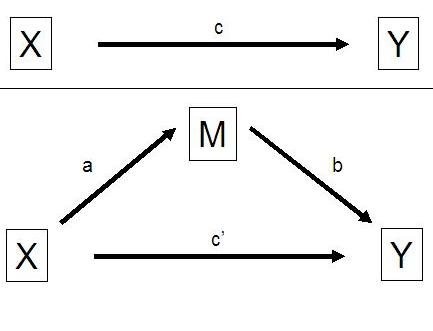
\includegraphics[scale = .5]{images/mediation_image.jpg}
    \caption{Mediation Analysis: direct and indirect effects}
    \label{fig:mediationAnalysis}
  \end{center}
\end{figure}

Mediation analysis works by testing the extent to which the variance in the outcome attributable to a predictor variable (the direct effect, or path ``c'': $Y_i \sim d_Y + cX_i + e_i$) can be explained \textit{indirectly} by the variance of two other relationships: that of the predictor variable and a third mediator (X $\rightarrow$ M, or path ``a")  and M and the outcome variable (path ``b''), controlling for the direct relationship between X and Y (path ``'c'') (see Figure ~\ref{fig:mediationAnalysis}). The mediation model can thus be denoted by two equations:

\begin{equation}
  M_i \sim d_M + aX_i + e_Mi
\end{equation}

\begin{equation}
  Y_i \sim d_Y + bM_i + c'X_i +  + e_{Yi}
\end{equation}
\bigskip

When combined, these two equations enable the calculation of the ``indirect effect'' of the predictor on the outcome, by controlling for the relationship between the mediator's effect on the outcome variable as a function of its relationship to the predictor variable.  While the direct effect measures the extent to which the dependent variable changes when the independent variable increases by one unit and the mediator variable remains unaltered, the indirect effect measures the extent to which the dependent variable changes when the independent variable is held fixed and the mediator variable changes by the amount it would have changed had the independent variable increased by one unit \citep{Bauer2006}.

The multilevel structure of the data in this study, i.e. the clustering of residuals according to team affiliation, violates the independence assumption of mediation analysis. As such, traditional multiple linear regression and path analysis will produce biased tests of the effects in the mediation model \citep{Raudenbush2002}.
%(Hox, 2002; Kreft & de Leeuw, 1998; Raudenbush & Bryk, 2002).
A multilevel mediation analysis must therefore additionally take into account variance attributable to the random effects of the model (team, in this case), and in so doing capture heterogeneity of variance in the indirect effect due to the level 2 variable \citep{Tofighi2014}.  To do this, each coefficient in the model must be random (denoted by subscript ``j''), so that the value of the coefficient varies across Level 2 units (team): \\

\begin{equation}
  M_{ij} \sim d_{Mj} + a_jX_{ij} + e_{Mij}
\end{equation}

\begin{equation}
  Y_{ij} \sim d_{Yj} + b_jM_{ij} + 'c_jX_{ij} +  + e_{Yij}
\end{equation}
\bigskip

Linear mixed effects regression models are fitted according to these equations, and estimates of mediation effects can be computed from these model parameters.  Subsequent mediation analyses were conducted using the ``mediation'' function of the Causal Mediation Analysis Package (version 4.4.5) in R.





\subsection{Post-Tournament Results}
For the following analyses, multilevel linear models were fit with Maximum Likelihood parameter estimation method using the lme4 package (Bates and Sarkar, 2006) in the R environment (R Development Core Team, 2006).  Team was included as a random effect, which allowed the intercepts and slopes of the response to vary according to team (i.e., random intercept model, see \citep{Pinheiro2000}; for an application, see \citep{Oberauer2006}). This helped statistically account for the intra-class correlation of observations within teams. Control and moderator variables were introduced into the model as fixed effects in a stepwise fashion, and model fit was judged by comparing the Akaike Information Criteria (AIC) and Bayesian Information Criteria (BIC) using a chi-squared test based on -2Log Likelihood score when possible.\footnote{The chi-squared test based on -2Log Likelihood scores was not possible when comparing models with different sample sizes.
This created difficulty when introducing covariates into the model, and subsequently reducing the number of observations} In addition, marginal and conditional $R^2$ values of equivalent models were compared and used as an indication of model effect size.\footnote{Nakagawa and Schielzeth (2013) have proposed a formula for calculating the proportion of variance explained by the fixed factor of the model (marginal $R^2$, compared to an intercept-only or null model), and the proportion of variance explained by the combination of the fixed factor plus the random factor, (conditional $R^2$, compared to the null)}





\subsubsection{1.a: Joint Action Success predicts Team Click}

In order to test the prediction that perceptions of joint-action success are positively related to team click in the post-Tournament data, the following model was constructed:

\begin{equation}
  \begin{align*}
    Team Click =  & Joint Action Success\\
              & + Individual Performance Success \\
              & + Objective Competence + Subjective Competence\\
              & + TournamentPerformanceMeasures \\
  \end{align*}
\end{equation}
\bigskip


Did perceptions of success in joint-action predict feelings of team click?  The model revealed a significant positive effect of Joint Action Success on Team Click, $\beta = .69$ ($95\% CI =  0.46, 0.89$), $SE = 0.11$, $t(13.23) = 6.20$, $p < .01$, $marginal R^2 = .53$, $conditional R^2 = .60$\footnote{Team was specified as a random effect, which allowed the slope and intercept of team click responses to vary by team. The predictor variable (Joint Action Success), moderator variables (Objective Competence and Subjective Competence), and controls (Individual Performance Success and Tournament performance measures) were introduced incrementally as fixed effects. To avoid issues of multicolinearity, Total Win Loss was excluded from the model, given the high pairwise correlation with Final Rank (.90). Pairwise correlation between all other predictor variables in the model was below .80}  Perceptions of success in individual performance components ($\beta = -.03$, $SE = .09$, $t(97) = -.33$, $p = .74$), objective ($\beta = .05$, $SE = .08$, $t(84.41) = .61$, $p = .54$) and subjective competence ($\beta = .11$, $SE = .07$, $t(87.76) = 1.57$, $p = .12$), and Tournament performance measures (Final Rank: $\beta = .02$, $SE = .04$, $t(92.85) = .58$, $p = .57$; Total Minutes: $\beta = .01$, $SE = .003$, $t(88.68) = 1.84$, $p = .07$), and Total Points: $\beta = .004$, $SE = .005$, $t(88.39) = .89$, $p = .38$)) did not significantly predict team click.  The inclusion of these fixed effects in the model did, however, significantly improve the overall model fit, as indicated by a comparison of AIC/BIC values between interactions of the model (see Table ~\ref{tab:MLM1aJointActionSuccessClick}).  Model residuals were normally distributed around zero ($W = 0.97, p = .03$), and individual cases had low influence on the model (Cook's Distances all < .25, see Appendix Figure ~\ref{fig:MLM1aAssumptions}). Results of this model support the prediction that athletes' perceptions of joint-action success correlate positively with feelings of ``team click.''


\begin{table}
\begin{center}
\begin{tabular}{l c c c }
\toprule
 & Intercept & Main effect & Controls \\
\midrule
(constant)                                                & $-0.04$  & $0.02$                & $-0.55$               \\
                                                          & $(0.15)$ & $(0.07)$              & $(0.37)$              \\
Team Performance Components                               &          & $\mathbf{0.65}^{***}$ & $\mathbf{0.66}^{***}$ \\
                                                          &          & $(0.10)$              & $(0.11)$              \\
Ind Performance Components                                &          &                       & $-0.04$               \\
                                                          &          &                       & $(0.09)$              \\
Objective Competence                                      &          &                       & $0.05$                \\
                                                          &          &                       & $(0.08)$              \\
Subjective Competence                                     &          &                       & $0.11$                \\
                                                          &          &                       & $(0.07)$              \\
Final Rank                                                &          &                       & $0.03$                \\
                                                          &          &                       & $(0.04)$              \\
Minutes Total                                             &          &                       & $0.00$                \\
                                                          &          &                       & $(0.00)$              \\
Points Total                                              &          &                       & $0.00$                \\
                                                          &          &                       & $(0.01)$              \\
Fatigue                                                   &          &                       & $0.10$                \\
                                                          &          &                       & $(0.08)$              \\
Extraverted                                               &          &                       & $0.03$                \\
                                                          &          &                       & $(0.05)$              \\
\midrule
AIC                                                       & 299.06   & 237.51                & 211.70                \\
BIC                                                       & 307.37   & 254.14                & 247.75                \\
Log Likelihood                                            & -146.53  & -112.76               & -91.85                \\
Num. obs.                                                 & 118      & 118                   & 97                    \\
\bottomrule
\multicolumn{4}{l}{\scriptsize{Coefficients with $p < 0.05$ in \textbf{bold}. Marginal $R^2 = .56$, Conditional $R^2 = .61$}}
\end{tabular}
\caption{Prediction 1: Team Performance Components predicts Team Click in the Post-Tournament survey data.}
\label{tab:MLM1aJointActionSuccessClick}
\end{center}
\end{table}





\subsubsection{1.b Team Performance Expectations predict Team Click}

To assess the prediction that more positive violation of expectations around team performance correlates with higher levels of team click, the following model was constructed:

\begin{equation}
  \begin{align*}
    Team Click =  & Team Performance Expectations \\
              &+ Individual Performance Expectations \\
              &+ Objective Competence + Subjective Competence \\
              &+ Tournament performance measures \\
  \end{align*}
\end{equation}

Expectations around individual performance, objective and subjective competence, and Tournament performance measures were introduced to the model as controls (fixed effects), while team was introduced as a random (level 2) effect.

Results of the model revealed a significant positive relationship between Team Performance Expectations and Team Click, $\beta = .52$ ($95\% CI =  0.28, 0.73$), $SE = 0.12$, $t(4.23) = 4.23$, $p < .001$, $marginal R^2 = .40$, $conditional R^2 = .56$.
Expectations around individual performance ($\beta = .04$, $SE = .08$, $t(86.26) = .46$, $p = .65$), objective ($\beta = .01$, $SE = .09$, $t(84.89) = .13$, $p = .89$) and subjective competence ($\beta = .12$, $SE = .07$, $t(91) = 1.62$, $p = .11$), and Tournament performance measures (Final Rank: $\beta = .08$, $SE = .05$, $t(44.33) = 1.72$, $p = .09$;
Total Minutes: $\beta = .004$, $SE = .003$, $t(87.05) = 1.00$, $p = .32$); Total Points: $\beta = .001$, $SE = .005$, $t(84.94) = .21$, $p = .84$)) did not significantly predict team click.  The inclusion of these effects did, however, improve the model fit, as indicated by the reduced AIC and increased marginal $R^2$ value (see Appendix Table ~\ref{tab:MLM1bteamExpectationsClick} for the various iterations of the model).  Model residuals were normally distributed around zero ($W = 0.98, p = .30$), and individual cases had low influence on the model (Cook's Distances all < .25, see Appendix Figure ~\ref{fig:MLM1bAssumptions}).  These results provide support for the prediction that more positive violations of expectations around team performance predict feelings of team click.



\begin{table}
\begin{center}
\begin{tabular}{l c c c }
\toprule
 & Intercept & Main effect & Controls \\
\midrule
(constant)                                 & $-0.04$  & $-0.00$               & $\mathbf{-0.79}^{*}$  \\
                                           & $(0.15)$ & $(0.09)$              & $(0.40)$              \\
Team Performance Vs Expectations           &          & $\mathbf{0.50}^{***}$ & $\mathbf{0.51}^{***}$ \\
                                           &          & $(0.11)$              & $(0.12)$              \\
Ind Performance Vs Expectations            &          &                       & $0.02$                \\
                                           &          &                       & $(0.08)$              \\
Objective Competence                       &          &                       & $0.02$                \\
                                           &          &                       & $(0.08)$              \\
Subjective Competence                      &          &                       & $0.12$                \\
                                           &          &                       & $(0.07)$              \\
Final Rank                                 &          &                       & $\mathbf{0.09}^{*}$   \\
                                           &          &                       & $(0.05)$              \\
Minutes Total                              &          &                       & $-0.00$               \\
                                           &          &                       & $(0.00)$              \\
Points Total                               &          &                       & $0.00$                \\
                                           &          &                       & $(0.01)$              \\
Fatigue                                    &          &                       & $\mathbf{0.18}^{*}$   \\
                                           &          &                       & $(0.09)$              \\
Extraverted                                &          &                       & $0.06$                \\
                                           &          &                       & $(0.05)$              \\
\midrule
AIC                                        & 299.06   & 268.43                & 228.63                \\
BIC                                        & 307.37   & 285.06                & 264.68                \\
Log Likelihood                             & -146.53  & -128.22               & -100.32               \\
Num. obs.                                  & 118      & 118                   & 97                    \\
Num. groups: team                          & 15       & 15                    & 14                    \\
\bottomrule
\multicolumn{4}{l}{\scriptsize{Coefficients with $p < 0.05$ in \textbf{bold}. Marginal $R^2 = .40$, Conditional $R^2 = .56$}}
\end{tabular}
\caption{Prediction 5: Team Performance Vs Expectations predicts Team Click in the Post-Tournament survey data (n = 97).}
\label{tab:MLM1bteamExpectationsClick}
\end{center}
\end{table}


\subsubsection{1.c Team Performance Expectations moderates the effect of Joint Action Success on team Click}

If both perceptions of joint-action success and positive violations of expectations predict team click, do these two predictors interact to predict click? Is team click higher for individuals whose perceived success in joint action was also a more positive violation of performance expectation? To test this possibility, the interaction term (Joint Action Success \times Team Performance Expectations) was included in model 1a as follows::

\begin{equation}
  \begin{align*}
    Team Click =  & Joint Action Success \times Team Performance Expectations \\
              &+ Individual Performance Success \\
              &+ Individual Performance Expectations \\
              &+ Objective Competence + Subjective Competence  \\
              &+ Tournament performance measures \\
  \end{align*}
\end{equation}
\bigskip
The inclusion of the interaction term failed to improve upon the fit of the previous model, judging by the relative goodness of fit, $AIC(1.c) = 217.91$ compared to $AIC(1.a) = 209.48$, $SD = .52 $, $\chi^2(18, N = 97) = 3.56$, $ p =.74$.  Results revealed that the interaction between Joint Action Success and Team Performance Expectations was not significant, $\beta = .002$ ($95\% CI =  -0.0062, 0.0063$), $SE = 0.08$, $t(39.7) = .026$, $p = .98$, $marginal R^2 = .56$, $conditional R^2 = .65$ (see Appendix, Table ~\ref{tab:MLM1cPerformanceClickInteraction}).


%\textit{See appendix A for details about model assumptions}.
%\newpage
%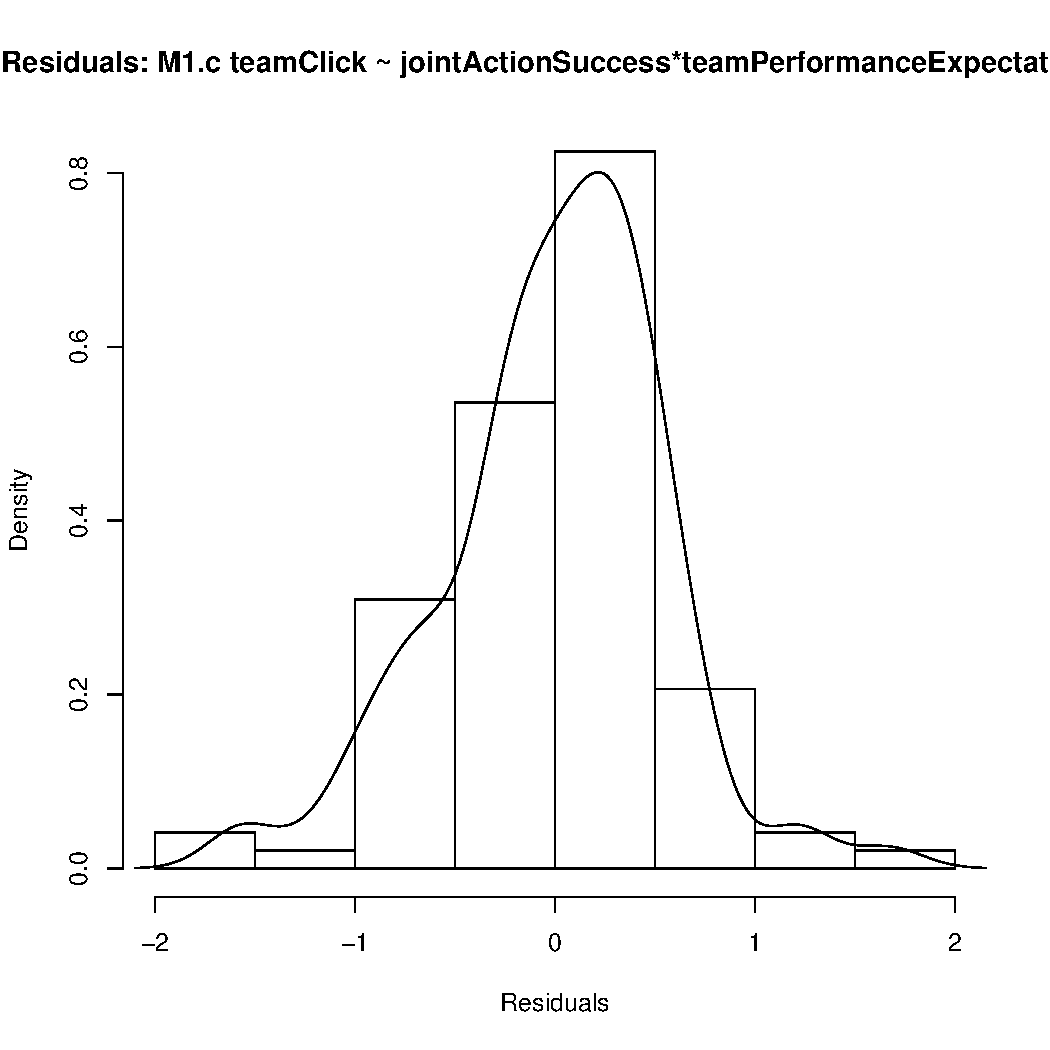
\includegraphics[scale =.4]{../images/MLM1cHist.pdf}
%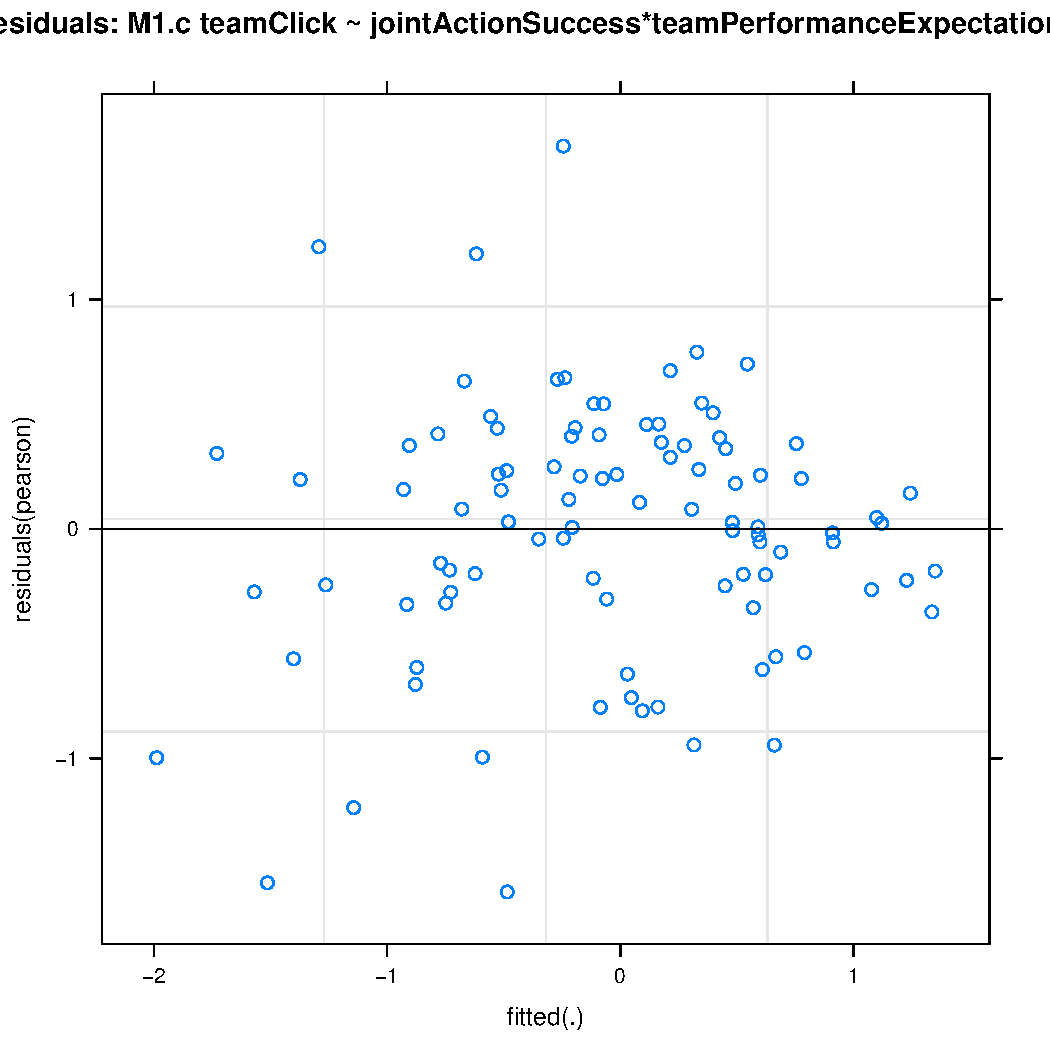
\includegraphics[scale =.4]{../images/MLM1cScatter.pdf}
%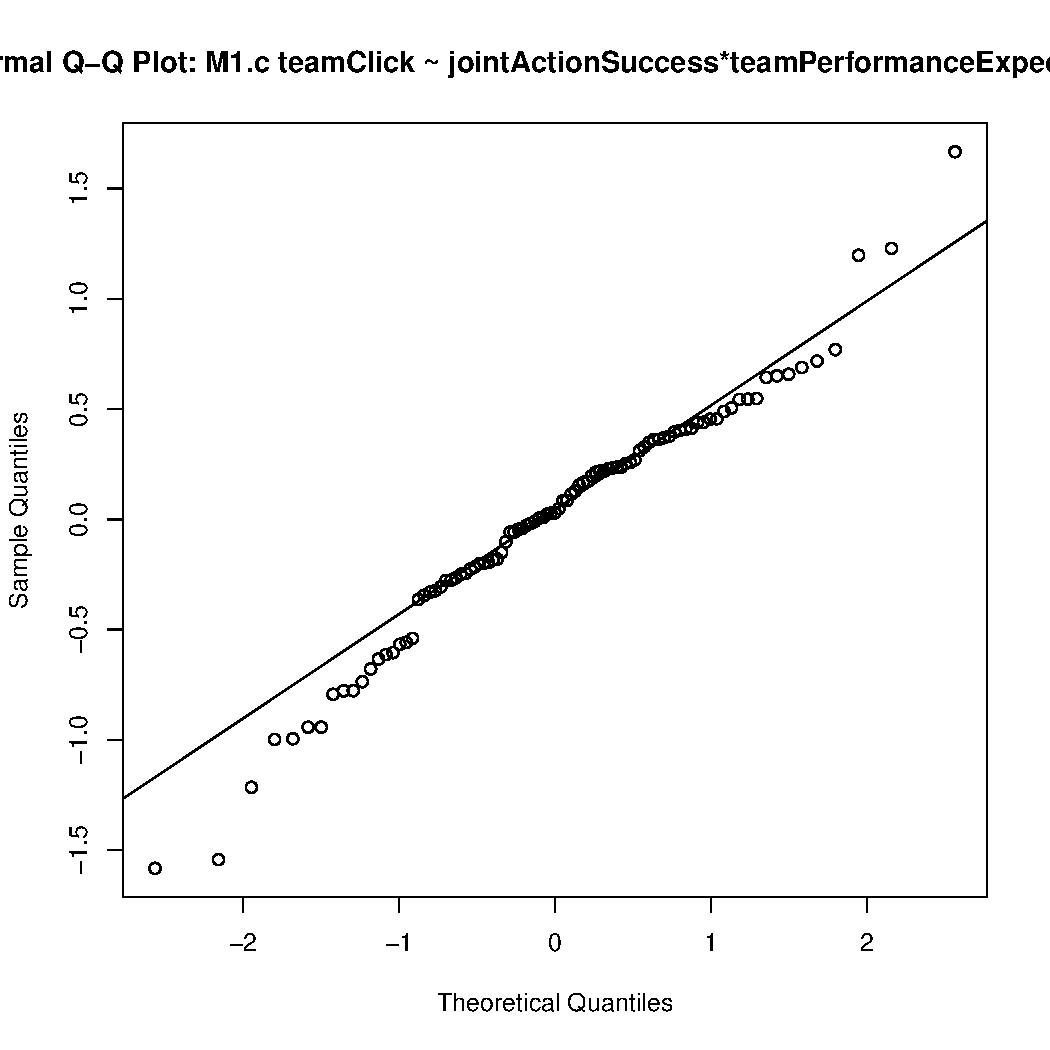
\includegraphics[scale =.4]{../images/MLM1cQQNorm.pdf}
%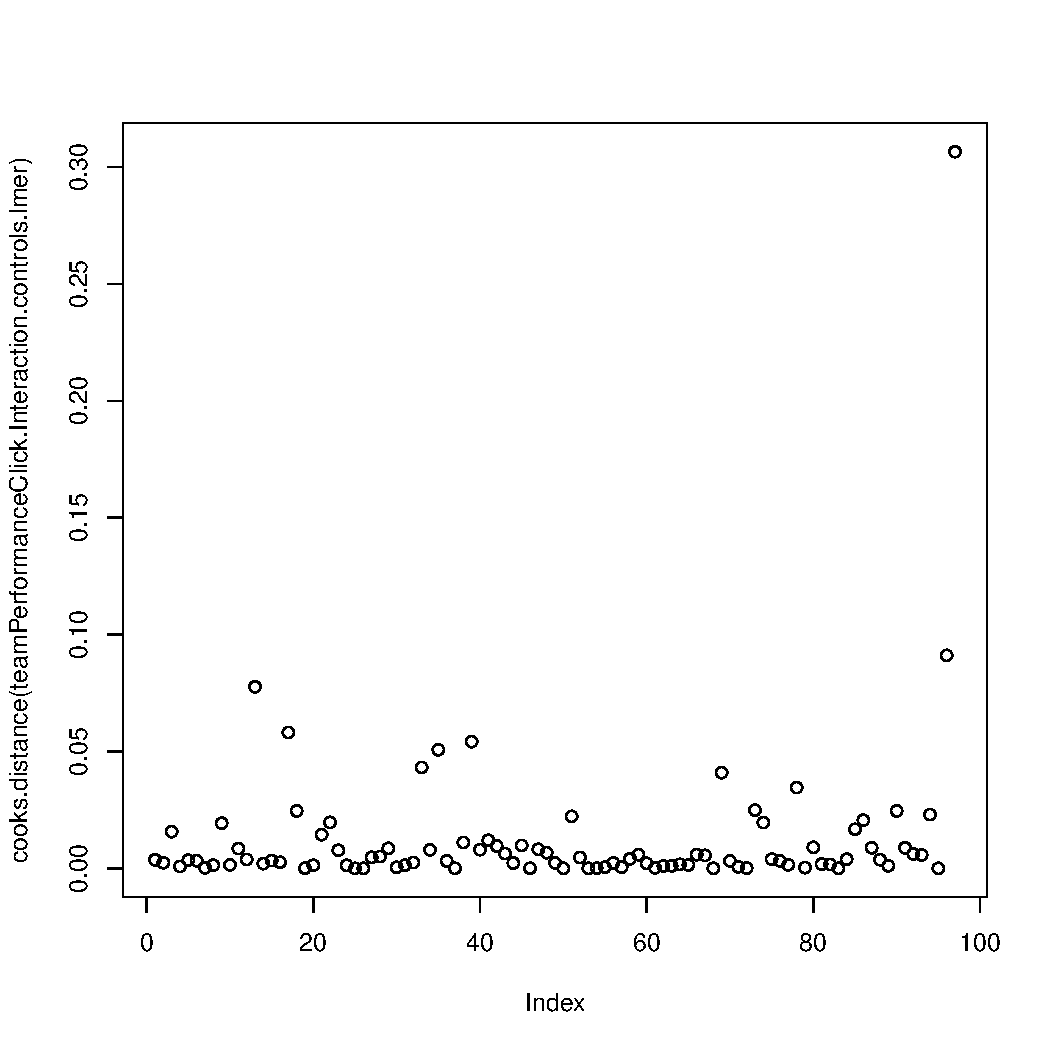
\includegraphics[scale =.4]{../images/MLM1cCooksD.pdf}

%\textit{problem here: increase in marginal and conditional R^2 values, perhaps due to adding additional variables into the model}
%The interaction did not improve the model fit,
%Nor did adding teamPerformance7 on its own into the model...
%But an interaction alone was significant

Findings from the first collection of models generally supported predictions. Team performance factors\nobreakdashperceptions of team component performance success and team performance relative to prior expectations\nobreakdashbut not individual performance factors significantly predicted team click, when controlling for subjective and objective competence, and Tournament performance measures.  The interaction effect of joint-action success and team performance expectations violation on team click was not significant.  Additionally, the low coefficient value for the model in which teamPerformanceExpectations predicted team click was low, indicating that this result should be treated with some caution.  Taken together, however, these results provide evidence for the predictions that perceptions of joint-action success is linked to feelings of team click.  Team performance expectations do not interact with perceptions of joint action to enhance feelings of team click, but rather function independently to predict team click, with those athletes who were experienced more positive violations of expectations also reporting higher levels of team click.






\subsubsection{2.a Team Click predicts Social Bonding}
The relationship between team click and social bonding was tested in the post-Tournament data. A linear mixed effects regression model was constructed with team as random effect, Team Click as fixed effect (predictor), and Social Bonding as outcome variable:

\begin{equation}
  \begin{align*}
    Social Bonding   =& Team Click\\
                    &+ Objective Competence + Subjective Competence  \\
                    &+ Tournament performance measures \\
  \end{align*}
\end{equation}
\bigskip

Controlling for Tournament performance measures and objective and subjective competence, the model revealed a significant relationship between team click and social bonding, $\beta = .67$ ($95\% CI =  .51, .84$), $SE = 0.08$, $t(16.01) = 8.22$, $p < .0001$, $marginal R^2 = .49$, $conditional R^2 = .51$ (see Table ~\ref{tab:MLM2aTeamClickBonding}).  Model residuals were normally distributed around zero ($W = 0.98, p = .15$), and individual cases had low influence on the model (Cook's Distances all < .15, see Appendix Figure ~\ref{fig:MKM2aAssumptions}).  This model supported the prediction that, following intense exertive joint-activity, higher levels of team click are associated with higher levels of social bonding.



% Table created by stargazer v.5.2 by Marek Hlavac, Harvard University. E-mail: hlavac at fas.harvard.edu
% Date and time: Mon, Jun 26, 2017 - 20:48:41
\begin{table}[!htbp] \centering 
  \caption{socialBonding = teamClick} 
  \label{tab:MLM2aTeamClickBonding} 
\begin{tabular}{@{\extracolsep{5pt}}lccc} 
\\[-1.8ex]\hline 
\hline \\[-1.8ex] 
 & \multicolumn{3}{c}{\textit{Dependent variable:}} \\ 
\cline{2-4} 
\\[-1.8ex] & \multicolumn{3}{c}{socialBonding} \\ 
\\[-1.8ex] & (1) & (2) & (3)\\ 
\hline \\[-1.8ex] 
 (constant) & $-$0.01 & $-$0.0002 & 0.21 \\ 
  & (0.10) & (0.07) & (0.27) \\ 
  & & & \\ 
 teamClick &  & 0.64$^{***}$ & 0.67$^{***}$ \\ 
  &  & (0.08) & (0.08) \\ 
  & & & \\ 
 objectiveCompetence &  &  & 0.04 \\ 
  &  &  & (0.08) \\ 
  & & & \\ 
 subjectiveCompetence &  &  & 0.12 \\ 
  &  &  & (0.07) \\ 
  & & & \\ 
 finalRank &  &  & $-$0.01 \\ 
  &  &  & (0.04) \\ 
  & & & \\ 
 minutesTotal &  &  & $-$0.003 \\ 
  &  &  & (0.004) \\ 
  & & & \\ 
 pointsTotal &  &  & $-$0.002 \\ 
  &  &  & (0.01) \\ 
  & & & \\ 
\hline \\[-1.8ex] 
Marginal R-squared &  &  & .49 \\ 
Conditional R-squared &  &  & .51 \\ 
Observations & 118 & 118 & 97 \\ 
Log Likelihood & $-$151.95 & $-$118.76 & $-$97.75 \\ 
Akaike Inf. Crit. & 309.90 & 249.53 & 217.50 \\ 
Bayesian Inf. Crit. & 318.21 & 266.15 & 245.82 \\ 
\hline 
\hline \\[-1.8ex] 
\textit{Note:}  & \multicolumn{3}{r}{$^{*}$p$<$0.05; $^{**}$p$<$0.01; $^{***}$p$<$0.001} \\ 
\end{tabular} 
\end{table} 





\subsubsection{3.a Joint Action Success predicts Social Bonding}

In light of evidence for significant relationships between joint-action success and team click, and team click and social bonding, the direct relationship between joint-action success and social bonding was assessed. Controlling for perceptions of success in individual performance, objective and subjective competence, and Tournament performance measures, the model revealed a significant effect of joint-action success on social bonding, $\beta = .45$ ($95\% CI =  .17, .73$), $SE = .14$, $t(23.4) = 3.19$, $p < .01$, $marginal R^2 = .27$, $conditional R^2 = .42$.  The model also revealed a significant positive effect of subjective measures of competence on social bonding, $\beta = .18$ ($95\% CI =  .03, .35$), $SE = .08$, $t(90.86) = 2.26$, $p = .03$ (full results in Table ~\ref{tab:MLM3aJointActionSuccessBonding}).

While Levene's Test for Equality of Variance indicated that the assumption of homoscedasticity was met at the group-level, $F(13,83) = .80, p = .66$, overall model residuals were non-normally distributed ($W = 0.95, p = .0007$), owing to relatively large negative skew (-.87) (see Appendix Figure ~\ref{fig:MLM3aAssumptions}). Non-normally distributed residuals are problematic as they may influence the model's ability to generate accurate parameter estimates . Two data manipulation techniques were considered in order to normalise residuals and therefore preserve the estimates of the model: exclusion of outliers and transformation of the outcome variable.  Transformation of the outcome variables was the preferred method over outlier exclusion, due to the cost involved in removing observations that may be of potential theoretical relevance to the scientific investigation \citep{Rousseeuw2011}. Nonetheless, for this first phase of analysis, both outlier exclusion and transformation manipulations of the data were performed and reported.

Exclusion of outliers according to Tukey's method (observations above and below 1.5x the Inter Quartile Range (IQR), see \citep{Tukey1977}) appeared to improve the model fit, $\beta = .26$ ($95\% CI =  .05, .47$), $SE = 0.004$, $t(9.78) = 3.66$, $p < .01$, $marginal R^2 = .18$, $conditional R^2 = .34$.
The distribution of model residuals appeared to improve, but still violated the assumption of normality ($Shapiro-Wilk = 0.96, p = .009$).  Individual cases had low influence on the model (Cook's Distances all < .10).

Due to the \textit{positive} skew of the model residuals, the outcome variable was transformed by taking the log of the reversed scores of the outcome variable, i.e. $log10(k - y)$, where $k$ is a constant value from which each score for $y$ is subtracted so that the distribution of the outcome variable is reversed\citep{Howell2012}.\footnote{Reversing the distribution of the outcome variable allows the logarithmic function to normalise the distribution of the variable, by pushing them from the left hand side of the distribution towards the centre}  Transformed values were then returned to their original direction for analysis\citep{Field2012}.  Rebuilding the model with a log-transformed outcome variable appeared to improve the fit of the model more than the outlier-removed model, and avoided the removal of any observations.
The distribution of residuals appeared more normal, ($W = 0.97, p = .04$), and the R-squared values for the model improved, $marginal R^2 = .27$, $conditional R^2 = .43$ (see Table ~\ref{tab:MLM3aJointActionSuccessBonding} for results of all three models, and Appendix Figures ~\ref{fig:MLM3aAssumptions}\nobreakdash~\ref{fig:MLM3aLogAssumptions}).  Results of the log-transformed model indicated that the non-normally distributed residuals of the original model did not impact the estimates of the model. As such, the results of these models were taken as evidence for a significant positive relationship between perceptions of joint-action success and feelings of social bonding.


% Table created by stargazer v.5.2 by Marek Hlavac, Harvard University. E-mail: hlavac at fas.harvard.edu
% Date and time: Mon, Jun 26, 2017 - 21:18:41
\begin{table}[!htbp] \centering 
  \caption{socialBonding = jointActionSuccess} 
  \label{tab:MLM3aJointActionSuccessBonding} 
\footnotesize 
\begin{tabular}{@{\extracolsep{5pt}}lccc} 
\\[-1.8ex]\hline 
\hline \\[-1.8ex] 
 & \multicolumn{3}{c}{\textit{Dependent variable:}} \\ 
\cline{2-4} 
\\[-1.8ex] & socialBonding & bondingPostFactorOut & bondingPostFactorLogReturned \\ 
 &  & outliers removed & log-transformed \\ 
\\[-1.8ex] & (1) & (2) & (3)\\ 
\hline \\[-1.8ex] 
 (constant) & $-$0.06 & $-$0.06 & 1.97$^{***}$ \\ 
  & (0.31) & (0.31) & (0.13) \\ 
  & & & \\ 
 jointActionSuccess & 0.45$^{**}$ & 0.45$^{**}$ & 0.20$^{***}$ \\ 
  & (0.14) & (0.14) & (0.06) \\ 
  & & & \\ 
 indPerformanceSuccess & 0.05 & 0.05 & $-$0.001 \\ 
  & (0.11) & (0.11) & (0.05) \\ 
  & & & \\ 
 objectiveCompetence & 0.07 & 0.07 & 0.04 \\ 
  & (0.10) & (0.10) & (0.04) \\ 
  & & & \\ 
 subjectiveCompetence & 0.19$^{*}$ & 0.19$^{*}$ & 0.09$^{*}$ \\ 
  & (0.08) & (0.08) & (0.03) \\ 
  & & & \\ 
 finalRank & $-$0.02 & $-$0.02 & $-$0.01 \\ 
  & (0.05) & (0.05) & (0.02) \\ 
  & & & \\ 
 minutesTotal & 0.002 & 0.002 & 0.001 \\ 
  & (0.004) & (0.004) & (0.002) \\ 
  & & & \\ 
 pointsTotal & $-$0.001 & $-$0.001 & $-$0.002 \\ 
  & (0.01) & (0.01) & (0.003) \\ 
  & & & \\ 
\hline \\[-1.8ex] 
Marginal R-squared & .27 & .18 & .28 \\ 
Conditional R-squared & .42 & .34 & .43 \\ 
Observations & 97 & 97 & 97 \\ 
Log Likelihood & $-$113.05 & $-$113.05 & $-$29.49 \\ 
Akaike Inf. Crit. & 250.10 & 250.10 & 82.98 \\ 
Bayesian Inf. Crit. & 281.00 & 281.00 & 113.87 \\ 
\hline 
\hline \\[-1.8ex] 
\textit{Note:}  & \multicolumn{3}{r}{$^{*}$p$<$0.05; $^{**}$p$<$0.01; $^{***}$p$<$0.001} \\ 
\end{tabular} 
\end{table} 



\subsubsection{3.b Team Performance Expectations predicts Social Bonding} % very small effect

The direct relationship between expectations around team performance and social bonding was also tested.  The model revealed a significant positive relationship between Team Performance Expectations and Social Bonding, $\beta = .34$ ($95\% CI =  .06, .63$), $SE = .14$, $t(13.79) = 2.38$, $p = .03$, $marginal R^2 = .20$, $conditional R^2 = .40$.  The model also revealed a significant positive effect of Subjective Competence on Social Bonding, $\beta = .19$ ($95\% CI =  .02, .36$), $SE = .08$, $t(90.37) = 2.24$, $p = .03$, such that athletes who provided higher ratings of their own technical competence in rugby (measured before the Tournament) reported higher levels of social bonding.

Model residuals were not normally distributed, ($W = 0.91, p < .0001$), owing to large negative skew ($-1.33$) and high kurtosis ($.49$). Re-running the model with a log-transformed outcome variable appeared to make the best improvement to model residuals more than the outlier-removed model (see Table ~\ref{tab:MLM3bExpectationsBonding}). In the log-transformed model, the distribution of model residuals appeared most normal,  ($W = 0.97, p = .02$), and the R-squared values for the model improved, $marginal R^2 = .23$, $conditional R^2 = .44$.  Individual cases had low influence on the model (Cook's Distances all < .15, see Appendix Figures ~\ref{fig:MLM3bAssumptions} and ~\ref{fig:MLM3bLogAssumptions} for a comparison of model assumptions between the original and log-transformed model). Owing to non-normally distributed residuals, this model does not provide robust support for the prediction that team performance expectation violations relates directly to social bonding.

Results outlined above demonstrate significant relationships between Joint-Action Success and Team Click, Team Click and Social Bonding, and a direct relationship between Joint-Action Success and Social Bonding. Results of models linking Team Performance Expectations, Team Click, and Social Bonding were lest robust, and should be treated with caution.


%Outlier exclusion
%Exclusion of outliers improved the distribution of residuals, ($W = 0.96, p = .007$), and individual cases had low influence on the model (Cook's Distances all < .15).  The significant positive effect of teamPerformanceExpectations on socialBonding remained in the adjusted model, $\beta = .01$ ($95\% CI =  .003, .02$), $SE = .004$, $t() = 2.65$, $p = .03$, $marginal R^2 = .19$, $conditional R^2 = .40$.  The effect of Subjective Competence on socialBonding was no longer significant, $\beta = .12$ ($95\% CI =  -.0004, .24$), $SE = .06$, $t(90.44) = 1.95$, $p = .06$.

\newgeometry{margin=0.5cm}

% Table created by stargazer v.5.2 by Marek Hlavac, Harvard University. E-mail: hlavac at fas.harvard.edu
% Date and time: Tue, Jun 27, 2017 - 17:01:54
\begin{table}[!htbp] \centering 
  \caption{M3.b socialBonding = teamPerformanceExpectations} 
  \label{tab:MLM3bExpectationsBonding} 
\scriptsize 
\begin{tabular}{@{\extracolsep{5pt}}lccc} 
\\[-1.8ex]\hline 
\hline \\[-1.8ex] 
 & \multicolumn{3}{c}{\textit{Dependent variable:}} \\ 
\cline{2-4} 
\\[-1.8ex] & socialBonding & bondingPostFactorOut & bondingPostFactorLogReturned \\ 
 &  & outliers removed & log-transformed \\ 
\\[-1.8ex] & (1) & (2) & (3)\\ 
\hline \\[-1.8ex] 
 (constant) & $-$1.67$^{*}$ & $-$1.18$^{*}$ & 1.19$^{***}$ \\ 
  & (0.73) & (0.53) & (0.31) \\ 
  & & & \\ 
 teamPerformanceExpectations & 0.01$^{*}$ & 0.01$^{**}$ & 0.01$^{**}$ \\ 
  & (0.01) & (0.004) & (0.003) \\ 
  & & & \\ 
 individualPerformanceExpectations & 0.004 & 0.001 & 0.001 \\ 
  & (0.004) & (0.003) & (0.002) \\ 
  & & & \\ 
 objectiveCompetence & 0.03 & 0.02 & 0.02 \\ 
  & (0.10) & (0.07) & (0.04) \\ 
  & & & \\ 
 subjectiveCompetence & 0.19$^{*}$ & 0.12 & 0.08$^{*}$ \\ 
  & (0.09) & (0.06) & (0.04) \\ 
  & & & \\ 
 finalRank & 0.08 & 0.10 & 0.04 \\ 
  & (0.13) & (0.09) & (0.05) \\ 
  & & & \\ 
 minutesTotal & 0.0003 & 0.001 & 0.0001 \\ 
  & (0.004) & (0.003) & (0.002) \\ 
  & & & \\ 
 pointsTotal & $-$0.04 & $-$0.06 & $-$0.03 \\ 
  & (0.09) & (0.06) & (0.04) \\ 
  & & & \\ 
 pointsTotal & $-$0.001 & $-$0.004 & $-$0.002 \\ 
  & (0.01) & (0.005) & (0.003) \\ 
  & & & \\ 
\hline \\[-1.8ex] 
Marginal R-squared & .20 & .19 & .23 \\ 
Conditional R-squared & .40 & .40 & .44 \\ 
Observations & 97 & 91 & 97 \\ 
Log Likelihood & $-$117.26 & $-$77.84 & $-$32.42 \\ 
Akaike Inf. Crit. & 260.52 & 181.67 & 90.85 \\ 
Bayesian Inf. Crit. & 293.99 & 214.31 & 124.32 \\ 
\hline 
\hline \\[-1.8ex] 
\textit{Note:}  & \multicolumn{3}{r}{$^{*}$p$<$0.05; $^{**}$p$<$0.01; $^{***}$p$<$0.001} \\ 
\end{tabular} 
\end{table} 

\restoregeometry



\subsubsection{4.a Mediation analysis: Joint Action Success predicts Social Bonding, mediated by Team Click}
Mediation analyses were conducted using linear mixed effects regressions in the Causal Mediation Analysis package in R (Version 4.4.5).  To make inferences concerning the average indirect and total effects, quasi-Bayesian Markov Chain Monte Carlo (MCMC) method based on normal approximation and 1000 simulations was used to estimate the 95\% Confidence Intervals \citep{Tofighi2016a,Imai2010}. MCMC estimation is a form of non-parametric bootstrapping whereby the sampling distribution for the effect of interest is not assumed to be normal but is instead simulated from the model estimates and their asymptotic variances and covariances \cite{Preacher2008}.

Results of the mediation analysis revealed significant average indirect effect of Joint Action Success on Social Bonding attributable to Team Click, $\beta = .37, 95\% CI = 0.20 , 0.59, p < .001$.  When controlling for the effect of team click on social bonding, the average direct effect between Joint Action Success and Social Bonding was no longer significant, $\beta = -.006, 95\% CI = -.27 , .23, p = .96 $ (see Figure ~\ref{fig:MLM4aMediationAnalysis}). The direct effect diminished such that including Joint Action Success in the model produced a total effect that was marginally \textit{smaller} than the indirect effect alone, $\beta = .36, 95\% CI = .13 , .61, p = .01$. These results suggest that feelings of team click fully mediate the relationship between perceptions of joint-action success and social bonding.


%Residuals of the mediation model were normally distributed around zero, ($W = 0.99, p < .28$, see Figure ~\ref{fig:MLM4aAssumptions} for model assumptions).



\subsubsection{4.b Mediation analysis: Team Performance Expectations predicts Social Bonding, mediated by Team Click}

Post-Tournament results also demonstrate a significant positive relationship between Team Performance Expectations and Team Click. The model generated for relationships between between Team Performance Expectations and Social Bonding, however, was not robust to the demands of model assumptions.   Nonetheless, mediation analysis was used to test the possibility that Team Click mediated the effects of Team Performance Expectations on Social Bonding.

Results of the mediation analysis revealed significant average indirect effect of Team Performance Expectations on Social Bonding attributable to Team Click, $\beta = .36, 95\% CI = 0.17 , 0.62, p < .0001$.  When controlling for the effect of Team Click on Social Bonding, the average direct effect between Team Performance Expectations and Social Bonding was no longer significant, $\beta = -.07, 95\% CI = -.27 , .12, p = .84 $ (see Figure ~\ref{fig:MLM4bMediationAnalysis}). The total effect of the model was significant $\beta = .29, 95\% CI = .02 , .57, p = .04$.  This model, as with model 4.a above, indicated that Team Click fully mediated the relationship between Team Performance Expectations and Social Bonding.


Again, the results of this mediation model should be treated with caution, given the fact that the mediation model is composed of a non-robust statistical model (i.e., path ```'c'').

\begin{figure}[htbp]
  \centering
  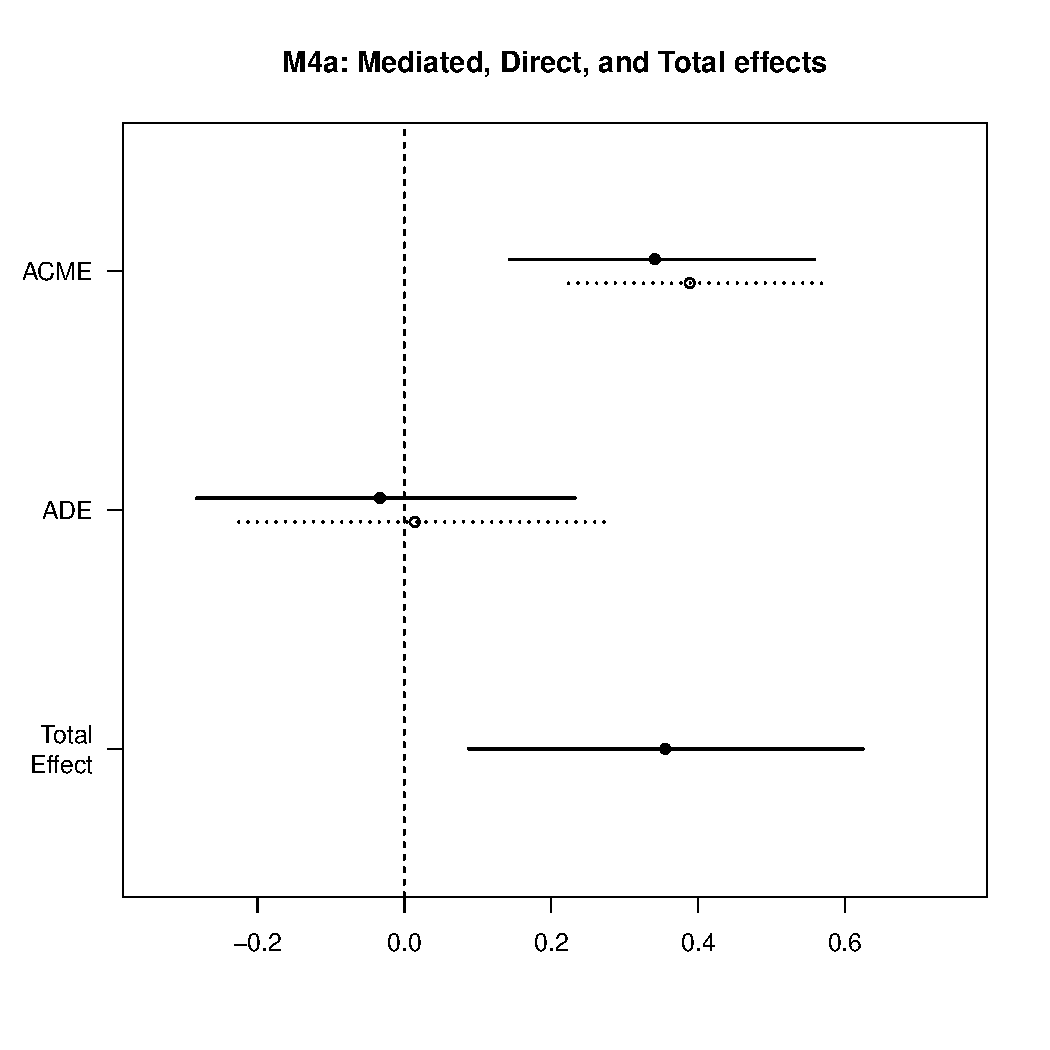
\includegraphics[scale = .5]{images/MLM4aMediationEffects.pdf}
  \caption{M4a Mediation Analysis}
  \label{fig:MLM4aMediationAnalysis}
\end{figure}

\begin{figure}[htbp]
  \centering
  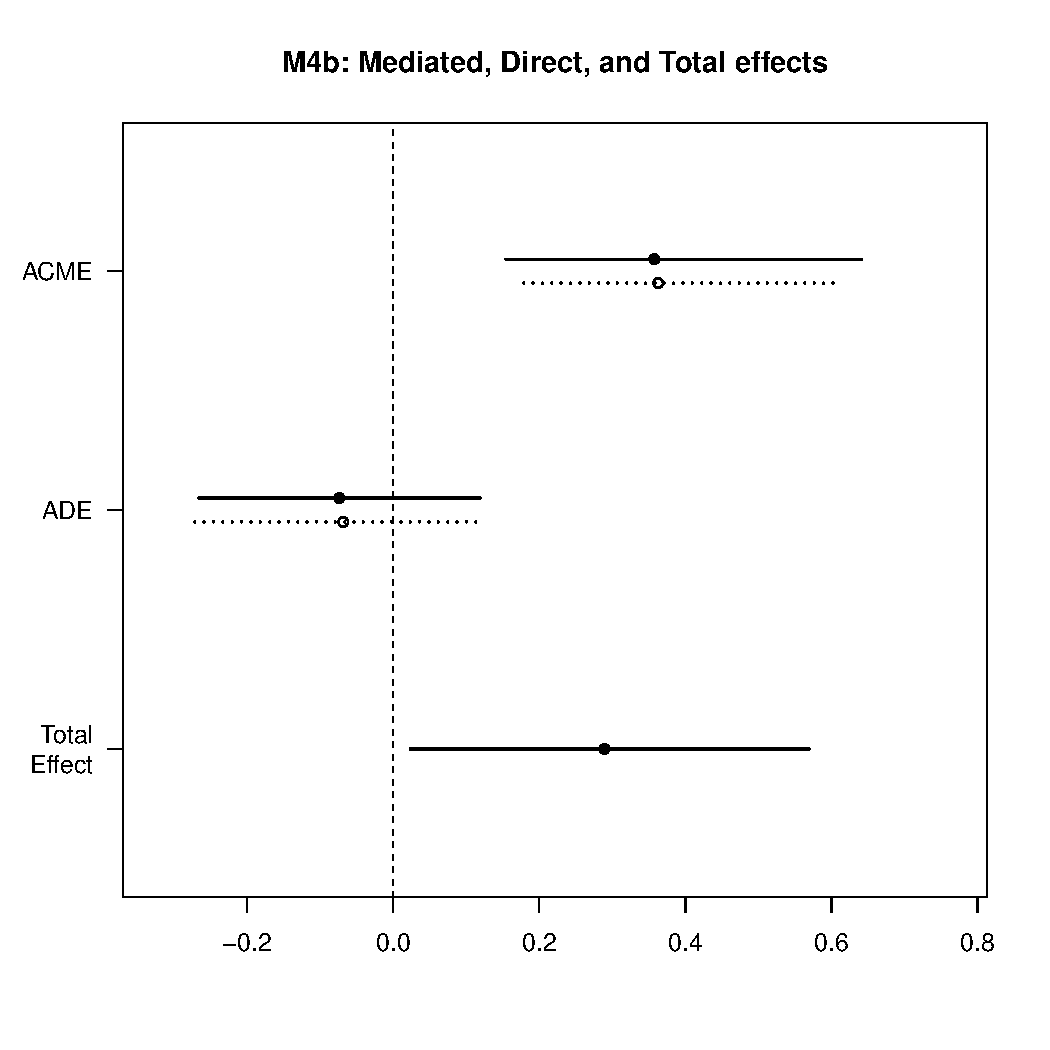
\includegraphics[scale = .5]{images/MLM4bMediationEffects.pdf}
  \caption{M4b Mediation Analysis}
  \label{fig:MLM4bMediationAnalysis}
\end{figure}





%\begin{figure}[htbp]
%  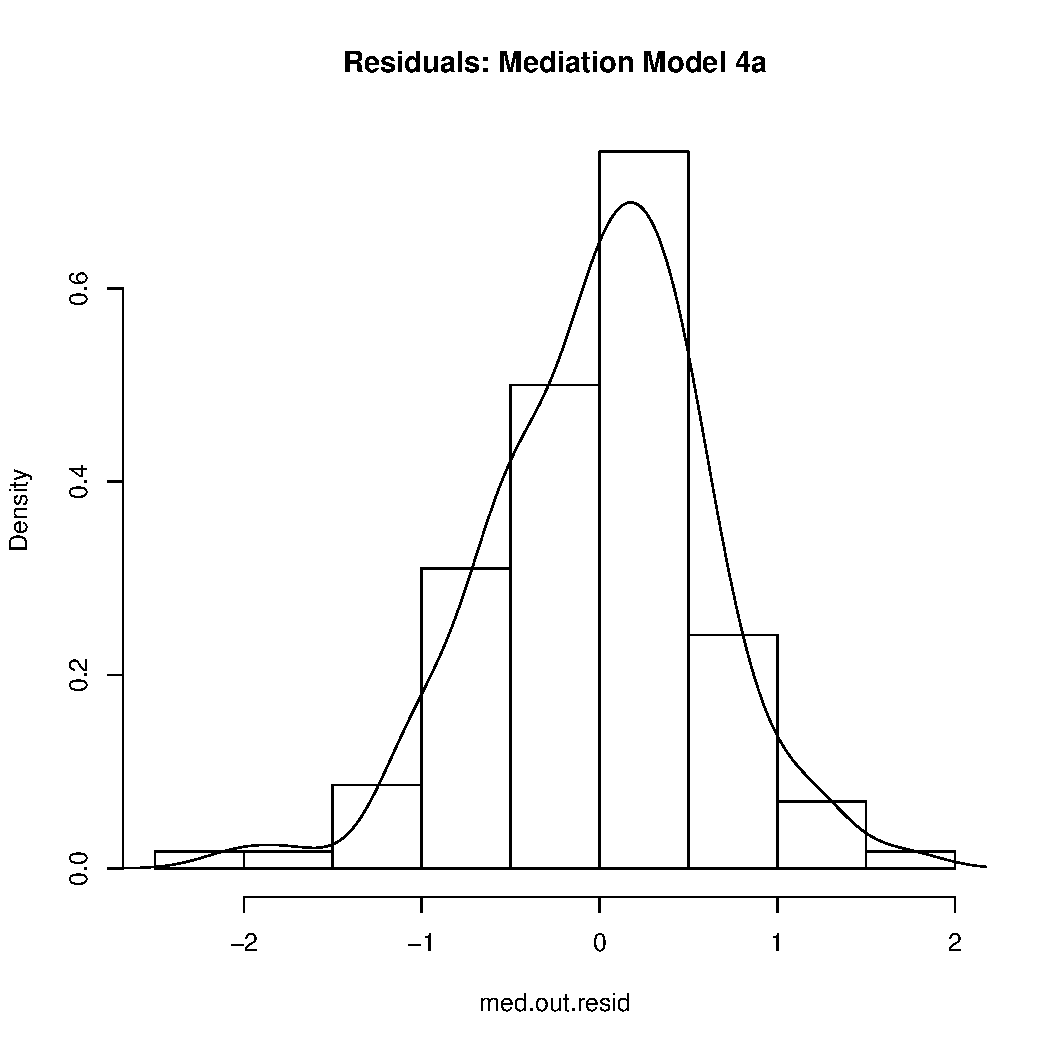
\includegraphics{finalDocuments/images/MLM4aResiduals.pdf}
%  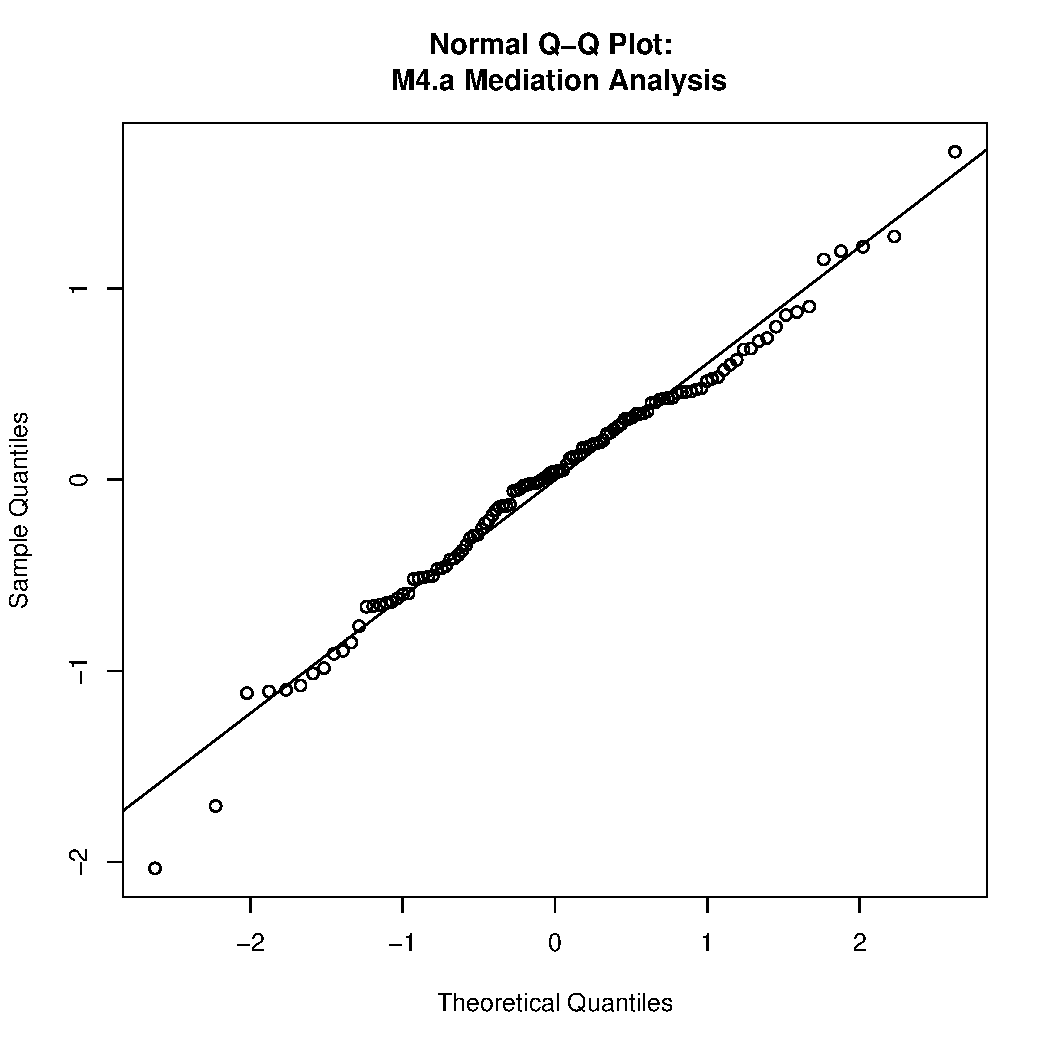
\includegraphics{finalDocuments/images/MLM4aQQNorm.pdf}
%  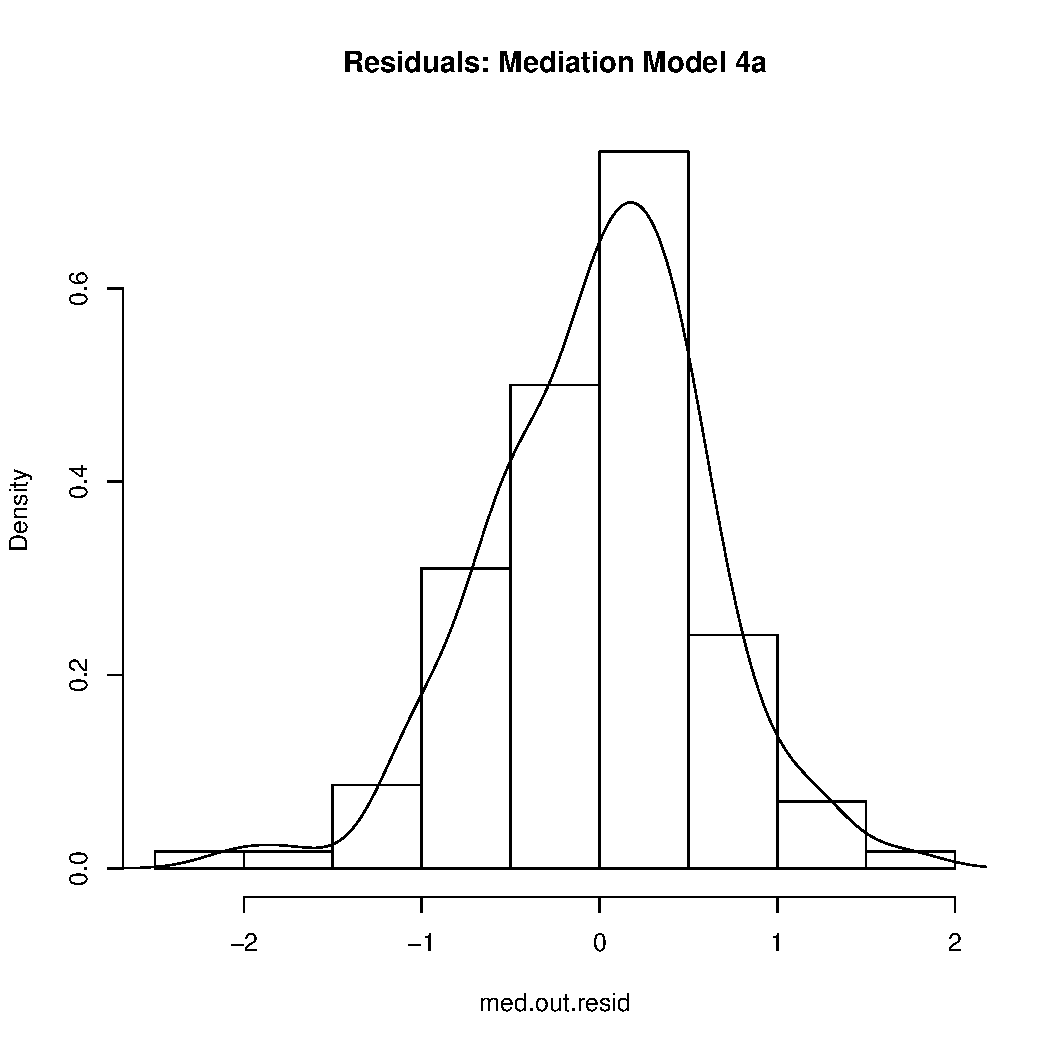
\includegraphics{finalDocuments/images/MLM4aResiduals.pdf}
%  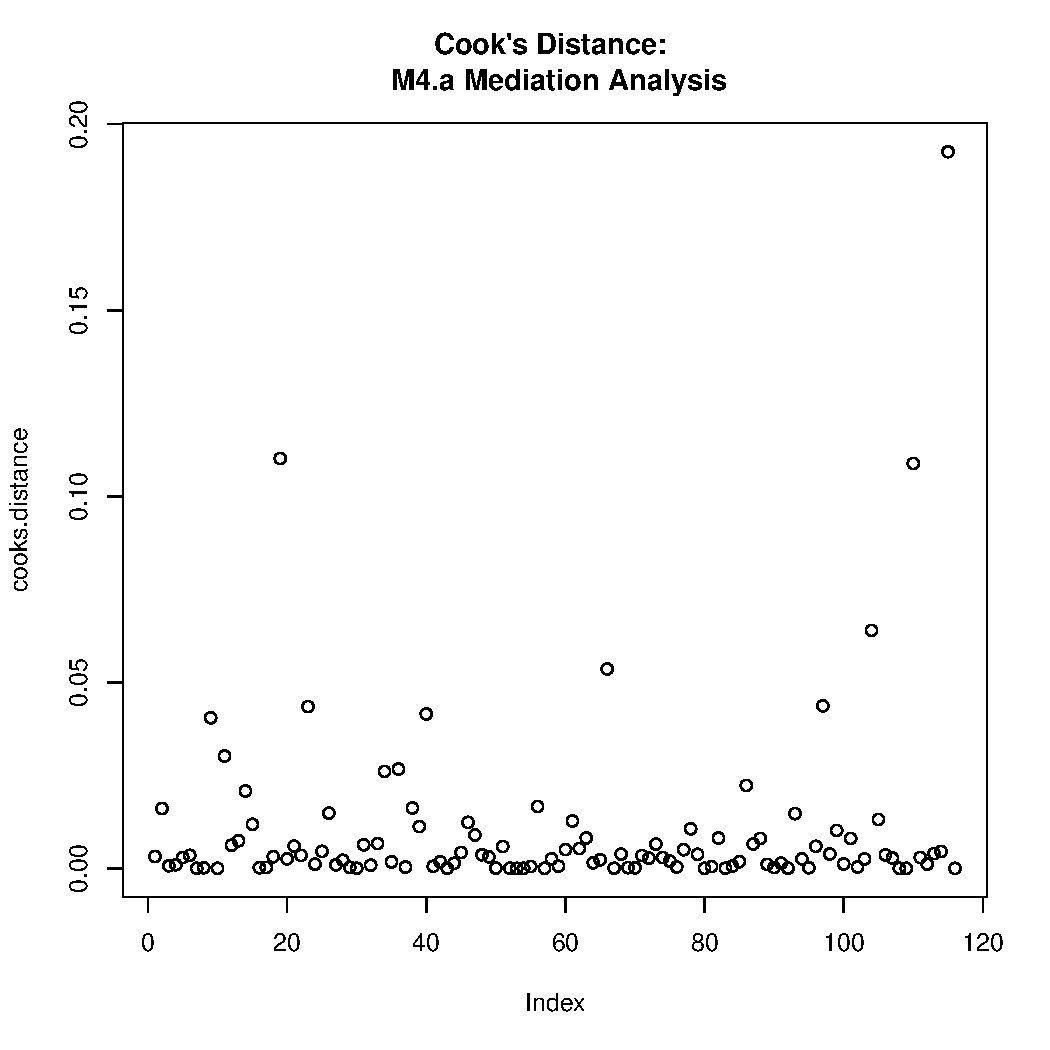
\includegraphics{finalDocuments/images/MLM4aCooksD.pdf}
%  \caption{M4a Mediation Analysis}
%  \label{fig:MLM4aAssumptions}
%\end{figure}

% (Baer et al 2006: 147) One method for constructing CIs assumes normality for the sampling distributions of the estimates. Under this assumption, 95% CIs for the average indirect effect and average total effect are obtained as Alternatively, one could perform a null hypothesis test by forming the critical ratio of each estimate to its standard error and comparing the result with the critical value of the z distribution. In andthe as- sumption of normality for the sampling distributions will not hold exactly, given that aˆb ˆ is a product of normally distributed estimates (and hence will not be normal). The deviation from normality may be small enough, however, that the CIs or significance tests will still be reasonably accurate.

%An alternative method for constructing CIs that may hold promise is the Monte Carlo (MC) method of MacKinnon et al. (2004). In this approach, the sampling distribution for the effect of interest is not assumed to be normal and is instead simulated from the model estimates and their asymptotic variances and covariances (a form of parametric bootstrap- ping). For instance, to simulate the sampling distribution of the average indirect effect, one would define a multinormal distribution with means equal to a ˆ, b ˆ, and ˆ aj ,bj and covariance matrix equal to the estimated covariance matrix of these estimates. One would then take random values from this multinormal distribution and plug them into Equation 5 to compute the average indirect effect. Collecting the results over many draws provides a simulated sampling distribution for the average indirect effect. One would then obtain conidence limits for the average indirect effect by taking the

%Preacher, K. J., & Selig, J. P. (2010, July). Monte Carlo method for assessing multilevel Mediation: An interactive tool for creating confidence intervals for indirect effects in 1-1-1 multilevel models [Computer software]. Available from http://quantpsy.org/.






\subsection{Discussion of Results: post-Tournament Analysis}
The results of the post-Tournament survey responses generally support predictions concerning the relationships between perceptions of joint action success, team click and social bonding.  The relationship between team performance expectations, team click, and social bonding, however, is less convincing.  Model 1.b, in which Team Performance Expectations predicts Team Click, while statistically significant, generates a very small beta coefficient.  Model 3.b, in which the relationship between Team Performance Expectations and Social Bonding, is not robust to model assumptions, and thus compromises the validity of the mediation analysis (model 4.b).  These results could suggest that while more positive violations of team performance expectations do contribute to feelings of Team Click, they might not contribute as strongly to feelings of social bonding.

Results show that, by contrast, perceived Joint Action Success is a strong predictor of both Team Click and Social bonding. Mediation analysis indicates that Team Click fully mediates the relationship between Joint Action Success and Social Bonding.


































\clearpage
\subsection{Analysis of pre-post Tournament data}
The predictions of the present study were further tested through an analysis of change in variables of interest between the pre- and post-Tournament surveys. By analysing pre- and post-Tournament responses, it was possible to investigate 1) to what extent variables of interest changed during the Tournament, and 2) whether pre-post changes in variables of interest were consistent with study predictions concerning the relationship between joint-action, team click, and social bonding.  When controlling for objective measures of success and feelings concerning individual performance, could change in social bonding be explained by changes in perceptions of joint-action success and/or changes in feelings of team click?




\subsubsection{Roadmap of pre-post Tournament Analysis}
Analysis of the pre-post Tournament data proceeded in the same manner as the post-Tournament data. The hypothesised relationship between joint-action success and social bonding was broken down into component relationships. \\

First, changes in feelings of team click were analysed as a function of changes in 1) perceptions of team component performance (Joint Action Success Pre Post), 2) post-Tournament appraisal of team performance relative to prior expectations (Team Performance Expectations), and 3) the interaction between these two predictor variables.
\bigskip
\begin{description}
  \item [Prediction 2.1.a] $\Delta$Joint Action Success  $\rightarrow$  $\Delta$Team Click
  \item [Prediction 2.1.b] $\Delta$Team Performance Expectations $\rightarrow$ $\Delta$ Team Click
  \item [Prediction 2.1.c] $\Delta$Joint Action Success $\rightarrow$ $\Delta$Team Click, moderated by $\Delta$Team Performance Expectations
\end{description}

Second, the change observed in social bonding (Social Bonding Pre Post) was analysed as a function of change in feelings of team click.
\bigskip
\begin{description}
  \item [Prediction 2.2.a] $\Delta$Team Click $\rightarrow$ $\Delta$Social Bonding
\end{description}

Third, the direct relationships between predictor variables (change in perceptions of join-action success and appraisal of team performance relative to prior expectation) and change in social bonding was analysed:
\bigskip
\begin{description}
  \item [Prediction 2.3.a] $\Delta$Joint Action Success $\rightarrow$ $\Delta$Social Bonding
  \item [Prediction 2.3.b] $\Delta$Team Performance Expectations $\rightarrow$ $\Delta$Social Bonding
\end{description}

Finally, a mediation analysis was performed to formally test whether feelings of team click mediated a direct relationship between perceptions of joint-action success and social bonding.

\begin{description}
  \item[Prediction 2.4.a Mediation Analysis] $\Delta$Joint Action Success $\rightarrow$ $\Delta$Team Click $\rightarrow$ $\Delta$Social Bonding
\end{description}

\clearpage


%\subsubsection{Pre-post Tournament Descriptive Analysis}








\subsubsection{Data Reduction}
As in the analysis of the post-Tournament survey responses, data reduction was performed on pre- and post-Tournament variables in order to consolidate measures of interest into underlying factors. The following results are extracted from EFAs using an oblique rotation method in R (see details above). In this analysis, pre- and post-Tournament responses for each collection of variables were combined in a single data frame, on which correlations between items and factor analysis was performed.  The variance of each factor over time was then analysed to assess whether there were meaningful changes.


\myparagraph{Component Performance for Individual and Team}
Survey items related to perceptions of component performance (team and individual) were collected and separately subjected to factor analysis (as in the post-Tournament analysis).

Correlations between team component performance items (team defence, team attack, team support play, and on field communication) were very high (all $r's > .65$), and the suitability of the correlation matrix for factor extraction was confirmed by relevant statistical tests ($KMO = 0.82$, corrtest Bartlett: $\chi^2(6, N = 238) = 717.55$, $p < .001$).  As such, one factor was imposed on items concerning team component performance, which explained 74.5\% of the overall variance in items relating to team performance (SS Loading = 2.97). $Guttman's \lambda =.90$ and $Cronbach's \alpha = (.92)$ indicated that the data reduction was appropriate.

Correlations between five items relating to individual performance (passing technique, support play in attack, 1on1 defence, and decision making in attack) were also sufficiently high (all $r's > .45$, $KMO = 0.83$, corrtest Bartlett: $\chi^2(10, N = 238) = 633.82$, $p < .001$), suggesting that one factor would be appropriate for individual performance (see Table ~\ref{X}).  One factor—``Ind Performance Success Pre Post''—was imposed, which explained 59.9\% of the overall variance (SS Loading = 2.99).  $Guttman's\lambda =.87$ and $Cronbach's \alpha = .88$ indicated that the data reduction was appropriate.


%$\chi^2 (df=2) = 20.27$, $p < .001$,
%$\chi^2 (df=5) = 47.29$, $p < .001$,

%To confirm that the theoretically motivated separation of Joint Action Success from Ind Performance Success was appropriate for the collected data, a follow up EFA was conducted, in which team and individual performance component variables were combined in one matrix. Sampling adequacy measures indicated high suitability ($KMO = 0.83$, $\chi^2(36, N = 118) = 726.60$, $p < .0001$).  As expected, an EFA extracted two factors, with Individual performance measures loaded on one factor (proportion of variance = .34, $SS Loading = 3.09$), and team performance measures loading on a second factor (proportion of variance = .32, $SS Loading = 2.90$). $Guttman's \lambda =.93$ and $Cronbach's \alpha = .90$ indicated that the data reduction was appropriate.



\myparagraph{Team Click}
Six survey items related to feelings of team click were collected and subjected to EFA. Correlations between variables was high, indicating that one factor was suitable (all $r's > .1$, $KMO = 0.78$, corrtest Bartlett: $\chi^2(15, N = 238) = 336.41$, $p < .001$).  One factor, ``Team Click Pre Post'', was imposed, which explained 37.6\% of the overall variance (all items loadings $> .4$, SS Loading = 2.26).  $Guttman's \lambda =.76$ and $Cronbach's \alpha = .76$ indicated that the data reduction was appropriate.
%$\chi^2(9, N = 238) = 31.52 $, $p < .001$

\myparagraph{Social Bonding}
Four survey items related to feelings of social bonding were subjected to EFA. Correlations between variables were generally high (all $r's > .3$, $KMO = 0.66$, corrtest Bartlett: $\chi^2(6, N = 238) = 218.95$, $p < .001$), indicating that one factor would be appropriate.  One factor, labelled ``Social Bonding Pre Post'' was extracted, which explained 41.9\% of the overall variance (SS Loading = 1.68).  $Guttman's \lambda =.68$ and $Cronbach's \alpha = .71$ indicated that the data reduction was appropriate.
% $\chi^2 (df=2) = 10.3 $, $p < .01$,

\myparagraph{Fatigue}
Three survey items related to feelings of fatigue  were collected and subjected to EFA.
Correlations between variables were high (all $r's > .55$, $KMO = .7$, corrtest Bartlett: $\chi^2(3, N = 238) = 382.88$, $p < .001$).  As such, one factor (``Fatigue Pre Post'') was imposed, which explained 66.3\% of the overall variance (SS Loading = 1.99).  $Guttman's \lambda =.8$ and $Cronbach's \alpha = .85$ indicated that the data reduction was appropriate.
%  $\chi^2(0, N = 238) = 0 $, $p < .001$,









\subsection{Pre-post Tournament Results}


\subsubsection{Pre-post Tournament differences in variables of interest}
Pre- and post-Tournament measures of variables of interest are displayed in tables below.  Three out of five variables designed to measure athletes' perceived success in components of individual performance appeared drop from pre- to post-Tournament (see Table ~\ref{tab:indPerformancePrePostSummary}).  Paired samples t-tests revealed significant negative mean differences between pre- and post-Tournament measures of passing technique ($M = -7.48 (-13.17, -1.80)$, $t(98)= -2.61,, p = .01$), support play ($M = -7.32 (-12.18, -2.47)$, $t(98)= -2.99,, p = .003$), and decision making in attack ($M = -5.19 ( -9.73, -0.65)$, $t(98)= -2.27,, p = .03$), while individual defence ($M = -3.42 (-9.01, 2.16)$, $t(98)= -1.22,, p = .23$), and effectiveness in contact ($M = -4.51 (-10.25, 1.24)$, $t(98)= -1.56,, p = .12$) did not decrease significantly between pre- and post-Tournament measures.

By contrast, all four variables designed to measure team success in components of joint-action did not differ significantly between pre- and post-Tournament measurements (see Table ~\ref{tab:teamPerformancePrePostSummary} for results).  Similarly, variables designed to measure team click also did not vary significantly.  These results suggest that athlete perceptions of team joint-action success and team click on average remained stable throughout the Tournament.  Perceptions of success in individual component performance, by contrast, decreased significantly, indicating that following the Tournament athletes were on average more critical of their performance following the Tournament.

In terms of Social Bonding, both feelings of emotional support and feelings of shared goal with the team differed significantly between pre- and post-Tournament measurements (see Table ~\ref{tab:bondingPrePostSummary}). Both measures increased significantly in the post-Tournament measure (emotional support: $M = 9.30 (4.16, 14.45)$, $t(98)= 3.59,, p = .0005$; shared goal $M = 7.12 (3.06, 11.19)$, $t(98)= 3.48,, p = .0007$).  All other variables did not vary significantly from pre-Tournament measures, except for the pictorial measure of fusion to \textit{family}, which increased significantly, $M = .33 (0.03, 0.64)$, $t(98)= 2.18, p = .03$.  Bonding variables for which measures were 5-point Likert may have suffered from ceiling effects: the mean and median of each Fusion Pictorial scale was $> 4$.  In general, it appeared that bonding to the team (and to one measure of Family) increased when measured following the Tournament.

In addition, variables designed to measure feelings of fatigue also varied significantly between pre- and post-Tournament measurements.  Fatigue ($M = 21.61 (15.02 28.20)$, $t(116)= 6.49,, p < .0001$), physical perceived exertion ($M = 2.84 (1.89, 3.79)$, $t(116)= 5.93, p < .0001$), and mental perceived exertion ($M = 2.84 (1.89, 3.79)$, $t(116)= 5.93, p < .0001$) all increased significantly from the point of first measurement immediately following the 2nd game on day 1 of the Tournament (see Table ~\ref{tab:fatiguePrePostSummary}).  Injury status post-Tournament did not differ significantly from pre-Tournament measures when tested using a paired-samples t-test, although the overall group mean difference between pre- and post-Tournament injury did show marginally significant signs of increasing, $M = 2.84 (-10.63, 0.59)$, $t(98)= 1.78, p = .08$.  These results indicate that on average, athletes felt higher levels of exertion and fatigue after the Tournament, than they did before or after the first game of the Tournament. This is to be expected, given the intensity of the rugby sevens Tournament format. It provides confirmation for the strenuous nature of the activity of the present study.


\subsubsection{Pre-post differences in latent factors}
Following data reduction, paired samples t-tests were used to compare pre- and post-Tournament measures of extracted factors relating to team and individual performance, team click, social bonding, and fatigue. Results are displayed in Table ~\ref{}.  Mean difference between athlete scores of team component performance (Joint Action Success Pre Post) did not vary significantly from pre- to post-Tournament, $M = -.06 (-0.30  0.18)$, $t(98)= -.48, p = .63$, nor did team click, $M = .06 (-0.12, 0.25)$, $t(98)= .69, p = .49$. Athlete mean differences in perceptions of components of individual performance (Ind Performance Success Pre Post) significantly decreased following the Tournament, $M = -0.28 (-0.47, -0.10)$, $t(98)= -2.99, p = .003$, suggesting that athletes were on average more critical of their individual performance than their team performance at the completion of the Tournament.

Tests revealed that the there was a significant difference in athlete reports of social bonding between pre- and post-Tournament measurements, $M = 0.34 (0.16, 0.52)$, $t(98)= 3.73, p = .0003$; Athletes' feelings of bonding on average increased from pre- to post-Tournament.  Average ratings of fatigue also significantly increased from measurement following athletes' second game on day 1 to ratings following the Tournament, $M =  0.77 (0.55, 0.99)$, $t(116)= 7.03, p < .0001$.


\clearpage


\newgeometry{margin=0.5cm} % modify this if you need even more space
\begin{landscape}

% Table created by stargazer v.5.2 by Marek Hlavac, Harvard University. E-mail: hlavac at fas.harvard.edu
% Date and time: Sun, Jun 25, 2017 - 22:44:09
\begin{table}[!htbp] \centering 
  \caption{Individual Performance change pre-post Tournament} 
  \label{tab:indPerformancePrePostSummary} 
\footnotesize 
\begin{tabular}{@{\extracolsep{5pt}} cccccccccc} 
\\[-1.8ex]\hline 
\hline \\[-1.8ex] 
 & Variable & Mean.pre & SD.pre & Mean.post & SD.post & MeanDiffernece & MeanPairedDifference & t-test & p-value \\ 
\hline \\[-1.8ex] 
1 & passingTechnique & $65.74$ & $24.94$ & $58.41$ & $24.25$ & $$-$7.33$ & $$-$7.48$ & $$-$2.61$ & $0.01$ \\ 
2 & supportPlay & $69.54$ & $23.23$ & $62.62$ & $22.70$ & $$-$6.92$ & $$-$7.32$ & $$-$2.99$ & $0.003$ \\ 
3 & individualDefense & $59.22$ & $26.64$ & $57.64$ & $23.57$ & $$-$1.57$ & $$-$3.42$ & $$-$1.22$ & $0.23$ \\ 
4 & effectivenessContact & $65.66$ & $24.85$ & $62.15$ & $24.81$ & $$-$3.51$ & $$-$4.51$ & $$-$1.56$ & $0.12$ \\ 
5 & decisionMakingAttack & $65.48$ & $23.80$ & $61.22$ & $21.43$ & $$-$4.26$ & $$-$5.19$ & $$-$2.27$ & $0.03$ \\ 
\hline \\[-1.8ex] 
\end{tabular} 
\end{table} 


% Table created by stargazer v.5.2 by Marek Hlavac, Harvard University. E-mail: hlavac at fas.harvard.edu
% Date and time: Sun, Jun 25, 2017 - 22:47:06
\begin{table}[!htbp] \centering 
  \caption{Team Performance change pre-post Tournament} 
  \label{tab:teamPerformancePrePostSummary} 
\footnotesize 
\begin{tabular}{@{\extracolsep{5pt}} cccccccccc} 
\\[-1.8ex]\hline 
\hline \\[-1.8ex] 
 & Variable & Mean.pre & SD.pre & Mean.post & SD.post & MeanDiffernece & MeanPairedDifference & t-test & p-value \\ 
\hline \\[-1.8ex] 
1 & teamDefense & $65.06$ & $22.85$ & $62.42$ & $22.50$ & $$-$2.63$ & $$-$4.92$ & $$-$1.57$ & $0.12$ \\ 
2 & teamAttack & $66.01$ & $24.95$ & $65.33$ & $20.26$ & $$-$0.68$ & $$-$1.59$ & $$-$0.55$ & $0.58$ \\ 
3 & teamSupportPlay & $64.36$ & $23.53$ & $65.75$ & $19.72$ & $1.40$ & $0.90$ & $0.35$ & $0.73$ \\ 
4 & teamCommunication & $62.37$ & $24.21$ & $65.25$ & $21.26$ & $2.89$ & $$-$0.07$ & $$-$0.03$ & $0.98$ \\ 
\hline \\[-1.8ex] 
\end{tabular} 
\end{table} 


% Table created by stargazer v.5.2 by Marek Hlavac, Harvard University. E-mail: hlavac at fas.harvard.edu
% Date and time: Sat, Jun 03, 2017 - 15:44:29
\begin{table}[!htbp] \centering 
  \caption{click change pre-post Tournament} 
  \label{} 
\footnotesize 
\begin{tabular}{@{\extracolsep{5pt}} cccccccccc} 
\\[-1.8ex]\hline 
\hline \\[-1.8ex] 
 & Variable & Mean.pre & SD.pre & Mean.post & SD.post & MeanDiffernece & MeanPairedDifference & t-test & p-value \\ 
\hline \\[-1.8ex] 
1 & unspokenUnderstanding & $71.58$ & $20.77$ & $72.72$ & $19.95$ & $1.14$ & $1.33$ & $0.58$ & $0.56$ \\ 
2 & generalAtmosphere & $75.51$ & $23.27$ & $78.45$ & $21.34$ & $2.94$ & $1.05$ & $0.47$ & $0.64$ \\ 
3 & clickPictorial & $3.87$ & $1.24$ & $3.93$ & $1.04$ & $0.07$ & $0.03$ & $0.21$ & $0.84$ \\ 
4 & reliabilityOfOthers & $67.43$ & $28.01$ & $68$ & $23.09$ & $0.57$ & $1.21$ & $0.40$ & $0.69$ \\ 
5 & reliabilityForOthers & $62.38$ & $25.40$ & $63.45$ & $25.80$ & $1.07$ & $1.06$ & $0.38$ & $0.70$ \\ 
6 & abilityExtended & $70.45$ & $25.83$ & $72.25$ & $19.27$ & $1.80$ & $1.43$ & $0.53$ & $0.60$ \\ 
\hline \\[-1.8ex] 
\end{tabular} 
\end{table} 


% Table created by stargazer v.5.2 by Marek Hlavac, Harvard University. E-mail: hlavac at fas.harvard.edu
% Date and time: Sun, Jun 25, 2017 - 22:51:01
\begin{table}[!htbp] \centering 
  \caption{bonding change pre-post Tournament} 
  \label{tab:bondingPrePostSummary} 
\footnotesize 
\begin{tabular}{@{\extracolsep{5pt}} cccccccccc} 
\\[-1.8ex]\hline 
\hline \\[-1.8ex] 
 & Variable & Mean.pre & SD.pre & Mean.post & SD.post & MeanDiffernece & MeanPairedDifference & t-test & p-value \\ 
\hline \\[-1.8ex] 
1 & emotionalSupport & $70.12$ & $26.21$ & $79.67$ & $18.84$ & $9.55$ & $9.30$ & $3.59$ & $0.001$ \\ 
2 & sharedGoal & $77.66$ & $24.28$ & $86$ & $15.56$ & $8.34$ & $7.12$ & $3.48$ & $0.001$ \\ 
3 & groupId & $4.34$ & $0.78$ & $4.29$ & $0.67$ & $$-$0.04$ & $0.06$ & $0.78$ & $0.44$ \\ 
4 & fusionVerbal & $4.03$ & $0.74$ & $4.00$ & $0.71$ & $$-$0.03$ & $0$ & $0$ & $1$ \\ 
5 & fusionPictorialTeam & $4.26$ & $1.25$ & $4.33$ & $1.19$ & $0.07$ & $0.04$ & $0.30$ & $0.77$ \\ 
6 & fusionPictorialCountry & $4.01$ & $1.58$ & $4.03$ & $1.39$ & $0.02$ & $$-$0.04$ & $$-$0.22$ & $0.83$ \\ 
7 & fusionPictorialFamily & $4.10$ & $1.50$ & $4.51$ & $0.96$ & $0.41$ & $0.33$ & $2.18$ & $0.03$ \\ 
8 & rankTeam & $1.49$ & $0.79$ & $1.61$ & $0.81$ & $0.12$ & $0.09$ & $1.15$ & $0.25$ \\ 
9 & rankCountry & $1.92$ & $1.06$ & $1.93$ & $1.03$ & $$ & $$-$0.04$ & $$-$0.44$ & $0.66$ \\ 
10 & rankFamily & $1.41$ & $0.88$ & $1.42$ & $0.86$ & $0.01$ & $0$ & $0$ & $1$ \\ 
\hline \\[-1.8ex] 
\end{tabular} 
\end{table} 


% Table created by stargazer v.5.2 by Marek Hlavac, Harvard University. E-mail: hlavac at fas.harvard.edu
% Date and time: Sun, Jun 25, 2017 - 23:08:36
\begin{table}[!htbp] \centering 
  \caption{Fatigue change pre-post Tournament} 
  \label{fatiguePrePostSummary} 
\footnotesize 
\begin{tabular}{@{\extracolsep{5pt}} cccccccccc} 
\\[-1.8ex]\hline 
\hline \\[-1.8ex] 
 & Variable & Mean.pre & SD.pre & Mean.post & SD.post & MeanDiffernece & MeanPairedDifference & t-test & p-value \\ 
\hline \\[-1.8ex] 
1 & fatigue & $50.14$ & $28.80$ & $69.27$ & $21.24$ & $19.13$ & $21.61$ & $6.49$ & $0$ \\ 
2 & prpe & $12.45$ & $4.52$ & $14.97$ & $2.66$ & $2.52$ & $2.84$ & $5.93$ & $0.0000$ \\ 
3 & mental & $4.09$ & $2.83$ & $6.08$ & $2.47$ & $1.99$ & $2.30$ & $6.85$ & $0$ \\ 
4 & injury & $81.28$ & $23.36$ & $76.14$ & $26.91$ & $$-$5.13$ & $5.02$ & $1.78$ & $0.08$ \\ 
\hline \\[-1.8ex] 
\end{tabular} 
\end{table} 


% Table created by stargazer v.5.2 by Marek Hlavac, Harvard University. E-mail: hlavac at fas.harvard.edu
% Date and time: Sat, Jun 03, 2017 - 17:41:41
\begin{table}[!htbp] \centering 
  \caption{factors change pre-post Tournament} 
  \label{} 
\footnotesize 
\begin{tabular}{@{\extracolsep{5pt}} cccccccccc} 
\\[-1.8ex]\hline 
\hline \\[-1.8ex] 
 & Variable & Mean.pre & SD.pre & Mean.post & SD.post & MeanDiffernece & MeanPairedDifference & t-test & p-value \\ 
\hline \\[-1.8ex] 
1 & teamPerformanceFactorPrePost & $$-$0.01$ & $1.04$ & $0.01$ & $0.88$ & $0.01$ & $$-$0.06$ & $$-$0.48$ & $0.63$ \\ 
2 & indPerformanceFactorPrePost & $0.12$ & $0.95$ & $$-$0.13$ & $0.93$ & $$-$0.25$ & $$-$0.28$ & $$-$2.99$ & $0.004$ \\ 
3 & clickFactorPrePost & $$-$0.04$ & $0.98$ & $0.04$ & $0.85$ & $0.09$ & $0.06$ & $0.69$ & $0.84$ \\ 
4 & bondingFactorPrePost & $$-$0.18$ & $1.03$ & $0.19$ & $0.71$ & $0.37$ & $0.34$ & $3.74$ & $0.0003$ \\ 
5 & fatigueFactorPrePost & $$-$0.29$ & $1.01$ & $0.40$ & $0.65$ & $0.68$ & $0.77$ & $7.03$ & $0$ \\ 
\hline \\[-1.8ex] 
\end{tabular} 
\end{table} 

\end{landscape}
\restoregeometry



\subsection{Model Selection}
The statistics outlined above suggested that further analysis into the relationships between changing variables was appropriate. The number of observations available in the pre-post Tournament data were insufficient to construct a mixed-effects repeated measures design in which both the intercept and slope of observations could vary according to each individual athlete nested within their given team over time.\footnote{Allowing both the intercept and slope to vary requires twice the number of observations to estimate the random effects ($2x174 = 248$), whereas the available number of observations was only 198} Alternative models for suitable for repeated measures designs, such as RM-ANOVA or ANCOVA, are also incapable of allowing each fixed factor (the regression coefficient or slope) to vary randomly according to higher level factors (individual and team), and are also unable to handle unbalanced designs (in this case, due missing data for athletes across pre- and post-Tournament measurements). As a compromise, change scores in variables of interest (individual and team performance, team click, social bonding, and fatigue) were calculated by subtracting pre- from post-Tournament scores for each athlete. The calculation of change scores reduced the complexity of the data structure down to two levels of analysis, and meant that relationships between these change variables could be modelled using a linear mixed effects regression. Change scores of relevant factors were introduced to the model as fixed effects, and their slopes and intercepts were allowed to vary according to team.


\subsubsection{2.1.a $\Delta$Team Click $\sim$ $\Delta$Joint Action Success}
The first step was to test the prediction that a change in team click could be related to changes in athlete perception of joint-action success. Controlling for Tournament performance, measures and objective and subjective competence (fixed effects), and team-level variance (random effect), the model revealed a significant positive relationship between change in perceptions of joint-action success and change in feelings of team click, $\beta = .52$ ($95\% CI =  .34, .71$), $SE = 0.09$, $t(11.32) = 5.55$, $p < .001$, $marginal R^2 = .40$, $conditional R^2 = .47$ (see Table ~\ref{tab:MLM21aJointActionSuccesscClick} for results of all iterations of the model).  Model residuals were normally distributed around zero ($W = 0.98228, p = .22$), and individual cases had low influence on the model (Cook's Distances all < .20, see Appendix Figure \ref{fig:MLM21aAssumptions}).  This model supported the prediction that more positive perceptions of joint-action success correlate with stronger feelings of team click, by showing that athletes who experienced a positive increase in perceptions of joint-action success also reported a positive increase in feelings of team click throughout the Tournament.


% Table created by stargazer v.5.2 by Marek Hlavac, Harvard University. E-mail: hlavac at fas.harvard.edu
% Date and time: Tue, Jun 27, 2017 - 09:10:21
\begin{table}[!htbp] \centering 
  \caption{cTeamClick ~ cJointActionSuccess} 
  \label{tab:MLM21aJointActionSuccesscClick} 
\begin{tabular}{@{\extracolsep{5pt}}lccc} 
\\[-1.8ex]\hline 
\hline \\[-1.8ex] 
 & \multicolumn{3}{c}{\textit{Dependent variable:}} \\ 
\cline{2-4} 
\\[-1.8ex] & \multicolumn{3}{c}{cTeamClick} \\ 
\\[-1.8ex] & (1) & (2) & (3)\\ 
\hline \\[-1.8ex] 
 (constant) & 0.10 & 0.10 & $-$0.10 \\ 
  & (0.13) & (0.08) & (0.28) \\ 
  & & & \\ 
 cJointActionSuccess &  & 0.47$^{***}$ & 0.52$^{***}$ \\ 
  &  & (0.08) & (0.09) \\ 
  & & & \\ 
 cIndPerformanceSuccess &  &  & $-$0.04 \\ 
  &  &  & (0.09) \\ 
  & & & \\ 
 objectiveCompetence &  &  & 0.03 \\ 
  &  &  & (0.09) \\ 
  & & & \\ 
 subjectiveCompetence &  &  & $-$0.01 \\ 
  &  &  & (0.08) \\ 
  & & & \\ 
 finalRank &  &  & $-$0.02 \\ 
  &  &  & (0.04) \\ 
  & & & \\ 
 minutesTotal &  &  & 0.004 \\ 
  &  &  & (0.004) \\ 
  & & & \\ 
 pointsTotal &  &  & 0.01 \\ 
  &  &  & (0.01) \\ 
  & & & \\ 
\hline \\[-1.8ex] 
Marginal R-squared &  &  & .40 \\ 
Conditional R-squared &  &  & .47 \\ 
Observations & 99 & 99 & 97 \\ 
Log Likelihood & $-$130.59 & $-$107.75 & $-$104.44 \\ 
Akaike Inf. Crit. & 267.19 & 227.50 & 232.88 \\ 
Bayesian Inf. Crit. & 274.97 & 243.07 & 263.77 \\ 
\hline 
\hline \\[-1.8ex] 
\textit{Note:}  & \multicolumn{3}{r}{$^{*}$p$<$0.05; $^{**}$p$<$0.01; $^{***}$p$<$0.001} \\ 
\end{tabular} 
\end{table} 






\subsubsection{2.1.b $\Delta$Team Click $\sim$ Team Performance Expectations}

The relationship between team performance relative to prior expectations (recorded following the Tournament) and Team Click was analysed. The model revealed a significant positive relationship between Team Performance Expectations and change in Team Click,  $\beta = .27$ ($95\% CI =  .05, .49$), $SE = 0.11$, $t(32.97) = 2.36$, $p = .02$, $marginal R^2 = .12$, $conditional R^2 = .22$, indicating that athletes who were more positive about their appraisals of team performance following the Tournament on average experienced an increase in feelings of team click.

Examination of model residuals revealed that they were not normally distributed around zero ($W = 0.95, p = .001$), due to positive skew ($.85$) (see Appendix Figure ~\ref{fig:MLM21bAssumptions}).  Log-transformation of the outcome variable did not markedly improve the non-normality of residuals, ($Shapiro-Wilk = 0.96, p = .008$).  Instead, exclusion of outliers according to Tukey's method improved the model fit such that residuals were normally distributed, ($Shapiro-Wilk = 0.99, p = .72$), and individual cases had low influence on the model (Cook's Distances all < .10, see Appendix Figure ~\ref{fig:MLM21bOutAssumptions}).
The adjusted model supported the original significant positive effect of Team Performance Expectations on Team Click, $\beta = .36$ ($95\% CI =  .16, .55$), $SE = 0.10$, $t(9.78) = 3.66$, $p < .01$, $marginal R^2 = .16$, $conditional R^2 = .55$.  See Table ~\ref{tab:MLM21bOutLogComparison} for a comparison of adjusted models. These results confirm the prediction that those who experience more positive violations around team performance also experience an higher levels of Team Click---shown in this case by an increase in feelings of Team Click between pre- and post-Tournament measurements.


%The adjusted model also revealed a significant negative effect of violations of expectations around \textit{individual} performance on team click, $\beta = -.008 (95\% CI =  -.01, .001), SE = 0.004, t(91.79) = -2.28, p = .03$,  which could suggest that athletes who experienced more positive violations about their own performance did not feel the team click as strongly.


% Table created by stargazer v.5.2 by Marek Hlavac, Harvard University. E-mail: hlavac at fas.harvard.edu
% Date and time: Tue, Jun 27, 2017 - 09:21:13
\begin{table}[!htbp] \centering 
  \caption{M2.1b cTeamClick ~ cPerformanceExpectations} 
  \label{tab:MLM21bcTeamPerfExpcClick} 
\begin{tabular}{@{\extracolsep{5pt}}lccc} 
\\[-1.8ex]\hline 
\hline \\[-1.8ex] 
 & \multicolumn{3}{c}{\textit{Dependent variable:}} \\ 
\cline{2-4} 
\\[-1.8ex] & \multicolumn{3}{c}{cTeamClick} \\ 
\\[-1.8ex] & (1) & (2) & (3)\\ 
\hline \\[-1.8ex] 
 (constant) & 0.10 & $-$0.57 & $-$0.64 \\ 
  & (0.13) & (0.30) & (0.44) \\ 
  & & & \\ 
 cTeamPerformanceExpectations &  & 0.01$^{*}$ & 0.01$^{*}$ \\ 
  &  & (0.004) & (0.005) \\ 
  & & & \\ 
 cIndPerformanceExpectations &  &  & $-$0.003 \\ 
  &  &  & (0.004) \\ 
  & & & \\ 
 objectiveCompetence &  &  & $-$0.13 \\ 
  &  &  & (0.11) \\ 
  & & & \\ 
 subjectiveCompetence &  &  & $-$0.16 \\ 
  &  &  & (0.09) \\ 
  & & & \\ 
 finalRank &  &  & 0.02 \\ 
  &  &  & (0.06) \\ 
  & & & \\ 
 minutesTotal &  &  & 0.003 \\ 
  &  &  & (0.005) \\ 
  & & & \\ 
 pointsTotal &  &  & 0.003 \\ 
  &  &  & (0.01) \\ 
  & & & \\ 
\hline \\[-1.8ex] 
Marginal R-squared &  &  & .40 \\ 
Conditional R-squared &  &  & .47 \\ 
Observations & 99 & 99 & 97 \\ 
Log Likelihood & $-$130.59 & $-$127.00 & $-$123.15 \\ 
Akaike Inf. Crit. & 267.19 & 266.01 & 270.30 \\ 
Bayesian Inf. Crit. & 274.97 & 281.58 & 301.20 \\ 
\hline 
\hline \\[-1.8ex] 
\textit{Note:}  & \multicolumn{3}{r}{$^{*}$p$<$0.05; $^{**}$p$<$0.01; $^{***}$p$<$0.001} \\ 
\end{tabular} 
\end{table} 


\begin{table}
\begin{center}
\begin{tabular}{l c c c }
\toprule
 & Controls & Log-adjusted & Outliers removed \\
\midrule
(constant)                                 & $0.33$               & $\mathbf{1.27}^{***}$ & $0.40$                \\
                                           & $(0.51)$             & $(0.16)$              & $(0.39)$              \\
Team Performance Vs Expectations           & $\mathbf{0.30}^{**}$ & $\mathbf{0.09}^{*}$   & $\mathbf{0.32}^{***}$ \\
                                           & $(0.11)$             & $(0.04)$              & $(0.08)$              \\
Ind Performance Vs Expectations            & $-0.10$              & $-0.03$               & $\mathbf{-0.22}^{**}$ \\
                                           & $(0.10)$             & $(0.03)$              & $(0.08)$              \\
Objective Competence                       & $-0.15$              & $-0.05$               & $0.03$                \\
                                           & $(0.12)$             & $(0.04)$              & $(0.10)$              \\
Subjective Competence                      & $-0.15$              & $-0.05$               & $-0.03$               \\
                                           & $(0.09)$             & $(0.03)$              & $(0.08)$              \\
Final Rank                                 & $-0.01$              & $-0.00$               & $-0.08$               \\
                                           & $(0.06)$             & $(0.02)$              & $(0.04)$              \\
Minutes Total                              & $0.00$               & $0.00$                & $-0.00$               \\
                                           & $(0.01)$             & $(0.00)$              & $(0.00)$              \\
Points Total                               & $0.00$               & $0.00$                & $0.01$                \\
                                           & $(0.01)$             & $(0.00)$              & $(0.01)$              \\
Fatigue                                    & $-0.08$              & $-0.00$               & $-0.07$               \\
                                           & $(0.11)$             & $(0.04)$              & $(0.09)$              \\
Extraverted                                & $-0.06$              & $-0.02$               & $0.01$                \\
                                           & $(0.07)$             & $(0.02)$              & $(0.05)$              \\
\midrule
AIC                                        & 253.92               & 50.47                 & 200.30                \\
BIC                                        & 288.92               & 85.47                 & 234.66                \\
Log Likelihood                             & -112.96              & -11.23                & -86.15                \\
Num. obs.                                  & 90                   & 90                    & 86                    \\
Num. groups: team                          & 13                   & 13                    & 13                    \\

\bottomrule
\multicolumn{4}{l}{\scriptsize{Coefficients with $p < 0.05$ in \textbf{bold}. Effect size of model excluding outliers: Marginal $R^2 = .17$, Conditional $R^2 = .20$}}
\end{tabular}
\caption{Prediction 2: Team Click Change predicts Social Bonding Change in the Post-Tournament survey data (n = 90).}
\label{tab:MLM21bOutLogComparison}
\end{center}
\end{table}



%Low values for both of these regression coefficients...


\subsubsection{2.1.c $\Delta$Team Click $\sim$ $\Delta$Joint Action Success$\times$ Team Performance Expectations}
Introduction of the interaction effect of change in perceptions of joint-action success and expectations around team performance on Team Click was not significant, $\beta = .004$ ($95\% CI =  -.002, .01$), $SE = 0.003$, $t(30.14) = 1.42$, $p = .17$, $marginal R^2 = .40$, $conditional R^2 = .49$, and failed to improve the model fit, $\chi^2 = 2.72$, $ p = .44$ (see Table ~\ref{tab:MLM21ccTeamPerfExpcClickInt}).  This result indicates that the extent to which team performance violations were more or less positive did not have an additive effect on the positive relationship between perceptions of Joint Action Success and Team Click.



\subsubsection{2.2.a $\Delta$Social Bonding$\sim$ $\Delta$Team Click}
Next, the change in social bonding observed pre- to post-Tournament was analysed as a function of change in feelings of team click.  The model revealed a significant positive effect of change in team click on change in social bonding, $\beta = .40$ ($95\% CI =  .16, .64$), $SE = .12$, $t(7.02) = 3.31$, $p = .01$, $marginal R^2 = .17$, $conditional R^2 = .23$ (see Table ~\ref{tab:MLM22acClickcBonding} for a full description of model estimates).  Model residuals were normally distributed around zero ($Shapiro-Wilk = 0.98, p = .15$). and individual cases had low influence on the model (Cook's Distances all < .6, see Appendix Figure ~\ref{fig:MLM22aAssumptions} for details). This model suggests that athletes who experienced an increase in feelings of team click also experienced an increase in feelings of social bonding towards their team.



\begin{table}
\begin{center}
\begin{tabular}{l c c c }
\toprule
 & Intercept & Main effect & Controls \\
\midrule
(constant)                                     & $\mathbf{0.34}^{***}$ & $\mathbf{0.31}^{***}$ & $0.29$               \\
                                               & $(0.09)$              & $(0.08)$              & $(0.46)$             \\
Team Click Change                              &                       & $\mathbf{0.39}^{***}$ & $\mathbf{0.37}^{**}$ \\
                                               &                       & $(0.11)$              & $(0.14)$             \\
Objective Competence                           &                       &                       & $0.08$               \\
                                               &                       &                       & $(0.10)$             \\
Subjective Competence                          &                       &                       & $0.01$               \\
                                               &                       &                       & $(0.09)$             \\
Final Rank                                     &                       &                       & $0.00$               \\
                                               &                       &                       & $(0.05)$             \\
Minutes Total                                  &                       &                       & $0.01$               \\
                                               &                       &                       & $(0.00)$             \\
Points Total                                   &                       &                       & $0.00$               \\
                                               &                       &                       & $(0.01)$             \\
Fatigue                                        &                       &                       & $-0.09$              \\
                                               &                       &                       & $(0.10)$             \\
Extraverted                                    &                       &                       & $-0.03$              \\
                                               &                       &                       & $(0.06)$             \\
\midrule
AIC                                            & 265.55                & 256.54                & 241.81               \\
BIC                                            & 273.34                & 272.11                & 274.31               \\
Log Likelihood                                 & -129.78               & -122.27               & -107.90              \\
Num. obs.                                      & 99                    & 99                    & 90                   \\
Num. groups: team                              & 14                    & 14                    & 13                   \\
\bottomrule
\multicolumn{4}{l}{\scriptsize{Coefficients with $p < 0.05$ in \textbf{bold}. Marginal $R^2 = .17$, Conditional $R^2 = .23$}}
\end{tabular}
\caption{Prediction 2: Team Click Change predicts Social Bonding Change in the Post-Tournament survey data (n = 90).}
\label{tab:MLM22acClickcBonding}
\end{center}
\end{table}





%Exclusion of outliers according to Tukey's method (observations above and below 1.5 \times Inter Quartile Range (IQR)) appeared to improve the model fit, $\beta = .25$ ($95\% CI =  .11, .48$), $SE = .10$, $t(6.58) = 3.06$, $p < .02$, $marginal R^2 = .18$, $conditional R^2 = .25$. Model residuals were normally distributed, ($Shapiro-Wilk = 0.98, p = .14$),




\subsubsection{2.3.a $\Delta$Social Bonding $\sim$ $\Delta$Joint Action Success}
Next, change in social bonding pre-post Tournament as a function of change in Joint Action Success was tested. Results of the model revealed a significant positive effect of change in Joint Action Success on changes in Social Bonding, $\beta = .38$ ($95\% CI =  .21, .56$), $SE = .09$, $t(97) = 4.35$, $p < .0001$, $marginal R^2 = .18$, $conditional R^2 = .18$, suggesting that on average, athletes who experienced an increase in positive perceptions of joint-action success as a result of the Tournament also experienced an increase in feelings of bondedness to their team.  Interestingly, the model also revealed a significant \textit{negative} effect of perceptions of success in individual component performance and social bonding, $\beta = -.23$ ($95\% CI =  -.44, -.02$), $SE = .11$, $t(97) = -2.12$, $p = .04$, indicating that athletes who's attitudes towards their own performance increased in positivity showed an average decrease in feelings of social bonding between pre- and post-Tournament measures. All other fixed effects were not significant, see Table ~\ref{tab:MLM23acJointActionSuccesscBonding}. Model residuals were normally distributed around zero ($W = 0.98, p = .19$), and individual cases had low influence on the model (Cook's Distances all < .5, see Appendix Figure ~\ref{fig:MLM23aAssumptions}.  This model supported the prediction that higher perceptions of joint action success would significantly relate to higher levels of social bonding, by showing that increases in perception of joint action success significantly predicted increases in feelings of social bonding before and after the Tournament.



% Table created by stargazer v.5.2 by Marek Hlavac, Harvard University. E-mail: hlavac at fas.harvard.edu
% Date and time: Tue, Jun 27, 2017 - 17:13:12
\begin{table}[!htbp] \centering 
  \caption{cSocialBonding ~ cJointActionSuccess} 
  \label{tab:MLM23acJointActionSuccesscBonding} 
\footnotesize 
\begin{tabular}{@{\extracolsep{5pt}}lccc} 
\\[-1.8ex]\hline 
\hline \\[-1.8ex] 
 & \multicolumn{3}{c}{\textit{Dependent variable:}} \\ 
\cline{2-4} 
\\[-1.8ex] & \multicolumn{3}{c}{cSocialBonding} \\ 
\\[-1.8ex] & (1) & (2) & (3)\\ 
\hline \\[-1.8ex] 
 (constant) & 0.34$^{***}$ & 0.35$^{***}$ & 0.13 \\ 
  & (0.09) & (0.09) & (0.31) \\ 
  & & & \\ 
 cJointActionSuccess &  & 0.24$^{***}$ & 0.38$^{***}$ \\ 
  &  & (0.07) & (0.09) \\ 
  & & & \\ 
 cIndPerformanceSuccess &  &  & $-$0.23$^{*}$ \\ 
  &  &  & (0.11) \\ 
  & & & \\ 
 objectiveCompetence &  &  & 0.14 \\ 
  &  &  & (0.11) \\ 
  & & & \\ 
 subjectiveCompetence &  &  & 0.03 \\ 
  &  &  & (0.09) \\ 
  & & & \\ 
 finalRank &  &  & $-$0.04 \\ 
  &  &  & (0.05) \\ 
  & & & \\ 
 minutesTotal &  &  & 0.01 \\ 
  &  &  & (0.005) \\ 
  & & & \\ 
 pointsTotal &  &  & 0.003 \\ 
  &  &  & (0.01) \\ 
  & & & \\ 
\hline \\[-1.8ex] 
Marginal R-squared &  & .10 & .18 \\ 
Conditional R-squared &  & .10 & .18 \\ 
Observations & 99 & 99 & 97 \\ 
Log Likelihood & $-$129.78 & $-$124.37 & $-$118.30 \\ 
Akaike Inf. Crit. & 265.55 & 260.75 & 260.60 \\ 
Bayesian Inf. Crit. & 273.34 & 276.32 & 291.50 \\ 
\hline 
\hline \\[-1.8ex] 
\textit{Note:}  & \multicolumn{3}{r}{$^{*}$p$<$0.05; $^{**}$p$<$0.01; $^{***}$p$<$0.001} \\ 
\end{tabular} 
\end{table} 





\subsubsection{2.3.b $\Delta$Social Bonding $\sim$ Team Performance Expectations}
A model designed to test the relationship between expectations around team performance and change in social bonding revealed a marginally significant main effect, $\beta = .20$ ($95\% CI =  -.0004, .02$), $SE = .11$, $t(97) = 1.87$, $p = .07$, $marginal R^2 = .05$, $conditional R^2 = .05$.  Examination of model residuals revealed that they were not normally distributed around zero ($Shapiro-Wilk = 0.96, p = .004$).

Re-running the model with a log-transformed outcome variable and outliers excluded improved the normality of residuals, ($Shapiro-Wilk = 0.98, p = .24$), however the effect of Team Performance Expectations on Social Bonding was no longer significant, $\beta = .04$ ($95\% CI =  .02, .10$), $SE = .03$, $t()) = 1.29$, $p = .01$, $marginal R^2 = .03$, $conditional R^2 = .09$ (see Table ~\ref{tab:MLM23bcBondingteamPerfExp} for full description of results).  These results from adjusted models suggests that variation in Team Performance Expectations across pre- and post-Tournament measurements did not suitably explain observed variation in pre-post measures of Social Bonding.  As such, Team Performance Expectations was not considered in the subsequent mediation analysis.



\newgeometry{margin=0.5cm}

% Table created by stargazer v.5.2 by Marek Hlavac, Harvard University. E-mail: hlavac at fas.harvard.edu
% Date and time: Tue, Jun 27, 2017 - 17:15:15
\begin{table}[!htbp] \centering 
  \caption{cSocialBonding ~ teamPerformanceExpectations} 
  \label{tab:MLM23bcBondingteamPerfExp} 
\scriptsize 
\begin{tabular}{@{\extracolsep{5pt}}lccccc} 
\\[-1.8ex]\hline 
\hline \\[-1.8ex] 
 & \multicolumn{5}{c}{\textit{Dependent variable:}} \\ 
\cline{2-6} 
\\[-1.8ex] & \multicolumn{3}{c}{cSocialBonding} & bondingPostFactorLogReturned & bondingFactorChangePrePostOut \\ 
\\[-1.8ex] & (1) & (2) & (3) & (4) & (5)\\ 
\hline \\[-1.8ex] 
 (constant) & 0.34$^{***}$ & $-$0.07 & 0.01 & 1.34$^{***}$ & $-$0.01 \\ 
  & (0.09) & (0.25) & (0.39) & (0.22) & (0.33) \\ 
  & & & & & \\ 
 teamPerformanceExpectations &  & 0.01$^{*}$ & 0.01$^{*}$ & 0.01$^{***}$ & 0.005 \\ 
  &  & (0.004) & (0.004) & (0.003) & (0.004) \\ 
  & & & & & \\ 
 indPerformanceExpectations &  &  & $-$0.004 & 0.001 & $-$0.0000 \\ 
  &  &  & (0.004) & (0.002) & (0.003) \\ 
  & & & & & \\ 
 objectiveCompetence &  &  & 0.03 & 0.01 & 0.04 \\ 
  &  &  & (0.11) & (0.04) & (0.08) \\ 
  & & & & & \\ 
 subjectiveCompetence &  &  & $-$0.06 & 0.09$^{**}$ & $-$0.03 \\ 
  &  &  & (0.10) & (0.04) & (0.07) \\ 
  & & & & & \\ 
 finalRank &  &  & $-$0.03 & 0.01 & $-$0.03 \\ 
  &  &  & (0.05) & (0.02) & (0.04) \\ 
  & & & & & \\ 
 minutesTotal &  &  & 0.004 & 0.0003 & 0.001 \\ 
  &  &  & (0.005) & (0.002) & (0.003) \\ 
  & & & & & \\ 
 pointsTotal &  &  & 0.002 & $-$0.002 & $-$0.0003 \\ 
  &  &  & (0.01) & (0.003) & (0.01) \\ 
  & & & & & \\ 
\hline \\[-1.8ex] 
Marginal R-squared &  & .03 & .05 & .23 &  \\ 
Conditional R-squared &  & .03 & .05 & .46 &  \\ 
Observations & 99 & 99 & 97 & 97 & 86 \\ 
Log Likelihood & $-$129.78 & $-$128.30 & $-$125.20 & $-$32.67 & $-$75.13 \\ 
Akaike Inf. Crit. & 265.55 & 268.60 & 274.39 & 89.34 & 174.25 \\ 
Bayesian Inf. Crit. & 273.34 & 284.17 & 305.29 & 120.24 & 203.70 \\ 
\hline 
\hline \\[-1.8ex] 
\textit{Note:}  & \multicolumn{5}{r}{$^{*}$p$<$0.1; $^{**}$p$<$0.05; $^{***}$p$<$0.01} \\ 
\end{tabular} 
\end{table} 

% Table created by stargazer v.5.2 by Marek Hlavac, Harvard University. E-mail: hlavac at fas.harvard.edu
% Date and time: Tue, Jun 27, 2017 - 17:15:15
\begin{table}[!htbp] \centering 
  \caption{cSocialBonding ~ teamPerformanceExpectations} 
  \label{tab:MLM23bcBondingteamPerfExp} 
\scriptsize 
\begin{tabular}{@{\extracolsep{5pt}} ccc} 
\\[-1.8ex]\hline 
\hline \\[-1.8ex] 
$0.05$ & $0.01$ & $0.001$ \\ 
\hline \\[-1.8ex] 
\end{tabular} 
\end{table} 

\restoregeometry


  \subsubsection{2.4.a Mediation Analysis: $\Delta$Joint Action Success $\rightarrow$ $\Delta$Team Click $\rightarrow$ $\Delta$Social Bonding}

  Results from the models reported above demonstrate significant relationships between 1) change in perceptions of joint-action success and changes in feelings of team click, 2) changes in feelings of team click and changes in feelings of social bonding, and a direct relationship between changes in joint-action success and changes in social bonding, but not a direct relationship between team performance expectations and changes in social bonding. As such, a mediation analysis was performed to formally test whether a change in feelings of team click over the course of the Tournament mediated a direct relationship between change in perceptions of joint-action success and changes in perception of social bonding.\\

  Results of the mediation analysis revealed that the average indirect effect of change in Joint Action Success on change in Social Bonding attributable to change in Team Click was not significant, $\beta = .14, 95\% CI = -.004 , .30, p = .06$, but trended in the predicted direction (see Figure ~\ref{fig:MLM24aMediationAnalysis}).  When controlling for the effect of team click on social bonding, the average direct effect between Joint Action Success and Social Bonding was, however, significant, $\beta = .27, 95\% CI = .07 , .48, p < .001$.  The total effect of the meditation was also significant, $\beta = .41, 95\% CI = .21 , .63, p < .001$.  These results suggest a marginally-significant partial mediation effect of team click on the relationship between joint-action success and social bonding.  While the indirect effect of joint-action success on social bonding (mediated by Team Click) was only marginally significant, this result does provide some support for the indirect effect observed in the post-Tournament data.  Considering the relatively small variation in change in team-click pre-post Tournament, to observe a marginally significant indirect effect of joint-action success on social bonding (mediated by team-click) in the pre-post-Tournament data is noteworthy.




\begin{figure}[htbp]
  \centering
  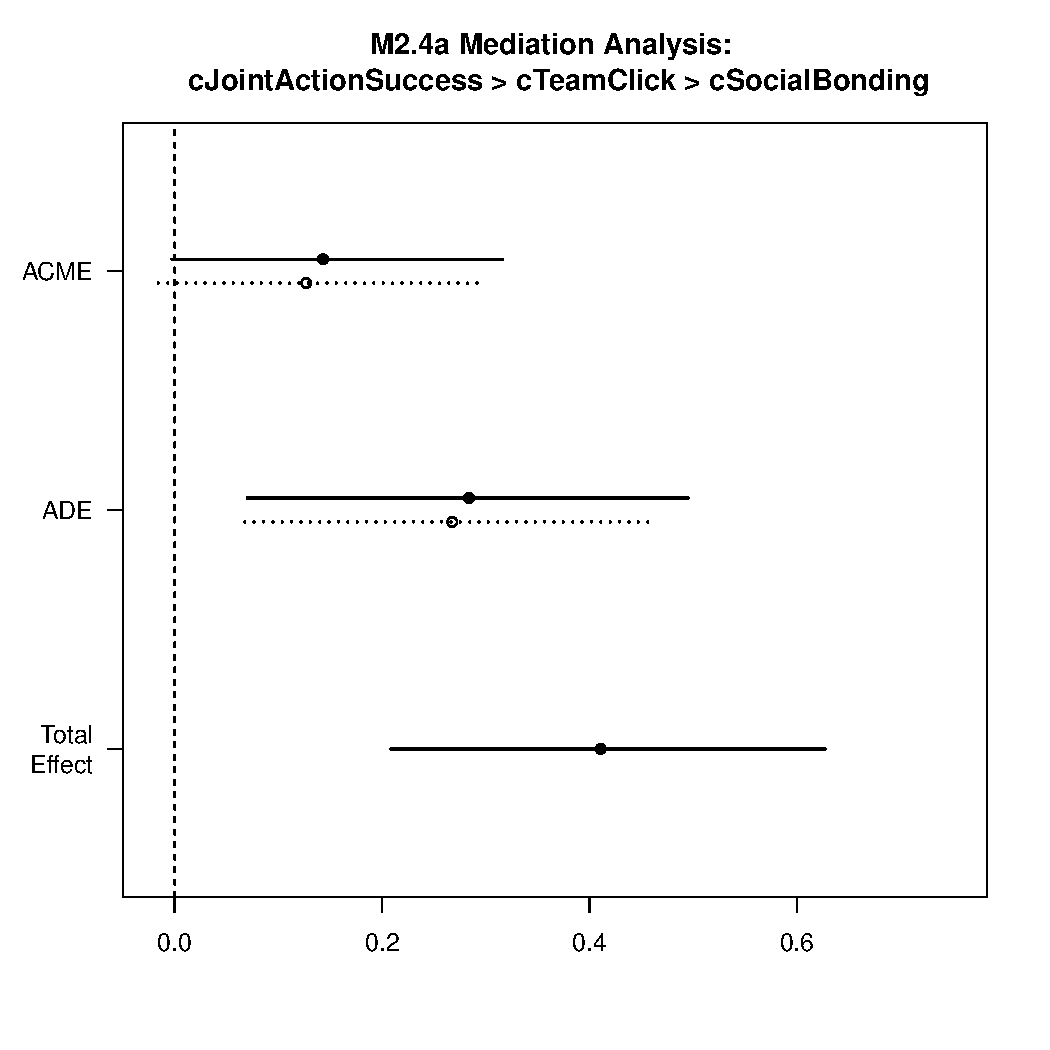
\includegraphics[width=\columnwidth]{images/MLM24aMediationAnalysis.pdf}
  \caption{M24a Mediation Analysis}
  \label{fig:MLM24aMediationAnalysis}
\end{figure}



\subsubsection{Additional Analysis: What predicts change in fusion to family?}
Both verbal and pictorial measures of fusion to team did not vary significantly in pre-post Tournament measures (see descriptives Table ~\ref{tab:factorsPrePostSummary}).  Interestingly, the pictorial measure of fusion to family did increase significantly between pre- and post-Tournament measurements.  Exploratory analysis was performed to investigate the possible correlates of this increase. In line with the predictions of this study, we tested whether 1) changes in perceptions of Joint Action Success, 2) Team Click, and 3) their interaction (Joint Action Success x Team Click) predicted change in fusion to family.

\myparagraph{$\Delta$Fusion Family $\sim$ $\Delta$Joint Action Success}
The first model revealed a significant effect of change in perceptions of joint-action success and change in fusion to family, $\beta = .43$ ($95\% CI =  .07, .79$), $SE = .18$, $t(6.96) = 2.34$, $p = .$, $marginal R^2 = .11$, $conditional R^2 = .14$.  The distribution of residuals indicated a poor model fit, ($W = 0.90$, $p < .00001$), due to high kurtosis ($> 2$), but not skew (.30). Given that log-transformation was not appropriate for normalising kurtosis \citep{Glass1972}, the analysis was re-run after excluding influential outliers.  The adjusted model was a much better fit, with model residuals normally distributed around zero, ($W = 0.99$, $p-value < .60$), see Table ~\ref{tab:MLM25acFusioncJointAction}. The model confirmed a significant positive relationship between change in perceptions of joint-action success and change in fusion to family, $\beta = .36$ ($95\% CI =  .19, .52$), $SE = .08$, $t() = 4.36$, $p = .$, $marginal R^2 = .32$, $conditional R^2 = .32$.


% Table created by stargazer v.5.2 by Marek Hlavac, Harvard University. E-mail: hlavac at fas.harvard.edu
% Date and time: Tue, Jun 27, 2017 - 10:42:15
\begin{table}[!htbp] \centering 
  \caption{cFusionFamily ~ jointActionSuccess} 
  \label{tab:MLM25acFusioncJointAction} 
\footnotesize 
\begin{tabular}{@{\extracolsep{5pt}}lcc} 
\\[-1.8ex]\hline 
\hline \\[-1.8ex] 
 & \multicolumn{2}{c}{\textit{Dependent variable:}} \\ 
\cline{2-3} 
\\[-1.8ex] & cFusionFamily & fusionPictorialFamilyChangeOut \\ 
 &  & outliers removed \\ 
\\[-1.8ex] & (1) & (2)\\ 
\hline \\[-1.8ex] 
 (constant) & 0.12 & $-$0.04 \\ 
  & (0.66) & (0.32) \\ 
  & & \\ 
 cJointActionSuccess & 0.43$^{**}$ & 0.50$^{***}$ \\ 
  & (0.18) & (0.10) \\ 
  & & \\ 
 cIndPerformanceSuccess & $-$0.46$^{**}$ & $-$0.01 \\ 
  & (0.20) & (0.10) \\ 
  & & \\ 
 teamPerformanceExpectations & $-$0.01 & 0.002 \\ 
  & (0.01) & (0.004) \\ 
  & & \\ 
 indPerformanceExpectations & 0.001 & $-$0.003 \\ 
  & (0.01) & (0.004) \\ 
  & & \\ 
 objectiveCompetence & 0.27 & 0.06 \\ 
  & (0.19) & (0.09) \\ 
  & & \\ 
 subjectiveCompetence & 0.06 & $-$0.0003 \\ 
  & (0.16) & (0.08) \\ 
  & & \\ 
 finalRank & 0.10 & $-$0.02 \\ 
  & (0.08) & (0.04) \\ 
  & & \\ 
 minutesTotal & $-$0.002 & 0.01 \\ 
  & (0.01) & (0.004) \\ 
  & & \\ 
\hline \\[-1.8ex] 
Marginal R-squared & .11 & .32 \\ 
Conditional R-squared & .14 & .32 \\ 
Observations & 97 & 97 \\ 
Log Likelihood & $-$173.00 & $-$104.99 \\ 
Akaike Inf. Crit. & 372.00 & 235.98 \\ 
Bayesian Inf. Crit. & 405.48 & 269.45 \\ 
\hline 
\hline \\[-1.8ex] 
\textit{Note:}  & \multicolumn{2}{r}{$^{*}$p$<$0.1; $^{**}$p$<$0.05; $^{***}$p$<$0.01} \\ 
\end{tabular} 
\end{table} 

% Table created by stargazer v.5.2 by Marek Hlavac, Harvard University. E-mail: hlavac at fas.harvard.edu
% Date and time: Tue, Jun 27, 2017 - 10:42:15
\begin{table}[!htbp] \centering 
  \caption{cFusionFamily ~ jointActionSuccess} 
  \label{tab:MLM25acFusioncJointAction} 
\footnotesize 
\begin{tabular}{@{\extracolsep{5pt}} ccc} 
\\[-1.8ex]\hline 
\hline \\[-1.8ex] 
$0.05$ & $0.01$ & $0.001$ \\ 
\hline \\[-1.8ex] 
\end{tabular} 
\end{table} 


%Need to do a multivariate regression here with family, country, team as outcomes?
\myparagraph{$\Delta$fusionFamily $\sim$ $\Delta$Team Click}

This model revealed that change in feelings of team-click was not a significant predictor of change in fusion to family, $\beta = .07$ ($95\% CI =  -.30, .44$), $SE = .19$, $t() = .38$, $p = .$, $marginal R^2 = .04$, $conditional R^2 = .07$. No other predictors in the model were statistically significant.

\myparagraph{$\Delta$fusionFamily $\sim$  $\Delta$Joint Action Success $\times$ $\Delta$Team Click}

The final model included an interaction between change in perceptions of joint-action success and change in feelings of team click as possible predictor of change in fusion to family.  Results of the model revealed that the interaction between change in perceptions of joint-action success and change in feelings of team-click was a significant positive predictor of change in fusion to family, $\beta = .22$ ($95\% CI =  .02, .41$), $SE = .10$, $t() = 2.22$, $p = .$, $marginal R^2 = .17$, $conditional R^2 = .23$. Model residuals were non-normally distributed, ($W = 0.93$, $p < .00001$).\\

This result is consistent with ethnographic findings, whereby the family unit is elevated above the team and other priorities.  This results will be considered in more depth once ethnographic analysis has also been completed.



\subsection{Discussion of Results: pre- to post-Tournament Analysis}
  The results of the pre-post Tournament analysis, like the post-Tournament analysis reported above, provide support for the predictions of this study.  Increases in positive perceptions of joint-action success correlated with a larger increase in feelings of team click pre-post Tournament: athletes who experienced a positive increase in perceptions of joint-action success also reported a positive increase in feelings of team click.  Likewise, those who experienced more positive violations of team performance expectations (measured following the Tournament) also experienced a higher increase in feelings of team click pre-post Tournament.  The interaction between Joint Action Success and Team Performance Expectations, however, was not significant. Further, increases in perception of joint action success (but not team performance expectations) significantly predicted increases in feelings of social bonding before and after the Tournament.  Mediation analysis revealed that variation in team click partially mediated a direct relationship between joint action success and social bonding, however this result was only a significant trend (p = .06).  Team Performance Expectations failed to satisfactorily predict social bonding, and so was not considered in a mediation analysis.












\subsection{Analysis \& results of overall Tournament data}

In the final section of analysis, evidence for a relationship between joint-action success, team click, and social bonding was assessed across the entire data set. Given that the mid-Tournament survey was truncated to accord with athlete schedules and convenience following games, variables that could be analysed across the entire tournament were limited to those that appeared in the mid-Tournament surveys. Time constraints meant that component performance was not assessed in the mid-Tournament survey, and only appraisals of overall individual and team performance relative to prior expectations were included. The mid-Tournament survey contained three team click items (Unspoken Understanding, General Atmosphere, and Click Pictorial), three social bonding items (Emotional Support, Shared Goal, and Fusion Pictorial), and three fatigue items (Fatigue, Physical Exertion, Mental Exertion). These groups of variables were all subjected to data reduction (EFA) for the purposes of analysis.



\subsubsection{Roadmap of Overall Tournament Analysis}
Analysis of the overall Tournament data proceeded in the same step-wise fashion as analyses above. First, the relationship between Team Performance Expectations and team click Team Click was tested, controlling for Tournament performance, perceptions of individual performance, and competence.

\begin{description}
  \item [Prediction 3.1.b] Team Performance Expectations $\rightarrow$ Team Click
\end{description}

Next, the relationship between Team Click and Social Bonding was tested, followed by a test of the direct relationship between Team Performance Expectations and Social Bonding:

\begin{description}
  \item [Prediction 3.2.a] Team Click $\rightarrow$ Social Bonding
  \item [Prediction 3.2.b] Team Performance Expectations $\rightarrow$ Social Bonding
\end{description}
\bigskip
Finally, a mediation analysis was conducted, in which the interaction effect of Team Performance Expectations and team click on social bonding was tested.
\bigskip
\begin{description}
\item[Prediction 3.4.a] Team Performance Expectations^*Team Click  $\rightarrow$ Social Bonding
\item[Prediction 3.4.b] Mediation Analysis: Team Performance Expectations $\rightarrow$ Team Click $\rightarrow$ Social Bonding
\end{description}
\clearpage




\subsubsection{Overall Tournament Descriptive Analysis}

Tables~\ref{tab:performanceOverallSummary}\nobreakdash--\ref{tab:fatigueOverallSummary} display basic summary statistics (mean and standard deviation) for variables of interest at each recorded time point. Almost all variables of interest under the categories of performance, team click, social bonding and fatigue have means above the mid-point of each scale. In addition, mid-Tournament measurements tend to be lower than pre- or post-Tournament measures for each category. In relation to performance measures, for example, athletes appear on average to be more critical of their own and their team’s performance (relative to prior expectations) when surveyed immediately after games on day 1 and 2 than they were following the Tournament (note, however, that survey items relating to individual and team performance administered pre-Tournament were not posed in relation to athlete expectations, and thus could not be directly compared to subsequent mid- and post-Tournament measures). The same pattern was identifiable in team click variables, with the means for mid-Tournament measures of Unspoken Understanding and General Atmosphere 10-15\% lower than pre- or post-Tournament measures. This is also the case for variables related to social bonding: Emotional Support and Shared Goal in particular showing a steep increase form mid-Tournament measurements to the post-Tournament measurement. The same pattern was identifiable for variables relevant to fatigue (see Table ~\ref{tab:fatigueOverallSummary}).


% Table created by stargazer v.5.2 by Marek Hlavac, Harvard University. E-mail: hlavac at fas.harvard.edu
% Date and time: Mon, Jun 26, 2017 - 09:48:21
\begin{table}[!htbp] \centering 
  \caption{Overall Tournament Performance Summary Statistics} 
  \label{tab:performanceOverallSummary} 
\scriptsize 
\begin{tabular}{@{\extracolsep{5pt}} ccccccccc} 
\\[-1.8ex]\hline 
\hline \\[-1.8ex] 
time & teamPerf & tP.sd & indPerf & iP.sd & teamPerfExp & tPE.sd & indPerfExp & iP.sd.1 \\ 
\hline \\[-1.8ex] 
pre-Tournament & $71.11$ & $21.87$ & $68.92$ & $21.32$ & $$ & $$ & $$ & $$ \\ 
day1 & $$ & $$ & $$ & $$ & $54.43$ & $30.63$ & $39.43$ & $27.25$ \\ 
day2 & $$ & $$ & $$ & $$ & $53.19$ & $32.98$ & $40.92$ & $27.93$ \\ 
post-Tournament & $$ & $$ & $$ & $$ & $64.36$ & $23.61$ & $56.36$ & $23.47$ \\ 
\hline \\[-1.8ex] 
\end{tabular} 
\end{table} 


% Table created by stargazer v.5.2 by Marek Hlavac, Harvard University. E-mail: hlavac at fas.harvard.edu
% Date and time: Mon, Jun 26, 2017 - 09:21:29
\begin{table}[!htbp] \centering 
  \caption{Team Click Overall Tournament Summary Statistics} 
  \label{tab:clickOverallSummary} 
\scriptsize 
\begin{tabular}{@{\extracolsep{5pt}} ccccccc} 
\\[-1.8ex]\hline 
\hline \\[-1.8ex] 
time & unspUnd & uU.sd & genAt & gA.sd & clickPic & cP.sd \\ 
\hline \\[-1.8ex] 
pre-Tournament & $71.58$ & $20.77$ & $75.51$ & $23.27$ & $3.87$ & $1.24$ \\ 
day1 & $55.92$ & $26.88$ & $65.74$ & $31.95$ & $3.46$ & $1.49$ \\ 
day2 & $55.30$ & $29.43$ & $64.32$ & $33.39$ & $3.33$ & $1.70$ \\ 
post-Tournament & $72.72$ & $19.95$ & $78.45$ & $21.34$ & $3.93$ & $1.04$ \\ 
\hline \\[-1.8ex] 
\end{tabular} 
\end{table} 


% Table created by stargazer v.5.2 by Marek Hlavac, Harvard University. E-mail: hlavac at fas.harvard.edu
% Date and time: Mon, Jun 26, 2017 - 09:22:14
\begin{table}[!htbp] \centering 
  \caption{Social Bonding Overall Tournament Summary Statistics} 
  \label{tab:bondingOverallSummary} 
\scriptsize 
\begin{tabular}{@{\extracolsep{5pt}} ccccccc} 
\\[-1.8ex]\hline 
\hline \\[-1.8ex] 
time & emoSup & eS.sd & sharedGoal & sG.sd & fusionPic & fP.sd \\ 
\hline \\[-1.8ex] 
pre-Tournament & $70.12$ & $26.21$ & $77.66$ & $24.28$ & $4.26$ & $1.25$ \\ 
day1 & $67.29$ & $30.56$ & $76.34$ & $30.50$ & $4.06$ & $1.47$ \\ 
day2 & $67.53$ & $32.55$ & $71.42$ & $35.47$ & $3.85$ & $1.69$ \\ 
post-Tournament & $79.67$ & $18.84$ & $86$ & $15.56$ & $4.33$ & $1.19$ \\ 
\hline \\[-1.8ex] 
\end{tabular} 
\end{table} 


% Table created by stargazer v.5.2 by Marek Hlavac, Harvard University. E-mail: hlavac at fas.harvard.edu
% Date and time: Mon, Jun 26, 2017 - 09:23:43
\begin{table}[!htbp] \centering 
  \caption{Fatigue Overall Tournament Summary Statistics} 
  \label{tab:fatigueOverallSummary} 
\scriptsize 
\begin{tabular}{@{\extracolsep{5pt}} ccccccccc} 
\\[-1.8ex]\hline 
\hline \\[-1.8ex] 
time & fat & f.sd & prpe & p.sd & mental & m.sd & inj.mu & inj.sd \\ 
\hline \\[-1.8ex] 
pre-Tournament & $$ & $$ & $$ & $$ & $$ & $$ & $18.73$ & $23.36$ \\ 
day1 & $50.14$ & $28.80$ & $12.45$ & $4.52$ & $4.09$ & $2.83$ & $29.91$ & $33.15$ \\ 
day2 & $53.65$ & $31.03$ & $12.60$ & $5.53$ & $4.13$ & $3.17$ & $37.14$ & $37.66$ \\ 
post-Tournament & $69.27$ & $21.24$ & $14.97$ & $2.66$ & $6.08$ & $2.47$ & $23.86$ & $26.91$ \\ 
\hline \\[-1.8ex] 
\end{tabular} 
\end{table} 


%<<surveyMeasureSummaryTable, fig.cap =''>>=
%#create all columns:
%Items <- c(IndPerformance, GroupPerformance, TeamPerformance, GroupClick, TeamClick, GroupBonding, TeamBonding, Arousal, Exertion)
%Baseline <- c("*","","*","","*","","*","","")
%Pre <- c("*","*","","*","","*","","*","")
%Post <- c("*","*","","*","*","*","*","*","*")

%surveyMeasureSummary <- data.frame(Variable, Baseline, Pre, Post, stringsAsFactors = FALSE)

%summaryTable <- xtable(surveyMeasureSummary)
%align(summaryTable) <- xalign(summaryTable)
%summaryTable
%@



\subsubsection{Data Reduction}

Data reduction was performed in order to consolidate outcome variables and reduce multicolinearity of predictor variables. There were only single items for individual and team performance items, and so EFA was not required. Variables relevant to team click, social bonding, and fatigue and measured at each time point across the entire Tournament  were subjected to an EFA.

For Team Click, Unspoken Understanding, General Atmosphere, and Click Pictorial were subjected to EFA.  Correlations between variables were high, suggesting that imposing one factor was appropriate (all $r's > .62$, $KMO = 0.7$, $\chi^2(3, N = 440) = 723.67$).  The factor ``Team Click Tournament'' explained 70.3\% of the variance (SS Loadings = 2.11).  $Guttman's \lambda =.83$ and Cronbach's $\alpha = .87$ indicated that the data reduction was appropriate.

Three variables related to social bonding (Emotional Support, Shared Goal, and Fusion Pictorial) were subjected to EFA. Correlations between variables were high, suggesting that imposing one factor was appropriate (all $r's > .63$, $KMO = 0.71$, $\chi^2(3, N = 440) =  759.30$, $p < .001$).  The factor imposed for Social Bonding (``Social Bonding Tournament'') explained 71.7\% of the variance ($SS Loadings =  2.15$), and $Guttman's \lambda =.84$ and $Cronbach's \alpha= .88$ indicated that the data reduction was reliable.

Fatigue items consisted of fatigue, physical exertion and mental exertion. Correlations between variables were high, indicating that imposing one factor was appropriate (all $r's > .62$, $KMO = 0.71$, $\chi^2(3, N = 440) =  677.37, p < .001$).  The factor imposed for fatigue, ``Fatigue Tournament,'' explained 69\% of the variance ($SS Loading = 2.07$) and $Guttman's \lambda =.82$ and Cronbach's $\alpha = .87$) indicated that the data reduction was reliable.

All other variables used in the Overall Tournament analysis were single item variables and did not require data reduction.





\subsection{Overall Tournament Results}
In the final section, the entire data set was utilised to analyse a relationship between joint-action, team click, and social bonding. As described in the previous section, items relating to performance, team click, and social bonding that were consistent across the data set were reduced to factors in order to test study predictions. The repeated measures design of this analysis made it possible to statistically account for variation in responses due to repeated sampling of the same individual athlete throughout the Tournament, and due to the fact that each athlete was member of a specific team. The following models used a three-level structure, with responses across the four time points (level 1) nested within individual athletes (level 2), who were nested within individual teams (level 3). Both the slopes and intercepts were allowed to vary for every fixed effect of the model.


\subsubsection{3.1.b Team Click $\sim$ Team Performance Expectations}

 The first model tested the predicted relationship between joint-action and team click:
   \begin{equation}

\end{equation}    \begin{align*}
       Team Click =  & Team Performance Expectations  \\
                 &+ Individual Performance Expectations   \\
                 &+ Objective Competence + Subjective Competence \\
                 &+ TournamentPerformanceMeasures  \\
     \end{align*}
   \end{equation}
   \bigskip

 The model revealed a significant relationship between team performance expectation violation and team click, $\beta = .71$ ($95\% CI =  .0.62, .80$), $SE = .001$, $t(193.20) = 16.29$, $p < .0001$, $marginal R^2 = .63$, $conditional R^2 = .69$.
 The model also indicated that individual performance expectation violation significantly predicted team click, $\beta = .004$ ($95\% CI =  .04, .20$), $SE = .04$, $t(311.7) = 2.81$, $p < .01$, as did Subjective Competence, $\beta = .08$ ($95\% CI =  .002, .15$), $SE = .04$, $t(292) = 2.00$, $p = .02$  (see Table ~\ref{tab:MLM31ateamPerfClickTournament} for full description of results).
 The residuals of the model were normally distributed around zero, ($W = 0.99, p = .11$), and individual cases had low influence on the model (Cook's Distances all < .05) (see Appendix Figure ~\ref{fig:MLM31aTeamPerfExpClick}).
 Results of the model suggest that, when controlling for individual performance, measures of objective and subjective competence, and Tournament performance, athletes whose expectations around team performance were more positively violated also experienced stronger feelings of team click. Overall, it also appears that more positive expectations about individual performance, and higher levels of self-reported technical competence predicted higher levels of team click.



 
\begin{table}
\begin{center}
\begin{tabular}{l c c c }
\toprule
 & Intercept & Main effect & Controls \\
\midrule
(constant)                                                        & $-0.00$  & $-0.06$               & $-0.12$               \\
                                                                  & $(0.04)$ & $(0.03)$              & $(0.21)$              \\
Team Performance Vs Expectations                                  &          & $\mathbf{0.74}^{***}$ & $\mathbf{0.72}^{***}$ \\
                                                                  &          & $(0.03)$              & $(0.05)$              \\
Ind Performance Vs Expectations                                   &          &                       & $\mathbf{0.12}^{**}$  \\
                                                                  &          &                       & $(0.04)$              \\
Objective Competence                                              &          &                       & $0.04$                \\
                                                                  &          &                       & $(0.04)$              \\
Subjective Competence                                             &          &                       & $0.07$                \\
                                                                  &          &                       & $(0.04)$              \\
Final Rank                                                        &          &                       & $-0.00$               \\
                                                                  &          &                       & $(0.02)$              \\
Minutes Total                                                     &          &                       & $-0.00$               \\
                                                                  &          &                       & $(0.00)$              \\
Points Total                                                      &          &                       & $0.00$                \\
                                                                  &          &                       & $(0.00)$              \\
Fatigue                                                           &          &                       & $0.00$                \\
                                                                  &          &                       & $(0.00)$              \\
Extraverted                                                       &          &                       & $0.01$                \\
                                                                  &          &                       & $(0.03)$              \\
\midrule
AIC                                                               & 1552.70  & 842.67                & 602.59                \\
BIC                                                               & 1570.04  & 879.53                & 665.89                \\
Log Likelihood                                                    & -772.35  & -412.33               & -284.30               \\
Num. obs.                                                         & 564      & 444                   & 306                   \\
\bottomrule
\multicolumn{4}{l}{\scriptsize{Coefficients with $p < 0.05$ in \textbf{bold}. Marginal $R^2 = .63$, Conditional $R^2 = .69$}}
\end{tabular}
\caption{Prediction 1: Team Performance Vs Expectations predicts Team Click in the Overall Tournament survey data (n = 90).}
\label{tab:MLM31ateamPerfClickTournament}
\end{center}
\end{table}




\subsubsection{3.2.a Social Bonding $\sim$ Team Click}
 The relationship between team click and social bonding was tested. Controlling for perceptions of individual performance, measures of objective and subjective competence, and Tournament performance, the model revealed a significant positive relationship between feelings of team click and feelings of social bonding, $\beta = .64$ ($95\% CI = .56, .74$), $SE = .05$, $t(87.4) = 13.84$, $p < .0001$, $marginal R^2 = .49$, $conditional R^2 = .66$ (see Table ~\ref{tab:MLM31bclickBondingTournament} for complete description of model estimates). Model residuals were not normally distributed around zero, ($W = 0.92, p < .00001$), owing to high negative skew ($-1.24$) and high kurtosis (5.12) (see Appendix Figure ~\ref{fig:MLM31bAssumptions}).
 Both log transformation ($W = 0.95, p < .00001$) and outlier removal ($W = 0.96, p < .00001$) procedures improved the model fit marginally, but not within the bounds of normality.
 To resolve this assumption violation, the outcome variable was first subjected to outlier-removal, and then subsequently log-transformed, which appeared to improve the distribution of residuals somewhat, ($W = 0.98, p = .0002$, see Table ~\ref{MLM31bclickBondingTournamentModelComparison} for adjusted model comparisons and Appendix Figure ~\ref{fig:MLM31bLogOutAssumptions} for adjusted model residuals).
 The adjusted model failed to converge, and so a

 confirmed a significant positive effect of team click on social bonding over the course of the Tournament, $\beta = .19$ ($95\% CI =  .15, .23$), $SE = .05$, $t() = 9.89$, $p < .001$, $marginal R^2 = .30$, $conditional R^2 = .43$.  These results suggest that on average, athletes who experienced higher feelings of team click also experienced higher levels of social bonding throughout the course of the Tournament.

 
% Table created by stargazer v.5.2 by Marek Hlavac, Harvard University. E-mail: hlavac at fas.harvard.edu
% Date and time: Thu, Sep 14, 2017 - 09:39:55
\begin{table}[!htbp] \centering 
  \caption{bondingTournament ~ teamClickTournament} 
  \label{tab:MLM31bclickBondingTournament} 
\footnotesize 
\begin{tabular}{@{\extracolsep{5pt}}lccc} 
\\[-1.8ex]\hline 
\hline \\[-1.8ex] 
 & \multicolumn{3}{c}{\textit{Dependent variable:}} \\ 
\cline{2-4} 
\\[-1.8ex] & (1) & (2) & (3)\\ 
\hline \\[-1.8ex] 
 (constant) & $-$0.00 & $-$1.46$^{***}$ & $-$1.59$^{***}$ \\ 
  & (0.04) & (0.08) & (0.15) \\ 
  & & & \\ 
 teamPerformanceExpectations &  & 0.02$^{***}$ & 0.02$^{***}$ \\ 
  &  & (0.001) & (0.001) \\ 
  & & & \\ 
 indPerformanceExpectations &  &  & 0.004$^{**}$ \\ 
  &  &  & (0.002) \\ 
  & & & \\ 
 objectiveCompetence &  &  & 0.02 \\ 
  &  &  & (0.04) \\ 
  & & & \\ 
 subjectiveCompetence &  &  & 0.08$^{*}$ \\ 
  &  &  & (0.04) \\ 
  & & & \\ 
 finalRank &  &  & $-$0.0002 \\ 
  &  &  & (0.02) \\ 
  & & & \\ 
 minutesTotal &  &  & $-$0.001 \\ 
  &  &  & (0.002) \\ 
  & & & \\ 
 pointsTotal &  &  & 0.003 \\ 
  &  &  & (0.003) \\ 
  & & & \\ 
\hline \\[-1.8ex] 
Marginal R-squared & .47 & .49 &  \\ 
Conditional R-squared & .66 & .66 &  \\ 
Observations & 564 & 444 & 331 \\ 
Log Likelihood & $-$772.35 & $-$412.33 & $-$303.82 \\ 
Akaike Inf. Crit. & 1,552.70 & 842.67 & 637.65 \\ 
Bayesian Inf. Crit. & 1,570.04 & 879.53 & 694.68 \\ 
\hline 
\hline \\[-1.8ex] 
\textit{Note:}  & \multicolumn{3}{r}{$^{*}$p$<$0.05; $^{**}$p$<$0.01; $^{***}$p$<$0.001} \\ 
\end{tabular} 
\end{table} 


 
% Table created by stargazer v.5.2 by Marek Hlavac, Harvard University. E-mail: hlavac at fas.harvard.edu
% Date and time: Thu, Sep 14, 2017 - 09:39:58
\begin{table}[!htbp] \centering 
  \caption{Model Adjustment Comparison:bondingTournament ~ teamClickTournament} 
  \label{MLM31bclickBondingTournamentModelComparison} 
\tiny 
\begin{tabular}{@{\extracolsep{5pt}}lcccc} 
\\[-1.8ex]\hline 
\hline \\[-1.8ex] 
 & \multicolumn{4}{c}{\textit{Dependent variable:}} \\ 
\cline{2-5} 
 & model & log-transformed & outliers removed & outliers + log-transformed \\ 
\\[-1.8ex] & (1) & (2) & (3) & (4)\\ 
\hline \\[-1.8ex] 
 (constant) & $-$1.59$^{***}$ & 1.63$^{***}$ & 0.31$^{***}$ & 1.50$^{***}$ \\ 
  & (0.15) & (0.02) & (0.08) & (0.04) \\ 
  & & & & \\ 
 teamPerformanceExpectations & 0.02$^{***}$ &  &  &  \\ 
  & (0.001) &  &  &  \\ 
  & & & & \\ 
 indPerformanceExpectations & 0.004$^{**}$ &  &  &  \\ 
  & (0.002) &  &  &  \\ 
  & & & & \\ 
 objectiveCompetence &  & 0.16$^{***}$ & 0.42$^{***}$ & 0.19$^{***}$ \\ 
  &  & (0.01) & (0.04) & (0.02) \\ 
  & & & & \\ 
 subjectiveCompetence & 0.02 & 0.01 & 0.01 & 0.01 \\ 
  & (0.04) & (0.01) & (0.03) & (0.01) \\ 
  & & & & \\ 
 finalRank & 0.08$^{*}$ & 0.01 & 0.03 & 0.02 \\ 
  & (0.04) & (0.01) & (0.02) & (0.01) \\ 
  & & & & \\ 
 minutesTotal & $-$0.0002 & $-$0.004 & $-$0.01 & $-$0.01 \\ 
  & (0.02) & (0.003) & (0.01) & (0.005) \\ 
  & & & & \\ 
 pointsTotal & $-$0.001 & $-$0.001 & $-$0.002 & $-$0.001 \\ 
  & (0.002) & (0.0004) & (0.001) & (0.001) \\ 
  & & & & \\ 
 pointsTotal & 0.003 & $-$0.001 & $-$0.001 & $-$0.001 \\ 
  & (0.003) & (0.001) & (0.002) & (0.001) \\ 
  & & & & \\ 
\hline \\[-1.8ex] 
Marginal R-squared & .49 & .50 & .23 & .23 \\ 
Conditional R-squared & .66 & .61 & .35 & .34 \\ 
Shapiro-Wilk Test (p-value) & .92(<.00000000001) & .95(<.000001) & .96(<.00001) & .98(.0002) \\ 
Observations & 331 & 449 & 405 & 405 \\ 
Log Likelihood & $-$303.82 & 225.59 & $-$241.97 & 79.71 \\ 
Akaike Inf. Crit. & 637.65 & $-$423.18 & 511.94 & $-$131.42 \\ 
Bayesian Inf. Crit. & 694.68 & $-$365.69 & 567.99 & $-$75.37 \\ 
\hline 
\hline \\[-1.8ex] 
\textit{Note:}  & \multicolumn{4}{r}{$^{*}$p$<$0.05; $^{**}$p$<$0.01; $^{***}$p$<$0.001} \\ 
\end{tabular} 
\end{table} 



\subsubsection{3.2.b Social Bonding $\sim$ Team Performance Expectations}
The direct relationship between Team Performance Expectations and social bonding was tested.  The initial model failed to converge with the random slope and intercept model structure.  As such, the model was simplified to estimate only the random slope. This simplified model revealed a significant positive relationship between team performance expectation violation and social bonding, $\beta = .46$ ($95\% CI =  .35, .57$), $SE = .05$, $t(331.00) = 8.48$, $p < .0001$, $marginal R^2 = .40$, $conditional R^2 = .40$.
The model also revealed a significant relationship between Individual Performance Expectations and social bonding, $\beta = .005$ ($95\% CI =  .002, .009$), $SE = .002$, $t(303.4) = 2.80$, $p < .01$, as well as subjective competence and social bonding, $\beta = .01$ ($95\% CI =  .01, .18$), $SE = .04$, $t(265.3) = 2.24$, $p = .03$ (see Table ~\ref{tab:MLM32ateamPerfBondingTournament} for full description of model estimates).

Model residuals were non-normally distributed, ($W = 0.97, p < .00001$), with negative skew ($-.6$), and higher than normal kurtosis, see Appendix Figure ~\ref{fig:MLM32aAssumptions}.  A model in which the outcome was log-transformed following removal of outliers provided the best possible fit for the available data ~\ref{MLM32ateamPerfBondingTournamentModelComparison}. While the distribution of errors was still non-normal, ($W = 0.99, p = .03$),  error terms appear much more evenly distributed around zero than the original model, albeit with a slight negative skew ($-0.1$).
The adjusted model confirmed the significant positive effect of team performance expectation violation on social bonding,  $\beta = .16$ ($95\% CI =  .12, .20$), $SE = .02$, $t(336.80) = 7.98$, $p < .0001$, $marginal R^2 = .36$, $conditional R^2 = .36$.



 
\begin{table}
\begin{center}
\begin{tabular}{l c c c c }
\toprule
 & Main effect & Controls & Log-transformed & Log and outliers \\
\midrule
(constant)                        & $-0.00$               & $\mathbf{0.51}^{*}$   & $\mathbf{1.71}^{***}$ & $\mathbf{1.64}^{***}$ \\
                                  & $(0.04)$              & $(0.26)$              & $(0.06)$              & $(0.08)$              \\
Team Performance Vs Expectations  & $\mathbf{0.59}^{***}$ & $\mathbf{0.47}^{***}$ & $\mathbf{0.11}^{***}$ & $\mathbf{0.07}^{***}$ \\
                                  & $(0.04)$              & $(0.06)$              & $(0.01)$              & $(0.02)$              \\
Ind Performance Vs Expectations   &                       & $\mathbf{0.25}^{***}$ & $\mathbf{0.05}^{***}$ & $0.01$                \\
                                  &                       & $(0.06)$              & $(0.01)$              & $(0.02)$              \\
Objective Competence              &                       & $0.07$                & $0.02$                & $0.01$                \\
                                  &                       & $(0.05)$              & $(0.01)$              & $(0.02)$              \\
Subjective Competence             &                       & $0.09$                & $\mathbf{0.02}^{*}$   & $\mathbf{0.03}^{*}$   \\
                                  &                       & $(0.05)$              & $(0.01)$              & $(0.01)$              \\
Final Rank                        &                       & $-0.03$               & $-0.01$               & $-0.01$               \\
                                  &                       & $(0.02)$              & $(0.01)$              & $(0.01)$              \\
Minutes Total                   &                       & $-0.01$  & $-0.00$  & $-0.00$               \\
                                  &                       & $(0.00)$              & $(0.00)$              & $(0.00)$              \\
Points Total                      &                       & $0.00$                & $0.00$                & $0.00$                \\
                                  &                       & $(0.00)$              & $(0.00)$              & $(0.00)$              \\
Fatigue                           &                       & $0.00$                & $0.00$                & $0.00$                \\
                                  &                       & $(0.00)$              & $(0.00)$              & $(0.00)$              \\
Extraverted                       &                       & $-0.04$               & $-0.01$               & $-0.02$               \\
                                  &                       & $(0.03)$              & $(0.01)$              & $(0.01)$              \\
\midrule
AIC                               & 1083.79               & 752.42                & -131.94               & -8.28                 \\
BIC                               & 1104.27               & 800.83                & -83.53                & 38.54                 \\
Log Likelihood                    & -536.89               & -363.21               & 78.97                 & 17.14                 \\
Num. obs.                         & 444                   & 306                   & 306                   & 271                   \\
\bottomrule
\multicolumn{5}{l}{\scriptsize{Coefficients with $p < 0.05$ in \textbf{bold}. Effect sizes of the Log and outlier model: Marginal $R^2 = .36$, Conditional $R^2 = .36$}}
\end{tabular}
\caption{Prediction 3: Team Performance Vs Expectations predicts Social Bonding in the Overall Tournament survey data (n = 90).}
\label{tab:MLM32ateamPerfBondingTournament}
\end{center}
\end{table}


 
% Table created by stargazer v.5.2 by Marek Hlavac, Harvard University. E-mail: hlavac at fas.harvard.edu
% Date and time: Thu, Sep 14, 2017 - 09:42:11
\begin{table}[!htbp] \centering 
  \caption{Model Comparison: M3.2a socialBondingTournament ~ teamPerformanceExpectationsTournament} 
  \label{tab:MLM32ateamPerfBondingTournamentModelComparison} 
\scriptsize 
\begin{tabular}{@{\extracolsep{5pt}}lccc} 
\\[-1.8ex]\hline 
\hline \\[-1.8ex] 
 & \multicolumn{3}{c}{\textit{Dependent variable:}} \\ 
\cline{2-4} 
 & model & log-transformed & outliers+log-transformed \\ 
\\[-1.8ex] & (1) & (2) & (3)\\ 
\hline \\[-1.8ex] 
 (constant) & $-$0.70$^{***}$ & 1.42$^{***}$ & 1.42$^{***}$ \\ 
  & (0.18) & (0.04) & (0.06) \\ 
  & & & \\ 
 teamPerformanceExpectations & 0.01$^{***}$ & 0.003$^{***}$ & 0.003$^{***}$ \\ 
  & (0.002) & (0.0005) & (0.001) \\ 
  & & & \\ 
 indPerformanceExpectations & 0.01$^{**}$ & 0.001$^{**}$ & 0.0001 \\ 
  & (0.002) & (0.0004) & (0.001) \\ 
  & & & \\ 
 objectiveCompetence & 0.04 & 0.01 & 0.01 \\ 
  & (0.05) & (0.01) & (0.02) \\ 
  & & & \\ 
 subjectiveCompetence & 0.10$^{*}$ & 0.03$^{*}$ & 0.03$^{*}$ \\ 
  & (0.04) & (0.01) & (0.01) \\ 
  & & & \\ 
 finalRank & $-$0.04 & $-$0.01 & $-$0.01 \\ 
  & (0.02) & (0.005) & (0.01) \\ 
  & & & \\ 
 minutesTotal & $-$0.003 & $-$0.001 & $-$0.001 \\ 
  & (0.002) & (0.001) & (0.001) \\ 
  & & & \\ 
 pointsTotal & 0.001 & 0.0001 & 0.0000 \\ 
  & (0.004) & (0.001) & (0.001) \\ 
  & & & \\ 
\hline \\[-1.8ex] 
Marginal R-squared & .33 & .11 & .09 \\ 
Conditional R-squared & .53 & .23 & .17 \\ 
Shapiro-Wilk Test (p-value) & .97($<$.00001) & .96($<$.00001) & .97($<$.00001) \\ 
Observations & 331 & 331 & 294 \\ 
Log Likelihood & $-$373.85 & 96.45 & 21.56 \\ 
Akaike Inf. Crit. & 777.70 & $-$162.91 & $-$13.13 \\ 
Bayesian Inf. Crit. & 834.73 & $-$105.88 & 42.13 \\ 
\hline 
\hline \\[-1.8ex] 
\textit{Note:}  & \multicolumn{3}{r}{$^{*}$p$<$0.05; $^{**}$p$<$0.01; $^{***}$p$<$0.001} \\ 
\end{tabular} 
\end{table} 





\subsubsection{3.4.a Social Bonding $\sim$ Team Performance Expectations Tournament $\times$ Team Click Tournament}

 The interaction of Team Performance Expectations and Team Click was added to the model as a fixed effect to see if an increase in social bonding associated with more positive violations of team performance expectations was heightened when feelings of team-click increased. The model revealed a significant negative interaction between Team Performance Expectations and Team Click,  $\beta = -.26$ ($95\% CI =  -.32, -.20$), $SE = .03$, $t(321.2) = -8.46$, $p < .0001$, $marginal R^2 = .69$, $conditional R^2 = .74$.  Model residuals were non-normal ($W = 0.94, p < .00001$), owing to high kurtosis ($.39$) and negative skew ($-.88$) (see Appendix Figure ~\ref{fig:MLM32aAssumptions}).
 A model in which the outcome variable was log transformed following exclusion of outliers provided the best adjustment: model residuals were normally distributed ($W = 0.99, p = .14$) and individual observations exerted low influence (Cook's Distances all < .10) (see Table ~\ref{MLM33ateamPerfBondingTournamentInteractionComparison} for full model comparison). The adjusted model revealed a significant positive interaction of Team Performance Expectations and Team Click on Social Bonding, $\beta = -.06$ ($95\% CI =  .0004, .002$), $SE = .01$, $t(310.1) = -4.73$, $p < .001$, $marginal R^2 = .61$, $conditional R^2 = .65$.

 These results supported the prediction that feelings of team-click condition the relationship between perceptions of team performance (expectation violation, in this case) and feelings of social bonding.  Below, formal mediation analysis was conducted to further test this relationship.


 
% Table created by stargazer v.5.2 by Marek Hlavac, Harvard University. E-mail: hlavac at fas.harvard.edu
% Date and time: Thu, Sep 14, 2017 - 09:52:55
\begin{table}[!htbp] \centering 
  \caption{M3.3a socialBondingTournament ~ teamPerformanceExpectationsTournament*teamClickTournament} 
  \label{tab:MLM33ateamPerfBondingTournamentInteractionComparison} 
\scriptsize 
\begin{tabular}{@{\extracolsep{5pt}}lccc} 
\\[-1.8ex]\hline 
\hline \\[-1.8ex] 
 & \multicolumn{3}{c}{\textit{Dependent variable:}} \\ 
\cline{2-4} 
 & model & log-transformed & outliers+log-transformed \\ 
\\[-1.8ex] & (1) & (2) & (3)\\ 
\hline \\[-1.8ex] 
 (constant) & 0.45$^{**}$ & 1.69$^{***}$ & 1.62$^{***}$ \\ 
  & (0.16) & (0.04) & (0.06) \\ 
  & & & \\ 
 teamPerformanceExpectations & $-$0.0001 & $-$0.0003 & $-$0.001 \\ 
  & (0.002) & (0.0004) & (0.001) \\ 
  & & & \\ 
 indPerformanceExpectations & 1.02$^{***}$ & 0.22$^{***}$ & 0.11$^{**}$ \\ 
  & (0.06) & (0.01) & (0.04) \\ 
  & & & \\ 
 objectiveCompetence & 0.001 & 0.0003 & $-$0.0001 \\ 
  & (0.001) & (0.0004) & (0.001) \\ 
  & & & \\ 
 subjectiveCompetence & 0.01 & 0.01 & 0.01 \\ 
  & (0.04) & (0.01) & (0.01) \\ 
  & & & \\ 
 finalRank & 0.05 & 0.01 & 0.02 \\ 
  & (0.04) & (0.01) & (0.01) \\ 
  & & & \\ 
 minutesTotal & $-$0.03$^{*}$ & $-$0.01$^{*}$ & $-$0.01 \\ 
  & (0.02) & (0.004) & (0.01) \\ 
  & & & \\ 
 pointsTotal & $-$0.003 & $-$0.001 & $-$0.001 \\ 
  & (0.002) & (0.0005) & (0.001) \\ 
  & & & \\ 
 pointsTotal & 0.001 & 0.0001 & $-$0.001 \\ 
  & (0.003) & (0.001) & (0.001) \\ 
  & & & \\ 
 teamPerformanceExpectations:clickFactor3 & $-$0.01$^{***}$ & $-$0.002$^{***}$ & 0.002$^{*}$ \\ 
  & (0.001) & (0.0003) & (0.001) \\ 
  & & & \\ 
\hline \\[-1.8ex] 
Marginal R-squared & .68 & .28 & .23 \\ 
Conditional R-squared & .73 & .36 & .28 \\ 
Shapiro-Wilk Test (p-value) & .93($<$.00001) & .99(.02) & .99(.14) \\ 
Observations & 331 & 331 & 294 \\ 
Log Likelihood & $-$277.92 & 176.98 & 57.06 \\ 
Akaike Inf. Crit. & 589.83 & $-$319.96 & $-$80.12 \\ 
Bayesian Inf. Crit. & 654.47 & $-$255.32 & $-$17.50 \\ 
\hline 
\hline \\[-1.8ex] 
\textit{Note:}  & \multicolumn{3}{r}{$^{*}$p$<$0.05; $^{**}$p$<$0.01; $^{***}$p$<$0.001} \\ 
\end{tabular} 
\end{table} 








%  plot() interaction





\subsubsection{3.4.b Mediation Analysis: Team Performance Expectations -> Team Click -> Social Bonding}

A mediation analysis was performed to formally test whether feelings of team click over the course of the Tournament mediated a direct relationship between team performance expectation violations and social bonding.  Results outlined above demonstrate Tournament-wide significant positive relationships between team performance expectation violations and feelings of team click, as well as team click and social bonding. Models also demonstrate a direct relationship between expectations around team performance and social bonding.  Available statistical software can only support a 2-level structure for multilevel mediation analysis. The third team-level random effect was therefore dropped from the model, while the model controlled for the random effect of individual across each of the four time points.

Results of the mediation analysis revealed that the average indirect effect of change in Joint Action Success on change in Social Bonding attributable to change in Team Click was highly significant albeit small, $\beta = .02, 95\% CI = .018 , .026, p < .001$.  When controlling for the effect of team click on social bonding, the average direct effect of Team Performance Expectations and Social Bonding was also significant, $\beta = .01, 95\% CI = .001 , .017, p < .00001$.  The total effect of the meditation was also significant, $\beta = .03, 95\% CI = .027, .041, p < .0001$ (see Appendix Figure ~\ref{fig:MLM34aMediationAnalysis}).
These results suggest that Team Click \textit{partially} mediates the effect of Team Performance Expectations and Social Bonding (average proportion mediated = .66 (.57, .77)).  This result should be treated with additional caution, as it did not account for team-level variation.


\begin{figure}[htbp]
  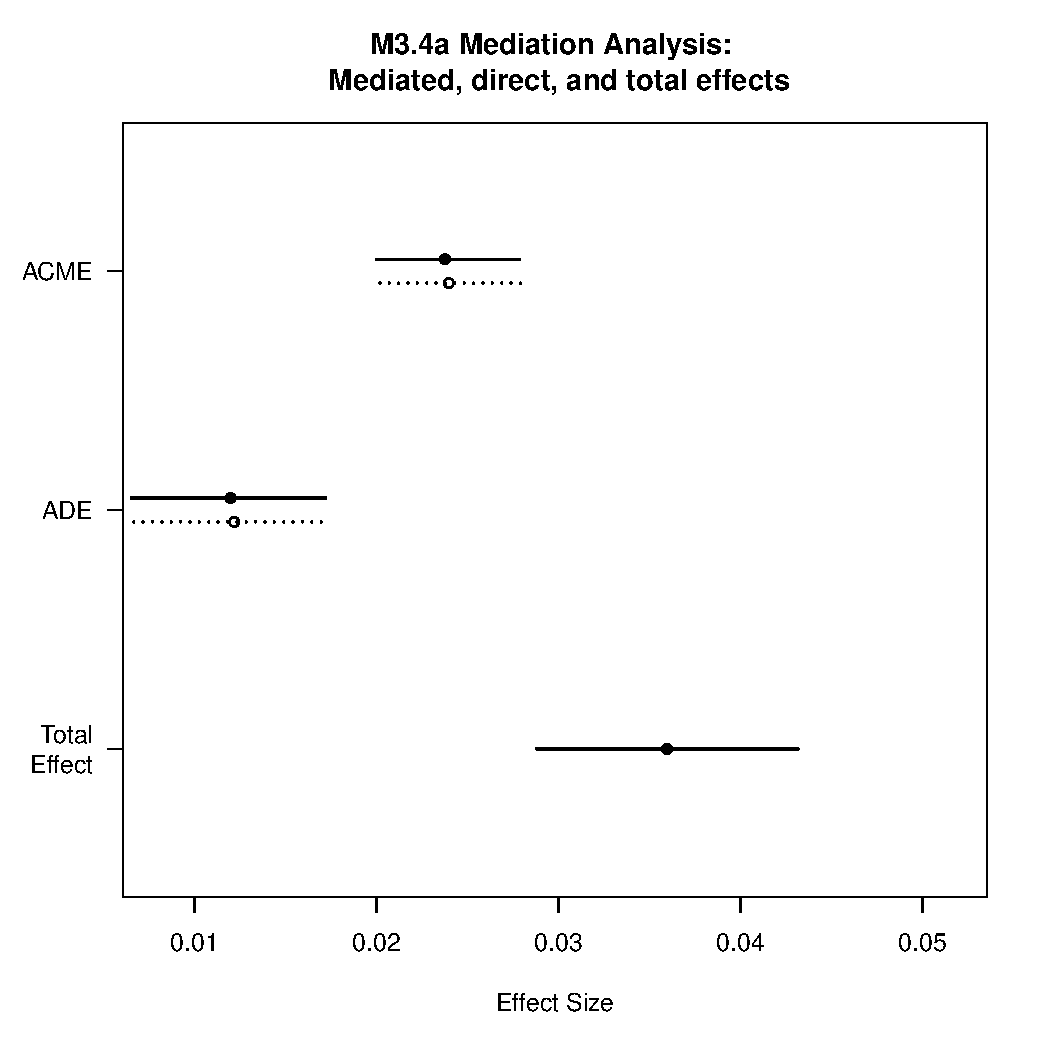
\includegraphics[width =\columnwidth]{images/MLM34aMediationAnalysis.pdf}
  \caption{M3.4a Mediation Analysis}
  \label{fig:MLM34aMediationAnalysis}
\end{figure}


\subsubsection{Discussion of overall Tournament results}





  \section{Discussion of Results}

  The results presented above generally support the central hypothesis of this dissertation, namely that relationship the relationship between joint action and social bonding is mediated by the feeling of ``team click.''  Results of analyses concerning both the post-Tournament survey and change between and pre- and post -Tournament surveys display a clear relationship between perceptions of Joint Action Success and Team Click, Team Click and Social Bonding, and a direct relationship between Joint Action Success and Social Bonding.  In the post-Tournament analysis, Team Click fully mediates the relationship between Joint Action Success and Social Bonding. In the pre-post analysis, Team Click partially mediates this relationship (this statistic was not significant, but was trending in the predicted direction, $p = .06$).

  Results of models designed to test the predicted relationships between Team Performance Expectations, Team Click, and Social Bonding also provided support for some but not all predictions. A relationship was confirmed between team performance expectation violation and team click, but not between expectation violation and social bonding. In addition, the predicted interaction between Joint Action Success, Team Performance Expectations, and Team Click was not significant, nor was the interaction between these same two predictor variables and social bonding.  Team click did not mediate the predicted relationship between violations of expectations around team performance and social bonding. The model of this direct relationship was not statistically robust using the data collected in this study.

  These results suggests that while expectation violation in joint action might be an important factor in generating feelings of team click, it might not be a strong enough mechanism to drive social bonding directly.  In contrast to the single-item measure of Team Performance Expectations, Joint Action Success is a factor made up of four items that require detailed reflection on the experience of four different aspects of team coordination.  This item may have more powerfully tapped into the implicit mechanisms involved in coordinated joint action, encouraging athletes to reflect on coordination with specific co-actors, and as such the opportunity to rehearse and reinforce feelings of trust, reliability, and cooperation \citep{Reddish2013a}.  It is also possible that expectation violation in joint action might not be immediately available to athlete reflection.
  As Frith and colleagues point out \textcite{Frith2007,Frith2010,Clark2013}, the generation of interoceptive predictive models for action implicates cognitive processes that exist largely below the surface of conscious awareness, and the relationship between these unconscious informational transfer in movement coordination and the small fraction of information that does make its way to consciousness in the form of higher order symbolic and linguistic representations is still not clearly understood \citep{Semin2008}. Team click might be supported by various subtle, implicit, and pre-perceptual processes involved in ``active inference'' \citep{Schmidt2011}.

  Evidence presented here does however support the interpretations that perceptions of joint action success predict social bonding, mediated by the experience of ``team click.'' It was predicted that technical competence may condition the relationship between perceptions of joint action, team click, and social bonding, owing to the possibility that more expert athletes could be more likely experience less pronounced discrepancy between expected and actual performance \cite{Tomeo2012}.  In this specific study, there was no evidence that technical competence---objective competence (training age, years in team, age) and self-reported competence (ability versus teammates, Chinese opponents, or international professionals)---significantly influenced variables of interest.  It is possible, as noted above, that these measures failed to access the (largely pre-perceptual) mechanisms of prediction error management hypothesised to underpin cognition and affective dispositions in joint action.  It is also possible that the nature of the intensity and consequentiality of the Tournament in which athletes were participating was high enough that no one---experts athletes included---was immune to the uncertainty and stress of this experience. Indeed, the ability of competitive group exercise contests to consistently arouse high levels of psychological stress and uncertainty could be an important reason for their cultural evolutionary success over recent centuries.

  In addition to technical competence of individual athletes, preexisting dispositional tendencies in dimensions of personality (e.g., extroversion, agreeableness) and physical endowment could impact on processes of social bonding \citep{Marsh2009,VonRueden2015}.   It has been documented that personality types correspond with basal tendencies for movement and movement coordination. In a joint action task involving two people of different heights moving wooden planks of different lengths, for example, Richardson and colleagues \textcite{Richardson2007} found that individuals’ levels of agreeableness and extroversion were positively correlated with the level of persistence of cooperation (hyteresis).  In particular, in the condition in which wooden planks increased in length (therefore increasing in demand for cooperative action), the degree of cooperation was positively correlated with the taller of the pair’s extroversion; the degree of cooperation in the random condition (where planks were received in no ordinal sequence of sizing) was correlated with the agreeableness of the shorter (i.e., more constraining) of the individuals.  I used the personality data collected in the pre-Tournament survey to test the relationship between personality types and team click. Interestingly, none of the big five personality types (extraversion, agreeableness, openness, conscientiousness, and neuroticism) significantly predicted feelings of team click in the post-Tournament survey.

  The impact of inter-individual psychophysiological variation on joint action can also be seen in the case of social dysfunctions such as autism spectrum disorder \citep{Isenhower2012} and schizophrenia \citep{Varlet2012}.  Generally speaking,  while autism spectrum disorder appears to be associated with deficits in anticipatory timing adjustments in intra- and inter-individual coordination of physical movement \citep{Martineau2010}, schizophrenia appears linked to a lack of prediction error management, due to failure in the neurological mechanisms through which predictions about the consequences of an action are derived \citep{Frith2000}.  Delusions of control owing to misattribution of agency are well-documented in schizophrenic patients---either delusions of self-control over external actions and events, or, alternatively, delusions involving the control of others over the individual (in the case of split personality and associated hallucinations) \citep{Frith2007}. It is quite possible that the experience of ``team click'' is an analogue, albeit much socially functional, to the pathological over-activity of agency-attribution mechanisms observed in schizophrenic patients.  The question of individual variation in sociability and movement tendencies should be further assessed in future studies.

  The fact that the hypothesised mechanisms of joint action and social bonding have been shown to exist pre-declaratively and predominantly below the surface of conscious experience presents a methodological challenge for psychological research which relies heavily on self-report.  Further exploring the relationship between pre-perceptual regulatory mechanisms of joint action and their psychosocial effects will require the use of other methods of data collection and analysis in order to triangulate the reliability of self-report data \citep{Newell2014}.  In this specific example, video footage showing athlete performance and coordination could be assessed using already established methods of motion capture and analysis to provide pseudo-objective measures of interpersonal and team-level synchrony in joint action \citep[e.g.][]{Passos2011}.
  Importantly, video footage analysis allows for the testing between different proposed mechanisms associated with joint action and social bonding,  For example, motion capture from video footage allows for measuring synchrony between co-actors could using both traditional methods of dimension reduction and principal component analysis \citep[see for example][]{Riley2011} as well as emerging methods borrowed from dynamic systems theory including fractal-like 1/f scaling (``pink noise'') \citep[see for example][]{Holden2013}. It is quite possible that these different measurements of synchrony could access different psychophysiological dimensions of the relationship between joint action and social bonding.  Other physiological markers of social interaction such as heart rate variability \citep{Konvalinka2011,Fischer2014a} and pain threshold \citep{Cohen2009,Tarr2015}) are beginning to be developed and tested in both experimental and real-world settings.
  These novel methodological approaches help complement existing behavioural measures, such as such as economic games \citep{Xygalatas2013} and spontaneous helping tasks \citep{Kirschner2010}, designed to access psychological mechanisms related to social bonding and cooperation.
  Together, these measures could then be compared to self-report measures derived from athlete self-report to more fully understand the ways in which component mechanisms and system dynamics of joint action generate social cohesion \citep{Marsh2009}.

  In sum, the results reported in this study provide novel evidence that feelings of team click mediate a relationship between perceived joint action success and social bonding, substantiating the claim that under certain circumstances joint action and interpersonal coordination processes can generate feelings of social connection \citep{Marsh2009}. Relationships between expectation violation, team click, and social bonding
  also confirmed, but these models are less robust, and should be treated with caution. All reported results hold when statistically controlling for measures relating to individual performance, objective competence, and actual Tournament performance outcomes in the Tournament, including Tournament rank, points scored, minutes played, and so on.  Of course, the uncontrolled and \textit{in-situ} design of this study means that results are correlational, and as such the predictions of this dissertation, only partially confirmed in this study, require further attention via a controlled experimental design.  An experiment in which joint action success and expectation violation were manipulated, and explicit feedback around performance was eliminated, could allow for the assessment of the role of the cognitive processes of movement coordination in joint action in generating team click and social bonding.  In addition, a controlled experiment offers the opportunity to utilise other measurements of synchrony, such as those derived from motion capture from video recordings.





%    [ ] what inferences can we make from these results?
%    [ ] How does it relate to other literature?
%    [ ] limitations
%    [ ] future work —> experiment (takes away explicit feedback)
%    [ ]  "Conclude the general discussion with a strong paragraph stating the main point or points again, in somewhat different terms-if possible-than used before.”
